\documentclass[12pt,openright]{book}

%%% Packages

% Setting up page
\usepackage[a4paper,top=1in,right=1in,bottom=1in,left=40mm]{geometry}
\usepackage{emptypage}

% Mathematics
\usepackage{amsmath}
\usepackage{amssymb}
\usepackage{amsthm}
\usepackage{mathptmx}
\usepackage{mathtools}

% Fonts and typesetting
\usepackage{./fonts}
\usepackage{datetime}
    \newdateformat{monthyeardate}{\monthname[\THEMONTH] \THEYEAR}
\usepackage{setspace}
    \onehalfspacing%
\usepackage{enumerate}  % Roman numerals in lists

% Page headers and footers
\usepackage{fancyhdr}
\usepackage{etoolbox}

\renewcommand{\chaptermark}[1]{%
    \markboth{\MakeUppercase{\thechapter.\ #1}}{}  % Number and title only
}

\renewcommand{\sectionmark}[1]{%
    \markright{\MakeUppercase{\thesection.\ #1}}{}  % Number and title only
}

\fancypagestyle{normal}{  % Used for most pages
    \fancyhf{}
    \fancyhead[LE]{\slshape\leftmark}  % Show chapter title on left outer leaf
    \fancyhead[RO]{\slshape\rightmark}  % Show section title on right outer leaf
    \fancyfoot[C]{\thepage}  % Show page number on outer leaf
    \renewcommand{\headrulewidth}{1pt}
}

\fancypagestyle{chapterstyle}{  % For chapter pages (no need for a header)
    \fancyhf{}
    \fancyfoot[C]{\thepage}
    \renewcommand{\headrulewidth}{0pt}% Line at the header invisible
}

\patchcmd{\chapter}{\thispagestyle{plain}}{\thispagestyle{chapterstyle}}{}{}

\fancypagestyle{appendixstyle}{  % For appendices
    \fancyhf{}
    \fancyhead[LE,RO]{\slshape\rightmark}
    \fancyfoot[LE,RO]{\thepage}
}

% Images, lists and tables
\usepackage{booktabs}
    \renewcommand{\arraystretch}{1.3}
\usepackage{graphicx}
\usepackage{interval}
    \intervalconfig{soft open fences}
\usepackage{pgf}
\usepackage{rotating}
\usepackage{standalone}
\usepackage{tikz}
    \usetikzlibrary{%
        arrows,
        backgrounds,
        decorations.pathreplacing,
        shapes.geometric,
        positioning,
    }

% Bibliography, appendices and links
\usepackage{appendix}
\usepackage{float}  % Force hyperref to patch float [for minted]
\usepackage{hyperref}
\usepackage{nameref}
\usepackage[numbers]{natbib}
    \bibliographystyle{abbrvurl}

% Algorithms and code blocks
\usepackage[ruled,algochapter,linesnumbered]{algorithm2e}
\usepackage{xcolor}
\usepackage{tcolorbox}
\usepackage[newfloat,chapter]{minted}

% Captions, floats and subfigures
\usepackage{caption}
\usepackage{subcaption}
\usepackage{pdflscape}
\usepackage{afterpage}


%%% Settings

% Page stuff
\setcounter{tocdepth}{2}

% Maths stuff
\DeclareMathOperator*{\argmin}{arg\,min}
{\theoremstyle{definition}\newtheorem{definition}{Definition}[chapter]}
{\theoremstyle{plain}\newtheorem{theorem}{Theorem}[chapter]}
\DeclarePairedDelimiter\abs{\lvert}{\rvert}%
\DeclarePairedDelimiter\norm{\lVert}{\rVert}%

% Lengths
\newlength{\imgwidth}
\setlength{\imgwidth}{.95\textwidth}
\newlength{\tabwidth}
\setlength{\tabwidth}{.9\textwidth}
\newlength{\hierheight}
\setlength{\hierheight}{.2\paperheight}

\makeatletter
\renewcommand*\l@algocf{\l@figure}
\makeatother

% Colours
\definecolor{linenums}{HTML}{4c566a}
\definecolor{sourcebg}{HTML}{d8dee9}
\definecolor{sourcefr}{HTML}{b2bdd1}
\definecolor{usagebg}{HTML}{fdf6e3}
\definecolor{usagefr}{HTML}{eee8d5}
\definecolor{myurl}{HTML}{5e81ac}

\definecolor{grey}{RGB}{134, 134, 134}
\definecolor{cyan}{RGB}{0, 164, 216}
\definecolor{magenta}{RGB}{226, 62, 138}
\definecolor{deepblue}{RGB}{0,0,150}
\definecolor{deepred}{RGB}{200,0,0}
\definecolor{deepgreen}{RGB}{0,150,0}

\definecolor{blue}{HTML}{0072B2}
\definecolor{green}{HTML}{009E73}
\definecolor{orange}{HTML}{D55E00}
\definecolor{pink}{HTML}{CC79A7}

% Code snippet stuff
\usemintedstyle{friendly}
\setminted{fontsize=\scriptsize, breaklines=true, framerule=\linewidth}
\setmintedinline{fontsize=\small}

%%% Commands and environments

% URLs
\hypersetup{
    colorlinks=true,
    citecolor=deepgreen,
    linkcolor=deepred,
    urlcolor=myurl,
}

\renewcommand*{\UrlFont}{\ttfamily\small\relax}

\newcommand{\arxiv}[1]{%
    \href{https://arxiv.org/abs/#1}{\small\nolinkurl{arXiv:#1}}%
}

\newcommand{\doi}[1]{%
    \href{https://doi.org/#1}{\small\nolinkurl{doi:#1}}%
}

\newcommand{\github}[1]{%
    \href{https://github.com/#1}{\small\nolinkurl{github:#1}}%
}

% Line rule
\newcommand{\myrule}{%
    \begin{center}\noindent\rule[0.5ex]{.8\linewidth}{1pt}\end{center}
}

% Checkmarks
\newcommand{\cmark}{\ding{51}}%
\newcommand{\xmark}{\ding{55}}%

% Code snippets
\SetupFloatingEnvironment{listing}{%
  name={Snippet},
  fileext=lol%
}

\renewcommand{\theFancyVerbLine}{%
    \color{linenums}{%
        \scriptsize%
        \oldstylenums{%
            \usefont{T1}{DejaVuSansMono-TLF}{m}{n}\selectfont%
            \arabic{FancyVerbLine}
        }
    }%
}

\newenvironment{sourcepy}{%
    \VerbatimEnvironment%
    \begin{tcolorbox}[%
        colback=sourcebg,
        colframe=sourcefr,
        left=2em,
        right=2em,
    ]%
    \begin{minted}[%
        bgcolor=sourcebg,
        linenos=true,
        numbersep=0ex,
    ]{python}%
}{\end{minted}\end{tcolorbox}}

\newenvironment{sourceyml}{%
    \VerbatimEnvironment%
    \begin{tcolorbox}[%
        colback=sourcebg,
        colframe=sourcefr,
        left=2em,
        right=2em,
    ]%
    \begin{minted}[%
        bgcolor=sourcebg,
        linenos=true,
        numbersep=0ex,
    ]{yaml}%
}{\end{minted}\end{tcolorbox}}

\newenvironment{usagepy}{%
    \VerbatimEnvironment%
    \begin{tcolorbox}[%
        colback=usagebg,
        colframe=usagefr,
    ]%
    \begin{minted}[bgcolor=usagebg]{python}%
}{\end{minted}\end{tcolorbox}}

\newenvironment{usagesh}{%
    \VerbatimEnvironment%
    \begin{tcolorbox}[
        colback=usagebg,
        colframe=usagefr,
    ]%
    \begin{minted}[bgcolor=usagebg]{console}%
}{\end{minted}\end{tcolorbox}}

% Inputting source
\newcommand{\tikzpath}{}
\newcommand{\inputtikz}[3][\tikzpath]{%
    \begin{figure}[htbp]
        \centering
        \resizebox{\imgwidth}{!}{%
            \input{#1/#2}
        }
        \caption{#3}\label{fig:#2}
    \end{figure}
}

\newcommand{\texpath}{}

\newcommand{\algpath}{}
\newcommand{\inputalg}[2][\algpath]{\input{#1/#2}}

\newcommand{\balg}[1][htbp]{\begin{algorithm}[#1]\DontPrintSemicolon}
\newcommand{\ealg}{\end{algorithm}}


%%% Tikz stuff
\usetikzlibrary{%
    arrows.meta,
    decorations.pathreplacing,
    decorations.text,
    patterns,
    shapes.arrows,
    shapes.geometric
}

% TikZ styles, commands and settings
\pgfdeclarelayer{background}
\pgfsetlayers{background,main}

\tikzstyle{every picture} += [remember picture]
\tikzstyle{na} = [baseline=-.5ex]

\tikzset{%
    column/.pic={%
        code{%
            \draw[line width=1pt] (0, 0) rectangle (-2cm, 4cm);
            \foreach \val in {0, ..., #1}{%
                \draw[rotate=90] ([xshift=-\val*10pt] 4cm, 2cm) -- ++(0, -2cm);
            };
            \node at (-1cm, 1.25) {$\vdots$};
            \foreach \val in {1, 2}{%
                \draw (0, \val * 10pt) -- ++(-2cm, 0);
            };
        }
    }
}

\tikzset{%
    fullcolumn/.pic={%
        code{%
            \draw[line width=1pt] (0, 0) rectangle (-2cm, #1*10pt);
            \foreach \val in {0, ..., #1}{%
                \draw[rotate=90] ([xshift=-\val*10pt] #1*10pt, 2cm) -- ++(0, -2cm);
            };
        }
    }
}

\tikzset{%
    queue/.pic={%
        code{%
            \node (rect) at (38.5mm, 10mm) {};
            \draw[thick] (0, 0) -- ++(40mm, 0) -- ++(0, 20mm) -- ++(-40mm, 0);
            \foreach \val in {0, ..., #1}{%
                \draw[thick] ([xshift=-\val*5mm] 40mm, 20mm) -- ++(0, -20mm);
            };

            \foreach \val/\lab/\size in {%
                0/1/\scriptsize,
                1/2/\scriptsize,
                3/c-1/\tiny,
                4/c/\scriptsize%
            }{%
                \node[draw, circle, thick, minimum size=9.5mm] (\lab)
                    at (55mm, 29mm - \val * 9.5mm) {\size$\lab$};
                \draw[-latex, thick] (rect.east) -- (\lab.west);
            };

            \node at (55mm, 11mm) {$\vdots$};
            \node at (5mm, 10mm) {$\cdots$};
        };
    },
    myarrow/.style={%
        line width=2mm,
        draw=gray!50,
        -triangle 60,
        postaction={draw=gray!50, line width=4mm, shorten >=6mm, -},
    },
    double -latex/.style args={#1 colored by #2 and #3}{%
        -latex,
        line width=#1,
        #2,
        postaction={%
            draw,
            -latex,
            #3,
            line width=(#1)/3,
            shorten <=(#1)/4,
            shorten >=4.5*(#1)/3
        },
    },
    mypointer/.style={%
        double -latex=1mm colored by gray!50 and gray!50,
    }
}

%% Shortcuts

\newcommand{\ciw}{\mintinline{console}{ciw}}
\newcommand{\ctmuhb}{Cwm Taf Morgannwg UHB}
\newcommand{\edo}{\mintinline{console}{edo}}
\newcommand{\edolab}{\mintinline{console}{edolab}}
\newcommand{\kmodes}{\mintinline{console}{kmodes}}
\newcommand{\matching}{\mintinline{console}{matching}}
\newcommand{\matchingr}{\mintinline{console}{MatchingR}}
\newcommand{\pip}{\mintinline{console}{pip}}
\newcommand{\pytest}{\mintinline{console}{pytest}}
\newcommand{\pytestcov}{\mintinline{console}{pytest-cov}}


%%% DOCUMENT %%%

\begin{document}

\newgeometry{margin=25mm}
\begin{titlepage}
    \begin{center}

    \huge%
    \vspace*{2em}
    
    \textsc{Understanding variability\\ in the National Health Service\\}

    \LARGE%
    \vspace{4em}
    Henry David Wilde\\
    \emph{School of Mathematics}\\[1ex]

    \vfill

    
\includegraphics[width=.3\linewidth]{logo}\\[1ex]

    \vfill
    \Large%
    Submitted in partial fulfillment of\\
    the requirements for the degree of\\
    \emph{Doctor of Philosophy}\\[2em]

    \LARGE%
    \monthyeardate\today
    \end{center}
\end{titlepage}

\restoregeometry%
\pagestyle{chapterstyle}

% Preamble
\frontmatter%
\chapter*{Abstract}
\addcontentsline{toc}{chapter}{Abstract}

This thesis explores three themes related to modern operational research:
evaluating the objective performance of an algorithm, combining clustering with
concepts of mathematical fairness, and developing insightful healthcare models
despite a lack of fine-grained data.

The established evaluation procedure for algorithms --- and particularly machine
learning algorithms --- lacks robustness, potentially inflating the success of
the methods being assessed. To tackle this, the evolutionary dataset
optimisation method is introduced as a supplementary evaluation tool. By
traversing the space in which datasets exist, this method provides the means to
attaining a richer understanding of the algorithm under study.

This method is used to investigate a novel initialisation method for a
centroid-based clustering algorithm, \(k\)-modes. The initialisation makes use
of a matching game to allocate the starting centroids in a mathematically fair
way. The subsequent investigation reveals the conditions under which the new
initialisation improves upon two other initialisation methods.

An extension to the \(k\)-modes algorithm is utilised to segment an
administrative dataset provided by the co-sponsors of this project, the Cwm Taf
Morgannwg University Health Board. The dataset corresponds to the patient
population presenting a specific chronic disease, and comprises a high-level
summary of their stays in hospital over a number of years. Despite the relative
coarseness of this dataset, the segmentation provides a useful profiling of its
instances. These profiles are used to inform a multi-class queuing model
representing a hypothetical ward for the affected patients. Following a novel
validation process for the queuing model, actionable insights into the needs of
the population are found.

In addition to these research pursuits, several open-source software packages
are developed to accompany this thesis. These pieces of software are developed
using best practices to ensure the reliability, reproducibility, and
sustainability of the research in this thesis.

\chapter*{Acknowledgements}
\addcontentsline{toc}{chapter}{Acknowledgements}

This thesis is the culmination of the first few years of my academic journey.
However, I have been afforded the want and resilience to get to this point by a
great many people. Here, I would like to acknowledge a non-exhaustive list of
those people.

First and most importantly, I offer my utmost gratitude to my supervisors, Dr
Jonathan Gillard and Dr Vincent Knight. Your support, encouragement, and
guidance throughout this project have been invaluable. You have made a great
team for me, and your distinct brand of tutelage has instilled in me equal
measures of curiosity, determination, and scepticism. I would also like to thank
Mr Kendal Smith and those at Cwm Taf Morgannwg for allowing me to work on a
project that has inspired great motivation and intrigue for me.

I offer my thanks to my family, who have been a source of inspiration and
support during my studies. Thank you to my parents, Susan and John, who have
always pushed me to exceed myself. Thank you to my siblings for facilitating a
healthy amount of competition growing up. Finally, I offer a special thanks to
my older brother, Matthew, for looking out for me when I have needed it most.

To my dearest friends, Noah Atkin, Jessica Lockwood, Cameron Pearson, and Edward
Priest, I offer my sincere thanks and admiration. Your unwavering kindness,
warmth, and solace have been vital to keeping my head above water at the worst
of times and has filled me with a great sense of joy otherwise.

Finally, I turn my attention to my academic home for the last six or so years,
Cardiff University. I wish to thank my peers in the School of Mathematics,
especially Emma Aspland, Lorenzo De Biase, Nikoleta Glynatsi, Emily O'Riordan,
Geraint Palmer, Chris Seaman, and \'{A}lvaro Torras Casas, for your stimulating
conversation, resolute solidarity and welcomed distraction. Lastly, thank you to
the School of Mathematics staff for maintaining a nourishing environment in
which to study and work. 

\chapter*{Dissemination}
\addcontentsline{toc}{chapter}{Dissemination}

\section*{Publications}

\begin{itemize}
    \item \cite{Wilde2020:edo} H. Wilde, V. Knight, and J. Gillard.
        \textbf{Evolutionary dataset optimisation: learning algorithm quality
        through evolution}.  \emph{Applied Intelligence}, 50(4):1172–1191,
        2020. \doi{10.1007/s10489-019-01592-4}.
    \item \cite{Wilde2020:matching} H. Wilde, V. Knight, and J. Gillard.
        \textbf{Matching: A Python library for solving matching games}.
        \emph{Journal of Open Source Software}, 5(48):2169,
        2020. \doi{10.21105/joss.02169}.
\end{itemize}

\section*{Under review}

\begin{itemize}
    \item \cite{Wilde2020:kmodes} H. Wilde, V. Knight, and J. Gillard. \textbf{A
        novel initialisation based on hospital-resident assignment for the
        \(k\)-modes algorithm}. Preprint available at \arxiv{2002.02701} ---
        \emph{submitted to Knowledge and Information Systems}.
    \item \cite{Wilde2020:copd} H. Wilde, V. Knight, J. Gillard, and K. Smith.
        \textbf{Segmentation analysis and the recovery of queuing parameters via
        the Wasserstein distance: a study of administrative data for patients
        with chronic obstructive pulmonary disease}. Preprint available at
        \arxiv{2008.04295} ---
        \emph{under review at the European Journal of Operational Research}.
\end{itemize}

\section*{In preparation}

\begin{itemize}
    \item H. Wilde. \textbf{A review of current literature covering the
        intersections of clustering, algorithm evaluation and healthcare
        modelling}. Available on GitHub at
        \github{daffidwilde/literature-review}.
    \item H. Wilde, V. Knight, and L. Roach. \textbf{Automatic final-year
        project allocation in a School of Biosciences}.
\end{itemize}

\section*{Talks and posters}

Unless otherwise stated, copies of the following items (and their source code)
are available on GitHub at \github{daffidwilde/talks}.

\begin{itemize}
    \item \textbf{Benchmark datasets are not the only option when understanding
        algorithm performance (poster)}. \emph{SIAM UKIE Annual Meeting},
        University of Edinburgh. 2020. Available at
        \github{daffidwilde/siam-ukie}. 
    \item \textbf{Learning algorithm quality through evolution}.
        \emph{Welsh Mathematics Colloquium}, Gregynog Hall (Powys). 2019.
    \item \textbf{Parallelisation in Python}. \emph{Advanced Python Workshop},
        Cardiff University. 2019.
    \item \textbf{Evolutionary dataset optimisation: data synthesis and
        algorithm quality}. \emph{Data Science Campus Seminar Series}, Office
        for National Statistics. 2019.
    \item \textbf{Understanding variation with clustering}.
        \emph{NHS Wales Modelling Collaborative}, Cardiff. 2019.
    \item \textbf{What is Dask?} \emph{PyDiff}, Cardiff. 2017.
\end{itemize}

\section*{Software contributions}

\begin{itemize}
    \item \edo: a Python library for generating artificial datasets through
        evolution. The main application of the library is to better understand
        an algorithm's quality by studying the generated datasets. Available
        at \github{daffidwilde/edo}. \emph{Contributions:} main developer.
    \item \edolab: an open-source framework for conducting reproducible
        experiments with \edo. Available at \github{daffidwilde/edolab}.
        \emph{Contributions:} main developer.
    \item \matching: a Python library for facilitating and solving various
        matching games. Available at \github{daffidwilde/matching}.
        \emph{Contributions:} main developer.
    \item \kmodes: a Python implementation of the \(k\)-modes and
        \(k\)-prototypes algorithms. Available at \github{nicodv/kmodes}.
        \emph{Contributions:} implemented epoch cost recording and matching-based
        initialisation.
    \item \ciw: a simulation library for open queuing networks. Available at
        \github{CiwPython/Ciw}. \emph{Contributions:} assisted in refactoring
        probability distributions and added to documentation.
\end{itemize}


\addtocontents{toc}{\vspace{1em}\par\noindent\protect\myrule\par}

{
  \hypersetup{hidelinks}

    \tableofcontents%
    \listoffigures%
    \listoftables%
    \listofalgorithms%
    \listoflisting%
}

% Main text
\mainmatter%
\pagestyle{normal}
\chapter{Introduction}
\label{chp:intro}

\section{Research questions and thesis structure}\label{sec:questions}

This thesis contains seven chapters, which each aim to answer some part of the
following questions:

\begin{enumerate}
    \item How can existing objective algorithm evaluation processes be improved
        upon?
    \item Can the principles of game theory improve existing machine learning
        techniques?
    \item How valuable can routinely collected, administrative datasets be in
        pursuing operational healthcare research?
\end{enumerate}

The chapters in this thesis are presented in a logical manner, and their
connections are shown in Figure~\ref{fig:chapters}. An arrow from one chapter to
another indicates that some part of the research presented in that chapter
contributes to the research in the other. How the chapters correspond to these
research questions is as follows: Chapters~\ref{chp:lit}~and~\ref{chp:edo} focus
on the first research question; Chapters~\ref{chp:lit}~and~\ref{chp:kmodes}
consider the second; finally, Chapters~\ref{chp:data}~and~\ref{chp:copd} address
the final question.

\begin{figure}
    \centering%
    \resizebox{\imgwidth}{!}{%
        \documentclass[border=5pt]{standalone}

\usepackage[T1]{fontenc}
\usepackage{garamondx}
\usepackage[garamondx,cmbraces]{newtxmath}

\usepackage{standalone}
\usepackage{tikz}
    \usetikzlibrary{arrows,shapes,positioning}

\definecolor{blue}{HTML}{0072B2}

\begin{document}

\begin{tikzpicture}

    %% Style settings

    \usefont{T1}{phv}{b}{n}\color{black!85}\selectfont
    \tikzstyle{chapter} = [%
        inner sep=1em,
        rounded corners=1em,
        draw=gray!85,
        thick,
        fill=blue!15,
        minimum height=3em,
    ]
    \tikzstyle{connection} = [%
        -stealth,
        ultra thick,
        shorten <=2pt,
        shorten >=2pt,
        gray!85,
    ]

    %% Nodes

    \node[chapter] (lit) {%
        \textbf{%
            \begin{tabular}{ll}
                2. & Literature review
            \end{tabular}
        }
    };

    \node[below=9em of lit, xshift=6em, chapter] (kmodes)
        {%
            \textbf{%
                \begin{tabular}{ll}
                    4. & A game-theoretic\\
                       & initialisation for the\\
                       & \(k\)-modes algorithm
                \end{tabular}
            }
        };
    
    \node[left=3em of kmodes, chapter] (edo)
        {%
            \textbf{%
                \begin{tabular}{ll}
                    3. & Evolutionary dataset\\
                       & optimisation
                \end{tabular}
            }
        };

    \node[right=3em of kmodes, chapter] (copd)
        {%
            \textbf{%
                \begin{tabular}{ll}
                    6. & Segmentation and\\ 
                       & the recovery of\\
                       & queuing parameters
                \end{tabular}
            }
        };

    \node[above=4em of copd, chapter] (data)
        {%
            \textbf{%
                \begin{tabular}{ll}
                    5. & An exploratory analysis\\
                       & of administrative data
                \end{tabular}
            }
        };


    %% Arrows

    \draw[connection, shorten <=-2pt]
        (lit.south west) to[out=225,in=90] (edo.north);
    
    \draw[connection] (lit.south) to[out=270,in=90] (kmodes.north);
    
    \draw[connection, shorten <=-2pt, shorten >=-2pt]
        (lit.south east) to[out=315, in=135] (copd.north west);

    \draw[connection] (edo.east) to (kmodes.west);
    
    \draw[connection] (kmodes.east) to (copd.west);

    \draw[connection] (data.south) to (copd.north);

\end{tikzpicture}

\end{document}

    }
    \caption{A graph of the chapters and their connections}\label{fig:chapters}
\end{figure}

A brief summary of each chapter is given below:

\begin{itemize}
    \item Chapter~\ref{chp:lit} comprises a literature review covering the
        principle topics of this thesis: clustering, healthcare modelling, and
        model evaluation. As well as surveying each topic individually, their
        intersections are considered.
    \item Chapter~\ref{chp:edo} presents a novel approach to understanding an
        algorithm's quality according to some metric. The presented method
        allows for an exploration of the space in which `good' datasets exist
        by use of an evolutionary algorithm.
    \item Chapter~\ref{chp:kmodes} describes a new initialisation method for an
        existing clustering algorithm. This method models the initialisation as
        a matching game, incorporating a mathematical notion of fairness. The
        chapters concludes with a evaluation of the method against two
        initialisations, making use of the approach set out in
        Chapter~\ref{chp:edo}, and reveals the cases in which the new
        initialisation improves upon the existing methods.
    \item Chapter~\ref{chp:data} consists of an exploratory analysis of an
        administrative dataset provided by \ctmuhb. The ensuing analysis
        indicates that for any useful analysis to come to light, the population
        should be partitioned into more homogeneous parts first.
    \item Chapter~\ref{chp:copd} combines the initialisation from
        Chapter~\ref{chp:kmodes} with the findings of Chapter~\ref{chp:data} to
        produce a segmentation of a healthcare population, using another
        administrative dataset from \ctmuhb. This segmentation is used to inform
        a multi-class queuing model, and subsequent adjustments to that model
        provide actionable insights into the needs of the population under
        study.
    \item Chapter~\ref{chp:conc} summarises the research presented in the
        previous chapters and establishes avenues for further work.
\end{itemize}

\section{Software development and best practices}\label{sec:dev}

Conducting research without software is seemingly becoming a thing of the past.
In 2014, the Software Sustainability Institute surveyed researchers (from across
the disciplinary spectrum) at 15 Russell Group universities. Their analysis
revealed that 92\% of respondents use software to conduct their research, and
69\% responded that `their research would not be practical without'
software~\cite{Hettrick2014}. The research conducted in this thesis is no
different, and relies on the use of software. As with all scientific pursuits,
researchers who make use of software are obliged to ensure their work is correct
and reproducible. This section provides a brief overview of the software
developed for this thesis, and the methods of \emph{best practice} used to
develop that software in a responsible manner.

\subsection{Code snippets}

Throughout this thesis, snippets of code are shown. These snippets are either of
source code, as in Snippet~\ref{snp:source}, or uses of code. The first type of
code snippet is presented on a darker background and is used to display some
part of the source code of an existing piece of software. In general, the source
code in these snippets is written in the open-source language,
Python~\cite{python}, as that is the default language for the software developed
for this thesis. The second type of snippet can be distinguished by its lighter
background and is used to display a series of commands to run; where these
commands should be run is indicated by the preceding symbols.

\begin{listing}[htbp]
\begin{sourcepy}
def main():
    """ Say hello. """

    return "Hello world."

if __name__ == "__main__":
    main()
\end{sourcepy}
\caption{An example of some Python source code}\label{snp:source}
\end{listing}

A snippet whose commands begin with \mintinline{python}{>>>}, as in
Snippet~\ref{snp:usepy}, should be run in a Python interpreter while those with
commands beginning with \mintinline{console}{>}, as in Snippet~\ref{snp:usesh},
should be run in a shell. In each of these cases, the output of a command (or
series of commands) is displayed directly beneath it without any preceding
symbols.

\begin{listing}[htbp]
\begin{usagepy}
>>> print("Hello world.")
Hello world.

\end{usagepy}
\caption{An example of some code run in a Python interpreter}\label{snp:usepy}
\end{listing}

\begin{listing}[htbp]
\begin{usagesh}
> echo "Hello world."
Hello world.
\end{usagesh}
\caption{An example of some code run in a shell}\label{snp:usesh}
\end{listing}

\subsection{Methods of best practice}

Best practices are guidelines to ensure that research methods are reliable,
reproducible, and transferable. In essence, the proper adoption of best
practices sustains the lifespan of a piece of research. The same is true of
research software. In Chapter~\ref{chp:lit}, the ethical implications of best
practices are addressed, as well as briefly mentioning the analogous practices
for research data. Examples of existing software best practices
include~\cite{Aberdour2007,Benureau2018,Jimenez2017,Wilson2014}. Included in the
subsequent subsections are overviews of four fundamental methods of best
practice that are used throughout the software developed for this thesis:
version control, virtual environments, automated testing and documentation.

\subsubsection{Version control}

A \emph{version control system} records all files within a software project,
typically on a line-by-line basis. As the name suggests, the system also keeps a
record of all the versions of that project. This record of a project is called a
\emph{repository} and offers some transparency into how the software was
developed. Full accounts of the history and benefits of version control systems
and their features may be found in~\cite{Ruparelia2010,Zolkifli2018}.

A number of version control systems exist, each with their own objectives and
specialities, but all of the software for this thesis was developed using
Git~\cite{git}. Created by Linus Torvalds in 2005, Git is a free, open-source
version control system that has been widely adopted by large tech companies
including Google, Facebook, and Microsoft. The primary objectives of Git are to
be uncomplicated and to provide frictionless, low-latency versioning.

Several services exist for hosting Git repositories online, the most popular of
which is GitHub~\cite{github}. Each of the repositories used in this thesis is
publicly hosted on GitHub, and links to them are listed in
Table~\ref{tab:repos}. In addition to the benefits of the underlying version
control system, hosting services afford software developers the ability to make
their software accessible beyond their local machine. Furthermore, GitHub has
features to encourage collaboration between developers, allowing users to
interact through their repositories by reporting issues, commenting and
liking, and (perhaps most importantly) requesting to make changes.

\subsubsection{Virtual environments}

When using or developing a piece of software, it almost a certainty that it will
have \emph{dependencies}. A dependency is a version of some existing software
required by the newly developed software to run. Occasionally, there will be
clashes in the dependencies of two or more pieces of software, or another
developer may wish to install that software exactly as it was created. These are
two motivating examples for organising and separating project dependencies;
\emph{virtual environments} provide a means of achieving this. A virtual
environment is a self-contained, independent copy of some dependencies that can
be activated and deactivated at will. By activating an environment, only the
specific versions of the dependencies are available.

\begin{listing}[htbp]
\begin{sourceyml}
name: thesis
channels:
- defaults
- conda-forge
dependencies:
 - python>=3.6
 - dask=2.30.0
 - ipykernel=5.3.2
 - matplotlib=3.2.2
 - numpy=1.18.5
 - pandas=1.0.5
 - scikit-learn=0.23.1
 - scipy=1.5.0
 - statsmodels=0.11.1
 - tqdm=4.48
 - pip=20.1.1
 - pip:
   - alphashape==1.0.1
   - bibtexparser==1.2.0
   - descartes==1.1.0
   - edo>=0.3
   - git+https://github.com/daffidwilde/kmodes@v0.9.1
   - graphviz==0.14.1
   - invoke==1.4.1
   - matching==1.3.2
   - pygments>=2.5.2
   - shapely==1.6.4.post2
   - yellowbrick==1.1
\end{sourceyml}
\caption{The Anaconda environment file for this thesis}\label{snp:environment}
\end{listing}

Each of the repositories in this thesis includes an Anaconda virtual environment
configuration file named \mintinline{console}{environment.yml}.
Anaconda~\cite{anaconda} is a free and open-source distribution of the Python
and R programming languages, specialising in scientific computing. Included with
Anaconda are tools to simplify package management such as the virtual
environments created using these configuration files.
Snippet~\ref{snp:environment} shows the contents of an overarching environment
file for this thesis. The environment file lists the name of the environment
(\mintinline{console}{thesis}), its dependencies, and from where those
dependencies should be installed (under \mintinline{console}{channels} and
\mintinline{console}{pip}). Beside each dependency is the specific version (or
bounds on the version) required to recreate the environment.

\subsubsection{Automated testing}

Testing code is essential to ensuring that a piece of software works as
intended, and that it is robust and sustainable. \emph{Automated testing} is the
de facto tool used by software developers to test their code, consisting of
\emph{test suites} that run parts of the code base to ensure they behave as
expected. The importance of testing cannot be understated in producing good
software, and is the basis of the software development practice known as
test-driven development (TDD). A thorough tutorial on how to adopt TDD may be
found in~\cite{Percival2017}. This book informed much of the process by which
the software was developed for this thesis. 

Included in each repository are test suites composed of two types of test:
\emph{functional} and \emph{unit} tests. A functional test asserts that the
software (or a part thereof) behaves as expected from the perspective of a user,
while a unit test checks the behaviour of a small (potentially isolated) part of
the code base from an internal viewpoint. Unit tests allow a developer to ensure
that their software is free from any bugs, and streamline the process of finding
the source of any bugs.

All of the test suites associated with this thesis were written using the Python
library, \href{https://docs.pytest.org/en/stable/}{\pytest}. The \pytest\
framework is designed to write scalable test suites, and comes with a number of
plugins, including one to automatically test for \emph{coverage},
\href{https://pytest-cov.readthedocs.io/en/latest/}{\pytestcov}.
Coverage is a measure of what proportion of the code base for a project is `hit'
(executed) when running the test suite, indicating the robustness of the suite.
All of the test suites associated with this thesis achieve 100\% coverage.

% TODO Should I mention property-based hypothesis testing?

To regularly test code that is going to be merged into the main code base
(through version control), continuous integration (CI) systems exist. CI systems
run the test suite and coverage checks at regular prompts (e.g. when a new
version is pushed to the online repository, prior to new releases of the
software, according to a schedule, etc.), minimising any potential issues during
development and collaboration as well as providing another layer of
transparency. Given that the code for this thesis is hosted on GitHub, the CI
used is GitHub Actions~\cite{github-actions}.

\subsubsection{Documentation}

In addition to testing, another crucial appendix to a software code base is its
\emph{documentation}. Software documentation can take many forms --- text,
websites, illustrations, demonstrations --- but regardless of how it is
presented, the purpose is to explain to a user how to use a piece of software.

All of the repositories associated with this thesis include (at a minimum) a
\mintinline{console}{README} file, detailing what the repository is for, and (if
appropriate) instructions on how to reproduce the results with the code therein.
Each Python function, method and class defined in the source code includes its
own inline documentation in the form of a \emph{docstring}. Furthermore, the
variables and defined objects have been assigned informative, sensible names,
making the software self-documenting.

For the larger, free-standing software packages developed during this thesis,
fully fledged documentation websites have been written. Each of these is hosted
on \href{https://readthedocs.org/}{Read the Docs} and adheres to the so-called
`Grand Unified Theory of Documentation'~\cite{documentation}, which separates
documentation into four categories: tutorials, how-to guides, explanation and
reference.

\subsection{Summary of software}

As stated throughout this section, the software to accompany this thesis has
been written according to best practices, and their associated repositories are
available online. These practices have been adopted to ensure the reliability,
reproducibility and sustainability of the software described throughout this
thesis.

In addition to these GitHub repositories, the specific versions of the source
code used in each chapter have been archived online via Zenodo~\cite{zenodo}.
Each archive is assigned a digital object identifier (DOI) name, further
reinforcing the longevity of the software. Table~\ref{tab:repos} details the
repositories and archives associated with each chapter, where appropriate.

\begin{table}[tbhp]
    \centering%
    \resizebox{\textwidth}{!}{%
        \begin{tabular}{cccc}
\toprule
                  Chapter &                       GitHub repository &           Source code archive &                                                                            Data archive(s) \\
\midrule
    Chapter~\ref{chp:lit} &  \github{daffidwilde/literature-review} &  \doi{10.5281/zenodo.4320050} &                                                               \doi{10.5281/zenodo.4320050} \\
    Chapter~\ref{chp:edo} &          \github{daffidwilde/edo-paper} &  \doi{10.5281/zenodo.4000316} &                                                               \doi{10.5281/zenodo.4000327} \\
 Chapter~\ref{chp:kmodes} &       \github{daffidwilde/kmodes-paper} &  \doi{10.5281/zenodo.3639282} &                                                               \doi{10.5281/zenodo.3638035} \\
   Chapter~\ref{chp:data} &    \github{daffidwilde/cwmtaf-analysis} &                           --- &                                                                                        --- \\
   Chapter~\ref{chp:copd} &         \github{daffidwilde/copd-paper} &  \doi{10.5281/zenodo.3936479} &  \begin{tabular}{l}\doi{10.5281/zenodo.3908167}\\\doi{10.5281/zenodo.3924715}\end{tabular} \\
\bottomrule
\end{tabular}
%
    }\caption{%
        A summary of the repositories and archives associated with the chapters
        of this thesis%
    }\label{tab:repos}
\end{table}

This thesis and its supporting files are also hosted online at
\github{daffidwilde/thesis}. It has been prepared using \LaTeX\ and it is
regularly tested using the GitHub Actions CI. The tests include checking that
the document can be compiled, is without spelling errors, and that the Python
usage code snippets are correct.

\chapter{Literature review}
\label{chp:lit}

\begin{center}
    The survey presented in this chapter is formed from a larger work
    entitled:\\[1em]

    {%
        \bf\itshape{``A review of current literature covering the intersections
        of clustering, algorithm evaluation and healthcare modelling''}
    }

    Available online at:~\github{daffidwilde/literature-review}\\
    Associated data and source code:~\doi{10.5281/zenodo.4320050}\vfill

    The abstract of the manuscript (at the time of writing) is as
    follows:\\[1em]
\end{center}

This survey considers the literature surrounding three essential parts of modern
operational research: clustering and segmentation, model evaluation, and
operational healthcare modelling. In particular, this review focuses on their
intersections, highlighting areas for which there exists a scarce amount of
published work.

Given the vast nature of this body of literature, two approaches are utilised to
thoroughly investigate the corpus. First, a traditional literature review based
on a selection of seminal, innovative and recent works from each topic are
digested; therein, any overlapping literature is discussed. Second, a
software-based study of the wider literature base from five publishers
(including preprint servers), providing insight into the bibliometrics of the
literature associated with the aforementioned topics.

\myrule%

The primary difference between the manuscript and this chapter is that the
manuscript includes a bibliometric study of the wider literature corpus. This
chapter also includes a more extensive review of clustering techniques, as this
form of analysis proves instrumental in the research presented in
Chapters~\ref{chp:kmodes}~and~\ref{chp:copd}.

\section{Introduction}

Modern research, in all respects, is highly dependent on the use of data. The
authors of \cite{Womack2015} consider a stratified sample of several thousand
articles from leading journals across the natural sciences, and suggests that
perhaps as many as 80\% of all scientific articles published in 2014 utilised
research data directly. That article is one of many in an increasing body of
publications over the last decade that concern themselves with the state of
research data~\cite{Higman2019}, its utilisation and
openness~\cite{Aslam2017,Zuiderwijk2020}, and the importance of best
practices~\cite{Colavizza2020,Corti2019}. These publications focus on using this
set of characteristics as a measure of the quality of a research data source,
which also acts as a mark of the associated research's quality; this is in
contrast to other recent trends where the pursuit of more voluminous and varied
data sources has taken precedence~\cite{Batistic2019}. In~\cite{Stall2019}, the
authors argue for the widespread use of a concept (used already in the
geosciences) that unifies these characteristics: that research data should be
\emph{Findable, Accessible, Interoperable and Reusable} (FAIR) --- an acronym
coined in~\cite{Wilkinson2016}.

In tandem with this shift was the rise in the use of software to implement and
compute algorithms, and so electronic data became essential. Similarly to the
FAIR guidelines for research data, best practices for research software
development have been adopted~\cite{Aberdour2007,Benureau2018,Jimenez2017}. As
the size and complexity of research data increased, so did the span of the field
\emph{machine learning}. Machine learning is a term to describe how a computer
(machine) may learn (by use of statistics) from a potentially large source of
data, without following explicit instructions. Owing in part to this broad
definition, machine learning comprises a great deal of techniques that were
borne out of statistics, including regression, classification and clustering.

Healthcare modelling is one crucial (albeit broad) branch of research in which
decisions are increasingly being informed by data-driven
methodologies~\cite{Belle2015,Katsaliaki2011,RiosZertuche2020}, often based
around machine learning techniques and big
data~\cite{Alexander2018,Archenaa2015}. One such technique is \emph{clustering}
--- the task of identifying a partition of a dataset with homogeneous parts. Its
efficacy in identifying otherwise unknown structures in a dataset, as well as
straightforwardly garnering the attention of non-technical stakeholders has
proven it to be an essential part of healthcare modelling
research~\cite{Tomar2013,Yoo2011}, as is discussed in
Section~\ref{sec:healthcare}.

Regardless of the particular methods that are to be implemented, the quality of
a methodology must be evaluated as being fit-for-purpose before it can be used
in a real world setting. The ways in which this evaluation is carried out is
reliant on both the methods themselves and the setting in which they are
applied. However, there are some approaches used across research fields such as
consensus by literature or corroboration via some metric on some dataset(s). In
addition to objective measurements, there are broader considerations to be made
about a model, including its adequacy-for-purpose~\cite{Parker2020},
reusability~\cite{Robinson2004}, and --- particularly in healthcare --- whether
it is ethical~\cite{Grote2020}.

This survey considers the literature surrounding these three components of
modern operational and mathematical research --- clustering, the evaluation of
models, and healthcare modelling --- as well as their intersections. Given the
potentially vast nature of the literature under study, formulating a reasonable
slice that encompasses the state of the research is difficult. As such, this
survey utilises two approaches, setting the following structure:

% TODO Reformulate structure of chapter

% TODO Would a diagram of some sort be nice here?

\section{Clustering}\label{sec:clustering}
\graphicspath{{chapters/lit/paper/img/clusters/}}

Clustering, or \emph{cluster analysis}, is a generic term used to describe a
number of techniques whose objective is to partition some dataset into parts
(clusters) according to some distance (similarity) measure. The generated
partition should be such that the members of one cluster are more similar to one
another than the rest of the data~\cite{Everitt2011}. This form of analysis has
found applications in an array of fields, including recently the optimisation
of energy systems~\cite{Jing2019,Teichgraeber2019}, wireless sensor
networking~\cite{Goswami2019}, and the biological
sciences~\cite{Bulut2020,Kiselev2019}.

Clustering originated in the social sciences around the turn of the
20\textsuperscript{th} century in a similar manner to several other (now
ubiquitous) statistical tools, including hypothesis testing and \(p\)-values,
correlation, and factor analysis. Early work on cluster analysis, such
as~\cite{Cattell1943,Driver1932}, focused on its applications in attempting to
identify traits which led to cultural and psychological differences between
groups of people, as opposed to studying the methods used to identify any
partitions.

The focus of clustering research shifted to the statistical nature of the
methods following work on clustering under the name \emph{numerical
taxonomy}~\cite{Sneath1973,Sokal1966}. These works were highly influential and
led to an abundance of research into clustering methods,
including~\cite{Diday1976} and~\cite{Hartigan1975} which each formalised the
principles of clustering as a part of statistics. Furthermore, this period
witnessed the advent of seminal work on clustering algorithms such as
\(k\)-means~\cite{Hartigan1979} and hierarchical
clustering~\cite{Defays1977,Sibson1973} that are still considered fundamental
methods~\cite{Aggarwal2013,Wu2009}. Since then, with an increase in the data
under study, clustering has fallen more squarely into the category of machine
learning techniques that perform \emph{unsupervised learning} --- this is
because clustering relies solely on the entirety of the observed data and some a
priori knowledge such as a set of parameters~\cite{Dayan1999}.

The remainder of this section offers a summary of the three principle types of
clustering algorithms: those belonging to the \(k\)-means (centroid-based)
paradigm, hierarchical models, and, finally, density-based algorithms. In
addition to these, fuzzy clustering and model-based clustering are popular. For
overviews and reviews of the methods belonging to the former,
consider~\cite{Ferraro2019,Gosain2016,Li2016},
and~\cite{Bouveyron2019,Fruhwirth2019,McNicholas2016} for the latter.

\subsection{Centroid-based clustering}\label{subsec:kmeans}

The concept of \(k\)-means clustering is to partition a
real-valued dataset into \(k \in \mathbb N\) homogeneous parts (clusters), where
each data point is assigned to the cluster to which the point is closest. The
sum of these within-cluster distances is often referred to as the \emph{inertia}
of the clustering. The distance from a point to a cluster is defined as the
distance from the point to the mean of the elements in that cluster, also
referred to as the cluster centre or centroid; this alternative name gives
another name to the paradigm, \emph{centroid-based clustering}. Typically, the
distance measure used is the Euclidean distance, with the assumption that
several preprocessing techniques are used to mitigate any scaling discrepancies
in the attributes of the data.

Although \(k\)-means clustering has independently been discovered a number of
times since as early as the 1950s (comprehensive histories on the subject can be
found in~\cite{Bock2007,Jain2010}), its formulation is commonly attributed
to~\cite{Hartigan1979}. Given its lengthy standing, there are a multitude of
algorithms that perform \(k\)-means clustering. However, the most commonly used
is Lloyd's algorithm~\cite{Lloyd1982}. This procedure is remarkably
uncomplicated in its statement, and has now become so synonymous with
\(k\)-means clustering that it is referred to as `the \(k\)-means algorithm'. To
summarise it in a sentence, the algorithm iteratively partitions the numerical
data into \(k\) parts, reassigning data points and adjusting cluster means until
no point moves cluster on a full cycle of the dataset. The algorithm has proven
popular due to this simplicity. Furthermore, it is scalable and can be
parallelised~\cite{Bahmani2012}, and its implementations are
concise~\cite{Olafsson2008,Wu2009}.

However, centroid-based clustering is not without its drawbacks. The most
notable of these is its dependency on being presented with data that can be
naturally partitioned into \(k\) clusters of a particular
type~\cite{Ostrovsky2013}. Namely, the true clusters should be isotropic, convex
and linearly separable. The reason these conditions exist, particularly for
\(k\)-means, is because the \(k\)-means (Lloyd's) algorithm is a heuristic for
identifying the centroidal Voronoi tessellation of a dataset~\cite{Du2006}.
Hence, the true objective of the algorithm is to divide the attribute space into
\(k\) equally weighted parts using the dataset as a sample, rather than focusing
on dividing the dataset itself.

Regardless of the true nature of a centroid-based clustering algorithm, there is
the issue of choosing a suitable value of \(k\) prior to clustering. A common
approach to this problem is the so-called `elbow' method where a clustering
algorithm is run using a range of values for \(k\)~\cite{Aggarwal2013}. This
range is typically informed by what is considered reasonable in the problem
domain. From these runs, the value of \(k\) is plotted against some objective
and the plot is inspected for a kink or `elbow'. Typically, inertia is used, but
another popular metric is the silhouette coefficient: a measure for both the
intra-cluster tightness and inter-cluster separation of a
clustering~\cite{Rousseeuw1987}.

Irrespective of the objective used, the definition of what constitutes an elbow
is not necessarily well-defined. The works \cite{Sujatha2013,Syakur2018} each
employ the elbow method with final inertia as the objective. In each case, the
authors offer little explanation of their methodologies other than choosing
\(k\) where `drastic' changes occur in the objective. Attempts to formalise this
method have been made, however. For instance, the authors of \cite{Satopaa2011}
provide a `knee-point' detection algorithm that finds the point of maximal
curvature in the domain of a function when provided with some basic properties
of that function (whether it is convex, monotonic, etc.). This algorithm has
been adapted to cleanly carry out the elbow method in software packages, such as
Yellowbrick~\cite{Bengfort2019}, by interpolating the objective values.

Further to this formalisation of the elbow method, other extensions to
\(k\)-means itself have been presented to alleviate all dependency on making a
choice for \(k\). For example, in~\cite{Olukanmi2019}, the authors propose an
automatic decision scheme for \(k\)-means based on a vector comprised of the
values that constitute the inertia of a clustering. The process determines that
if this vector meets some criterion attached to its standard deviation, then
each cluster is sufficiently unimodal and Gaussian, fulfilling the condition
that clusters be roughly spherical.

Another limitation of \(k\)-means is that it is dependent on its initial
solution. The standard initialisation process is to select \(k\) points in the
dataset at random, introducing a stochastic element to the algorithm. Studying
methods to find sensible (ideally, deterministic) initial solutions has formed a
substantial part of centroid-based clustering research. For instance, the
authors of~\cite{Manoharan2016} provide a novel initialisation that pursues the
Voronoi tessellation by use of a `divide-and-conquer' approach. Under the
presented scheme, the initial centroids are selected based on a rough partition
of the attribute space according to their extreme values. Likewise, the
initialisation presented in~\cite{Singh2013} assigns each centroid using the
arithmetic mean and dividing the remaining attribute space in two. Meanwhile,
the method introduced in~\cite{Katara2015} initialises \(k\)-means by sorting
the instances in the dataset according to their distance from the origin. Once
sorted, the instances are split into \(k\) disjoint sets and the mean of each
set is assigned as a centroid. A likely issue with this approach is that there
are new assumptions about the data, i.e. that it is centred about the origin in
all dimensions (rectifiable through feature scaling), and that all points
equidistant from the origin are similar to one another.

A crucial part of centroid-based clustering research is dedicated to alternative
measurements for the centre of a cluster. A cluster centroid is broadly regarded
as a purely geometric object, and is measured using a distance metric and a
measure of central tendency. Using the Euclidean mean as the centre of a cluster
is a sensible choice when clustering continuous, normalised data. However, if
the data is not scalable (if it is categorical, for instance) then this approach
is not suitable. Further, the Euclidean distance is linear, leading \(k\)-means
to be prone to the effects of outliers in the data. As such, numerous
extensions to Lloyd's algorithm exist in the literature that are designed to be
more robust to these limitations. For continuous (or at least ordered) data,
\(k\)-medians and \(k\)-medoids exist. The former uses the median value of each
attribute in a cluster to form the centre~\cite{Arya2001,Bradley1997},
mitigating the effect of outliers.

In \(k\)-medoids, the centre of a cluster is taken to be the data point which is
closest to all other points in the cluster~\cite{Kaufman1987}.  Typically,
\(k\)-medoids makes use of the Manhattan distance, but is generic in its schema.
If Euclidean distance is used, then \(k\)-medoids is identical to \(k\)-means,
with the restriction that the centre of the cluster is an actual point in that
cluster. Specifying that the centre be a real point is seen as the primary
benefit of \(k\)-medoids, and continues to be actively
studied~\cite{Schubert2019,Ushakov2021}. There are cases where a virtual cluster
centre is not sufficient, such as facility
allocation~\cite{Chen2016clustering,Wang2020} and the clustering of gene
sequences~\cite{Johnson2018}.

When considering a categorical or mixed-type dataset, none of the aforementioned
clustering techniques will work as they were intended because the sense of order
does not exist across the entire attribute space. While it is possible to use
\(k\)-means in these situations, by converting any categorical attributes into
pseudo-numerical (binary) attributes by use of dummy coding, this is not
recommended. One potential failing is the inflated effect of categorical
variables with many distinct values in any distance calculation, as these will
produce more binary variables. Another is that by introducing potentially many
binary variables, the dimensionality of the dataset increases substantially, and
so the points in the higher-dimension form of the data become intrinsically
further from one another, thus loosening any sense of cluster homogeneity.

Therefore, another approach should be taken that handles the data directly. The
\(k\)-modes and \(k\)-prototypes algorithms (introduced in~\cite{Huang1998}) are
capable of handling categorical and mixed-type data, respectively. The
\(k\)-modes algorithm is an extension to Lloyd's algorithm, like \(k\)-medians
and \(k\)-medoids, where the cluster centre is defined as a point whose
attribute values are most frequent among those of the points in a
cluster.~\cite{Huang1998} provides a so-called `matching dissimilarity' measure
to expedite the centre calculations, making \(k\)-modes scalable and
computationally efficient~\cite{Madhuri2014}. The \(k\)-prototypes algorithm is
essentially a blended form of \(k\)-modes and \(k\)-means where each method is
applied to the categorical and numeric attributes at each iteration, before
their respective costs are combined linearly according to some parameter,
\(\gamma\). Work into \(k\)-modes clustering is largely focused on the initial
choice of centroids, as
in~\cite{Cao2009,Jiang2016,Khan2013,Khan2007,Taoying2013,Wilde2020}, and
improving on the original distance measure. Two popular dissimilarity measures
for \(k\)-modes clustering were presented in~\cite{Cao2012} and~\cite{Ng2007}.
Each of these novel measures improve on the basic metric by taking into account
the relative frequency of the values of each attribute. The latter
measure~\cite{Ng2007} focuses locally to the cluster at hand, while the
former~\cite{Cao2012} considers their frequencies from a universal perspective.

While centroid-based clustering is dominated by Lloyd-like algorithms, recent
work has sought out alternative approached. For instance, the authors
of~\cite{Chen2019} revise centroid clustering from an expectation-maximisation
process to one that considers its data points as agents that act with
preferences based on their locale. The overall aim of this approach is to
incorporate a sense of mathematical fairness by identifying a solution that can
not be justifiably rejected by any subset of its agents. Such a solution is
found through a proportional (i.e. Pareto-optimal) distribution of the cluster
centres according to some distance metric.

At this point, the survey returns to the effect of outliers on Lloyd-like
algorithms, especially \(k\)-means, and the literature around reducing that
effect. The \(k\)-means-sharp algorithm was presented in~\cite{Olukanmi2017};
this revision to \(k\)-means embeds an outlier detection feature which relies
solely on the underlying structures from the original \(k\)-means algorithm. The
benefit of handling adverse noise in this way is twofold: first, it preserves
the computational efficiencies that come with using the mean (as opposed to
sorting the attributes of each cluster to find a median in \(k\)-medians, say);
and, second, there are no additional parameters to determine.
In~\cite{Gupta2017}, the authors provide another integration with \(k\)-means
for detecting outliers by way of a local search, but in order to do so, they
introduce another parameter determining the cardinality of the neighbourhood of
a point. In contract to these extensions, are examples of works that exploit
this weakness of \(k\)-means clustering~\cite{Lei2012,Wei2019}. In each case,
the \(k\)-means algorithm partitions a dataset, and outliers are identified
according to some neighbourhood threshold associated with the elements of a
cluster.

The final remark in this section of the survey is concerned with the relaxation
of the constraints on cluster geometry by centroid-based clustering algorithms.
This particularity is fundamental to how these algorithms operate and are
designed, and so little research has been done on the subject. Having said that,
the work in~\cite{Sung1998} demonstrates how the Mahalanobis distance can be
used in place of the Euclidean distance to circumvent the dependency on
spherical (i.e.  isotropic) clusters by \(k\)-means. However, the resultant
clusters must still be convex and linearly separable. The Mahalanobis distance
is commonly used to detect outliers in other settings, and is dependent on the
eigenvalues of the covariance matrix derived from a
dataset~\cite{Mahalanobis1936}. A potential downside to this measure is the
singularity of that matrix, which is particularly likely in high-dimensional
data. Another exemplar work is~\cite{Statman2020}, where a variant of
\(k\)-means is presented as being agnostic to its distance measure, and removes
the requirement for the attribute space to be a metric space at all.

\begin{table}
    \centering
    \resizebox{\tabwidth}{!}{%
        \input{chapters/lit/paper/tex/datasets.tex}
    }\caption{A summary of the synthetic datasets}\label{tab:datasets}
\end{table}

Figure~\ref{fig:kmeans_examples} demonstrates the nuances of centroid-based
clustering discussed in this section, and shows how the \(k\)-means algorithm
performs on three synthetic datasets. A brief summary of these datasets is
provided in Table~\ref{tab:datasets}. The datasets were created using the Python
library Scikit-learn~\cite{scikit-learn}, and the source code to generate them
(and the plots included in this survey) is available at the GitHub repository
for this manuscript (\url{github.com/daffidwilde/literature-review}), and has
also been archived online under~\doi{10.5281/zenodo.4320050}.

\begin{figure}
    \centering
    \begin{subfigure}{.333\textwidth}
        \includegraphics[width=\linewidth]{kmeans/moons}
        \caption{}\label{fig:kmeans_moons}
    \end{subfigure}%
    \hfill%
    \begin{subfigure}{.333\textwidth}
        \includegraphics[width=\linewidth]{kmeans/ellipses}
        \caption{}\label{fig:kmeans_ellipses}
    \end{subfigure}%
    \hfill%
    \begin{subfigure}{.333\textwidth}
        \includegraphics[width=\linewidth]{kmeans/spheres}
        \caption{}\label{fig:kmeans_spheres}
    \end{subfigure}
    \caption{%
        Clusters identified by \(k\)-means on the (\subref{fig:kmeans_moons})
        moons, (\subref{fig:kmeans_ellipses}) ellipses, and
        (\subref{fig:kmeans_spheres}) spheres datasets.%
    }\label{fig:kmeans_examples}
\end{figure}

Each plot in the figure shows a grouped scatter plot of the identified clusters,
with the true clusters indicated by the marker shape. In addition to this
scatter, the cluster centres are shown (as crosses), as well as the Voronoi
cells defined by those centres (as shaded regions). Note that the axes are
presented without labels. The name and scale of each attribute detracts from the
purpose of this figure, which is to demonstrate the clustering. As such, all
unnecessary information has been removed.

Figure~\ref{fig:kmeans_moons} shows a stark example of where centroid-based
clustering fails; despite the clusters in the dataset being distinct,
\(k\)-means is unable to identify them. Instead, the attribute space is divided
to create two equally weighted regions. Likewise, in
Figure~\ref{fig:kmeans_ellipses}, the placement of the cell boundaries has been
determined by weighting, rather than the cluster locations. Finally, with
Figure~\ref{fig:kmeans_spheres}, \(k\)-means performs well, correctly
partitioning the dataset into its four clusters.

\subsection{Hierarchical clustering}

Hierarchical clustering seeks to identify a hierarchy of the relationships
between subsets of points in a dataset. A hierarchical clustering algorithm
depends on a distance metric for measuring inter-point similarity, and a
\emph{linkage criterion} to determine the distance between two sets of points.
For the most part, algorithms for hierarchical clustering are one of two types:
agglomerative or divisive~\cite{Kaufman1990}. Agglomerative algorithms,
originating with~\cite{Johnson1967,Ward1963}, begin with each point in its own
cluster and work to merge clusters together, constructing the hierarchy from the
bottom up. Meanwhile, divisive algorithms, with~\cite{Edwards1965} being an
early example, take a top-down approach and seek to split the dataset into
reasonably homogeneous clusters.

Since its origins, hierarchical clustering research has been dominated by
agglomerative methods; this is due, largely, to the computational issues
associated with how to best split a heterogeneous dataset into parts
recursively. For a dataset of \(n\) points, a complete search of the possible
splits takes \(2^n\) calculations, and so divisive methods require efficient
heuristics to be even remotely plausible on real-world data. A common choice is
the \(k\)-means algorithm~\cite{Moseley2017,Peterson2018} which was discussed in
Section~\ref{subsec:kmeans}.

In addition, hierarchical clustering has been successfully reframed as a
combinatorial optimisation problem, as is done with divisive clustering
in~\cite{Dasgupta2016}, which allows for the application of optimisation
heuristics such as linear programming~\cite{Roy2017}, local
search~\cite{Aljarah2019} and probabilistic estimation~\cite{Fan2015} to
identify a clustering in reasonable time. Furthermore, related works exist which
concern themselves with determining the quality of a hierarchical structure with
respect to some cost function, like~\cite{Bilu2012,Lyzinski2017}.
In~\cite{CohenAddad2018}, the authors combine these methodologies to produce a
divisive clustering algorithm that achieves logarithmic complexity.

While heuristic methods exist for agglomerative
clustering~\cite{Aljarah2019,Fan2015}, its methods do not bear the same burdens
as divisive methods; the grouping together of parts can be achieved with more
straightforward tools. Generally, the definition of an agglomerative
algorithm is reliant on their linkage criterion. Meanwhile, the
distance metric used is largely dependent on the type of data
presented~\cite{Nielsen2016}. Two of the fundamental criteria for hierarchical
clustering are complete linkage, which defines the CLINK
algorithm~\cite{Defays1977}, and single linkage, providing the SLINK
algorithm~\cite{Sibson1973}. For two clusters, \(X\) and \(Y\), and a point-wise
distance metric, \(d\), each criterion, \(D\), is evaluated as follows:

\begin{itemize}
    \item Complete linkage: \(D(X, Y) = \max_{x \in X, y \in Y} d(x, y)\)
    \item Single linkage: \(D(X, Y) = \min_{x \in X, y \in Y} d(x, y)\)
\end{itemize}

These definitions give each approach the colloquial names \emph{farthest
neighbour} and \emph{nearest neighbour} clustering, respectively. Another
popular linkage criterion is average-linkage, which defines the distance between
two clusters as the mean distance between any point in one cluster and any point
in the other. Defining linkage criteria with point-wise distances allows a
hierarchical (agglomerative or divisive) algorithm to be run using only a
point-wise distance matrix, as opposed to a dataset directly, allowing for
increases in computational efficiency by use of caching~\cite{Nielsen2016}.
However, hierarchical methods continue to be prone to outliers and are biased
towards globular clusters because of definitions such as these. Ongoing reviews
on the subject of hierarchical (although predominantly agglomerative) clustering
methods are available~\cite{Murtagh1983,Murtagh2012,Murtagh2017}.

Like centroid-based clustering, a principle issue with hierarchical clustering
is knowing how many clusters is the most appropriate number. Hierarchical
algorithms terminate when all points exist in a single cluster (for
agglomerative methods) or are all separate (for divisive). A key advantage of
clustering in this way is the retention of a complete history of how the points
relate to one another. These histories are used to visualise the clustering
process via a dendogram. A dendogram is an acyclic graph (tree) arranged into
levels corresponding to the stages at which two clusters are merged (or split).

With such a visualisation, and the underlying tree itself, an appropriate number
of clusters can be identified after running the algorithm once, as opposed to
the ranges of runs required for the elbow method in centroid-based clustering.
The authors of~\cite{Tellaroli2016} present a hierarchical clustering schema
that incorporates complete-linkage clustering with the minimum variance
criterion presented in~\cite{Ward1963}. In doing so, the method automates the
process of choosing an appropriate number of clusters; a decision that is
usually made post hoc according to another metric, such as the silhouette
coefficient, evaluated at each level of the tree.

Figure~\ref{fig:hierarchical_examples} shows the output of agglomerative
clustering with average linkage on the three synthetic datasets described in
Table~\ref{tab:datasets}. For each example, both the grouped scatter plot (left)
and a dendogram (right) are shown. To obtain the scatter plot, the clustering
was stopped when the required number of clusters had been identified. The same
clustering can be identified by drawing a horizontal line on the dendogram at
the level where the number of vertical links equals the number of clusters. The
subtrees below that line form the clusters in the scatter plot. In the figure,
this level has been indicated by colouring the requisite links with the
corresponding cluster colour. Note again, that the figures are deliberately bear
to focus on the outcome of the clustering, rather than the artificial attribute
values.

\begin{figure}
    \centering
    \begin{subfigure}{\textwidth}
        \centering
        \includegraphics[height=\hierheight]{hierarchical/moons}
        \includegraphics[height=\hierheight]{dendogram/moons}
        \caption{The moons dataset}\label{fig:hierarchical_moons}
    \end{subfigure}

    \begin{subfigure}{\textwidth}
        \centering
        \includegraphics[height=\hierheight]{hierarchical/ellipses}
        \includegraphics[height=\hierheight]{dendogram/ellipses}
        \caption{The ellipses dataset}\label{fig:hierarchical_ellipses}
    \end{subfigure}%

    \begin{subfigure}{\textwidth}
        \centering
        \includegraphics[height=\hierheight]{hierarchical/spheres}
        \includegraphics[height=\hierheight]{dendogram/spheres}
        \caption{The spheres dataset}\label{fig:hierarchical_spheres}
    \end{subfigure}
    \caption{%
        Clusters and dendograms identified by average-linkage clustering on the
        synthetic datasets.%
    }\label{fig:hierarchical_examples}
\end{figure}

Like \(k\)-means, average-linkage clustering struggled to identify the moons in
Figure~\ref{fig:hierarchical_moons}, but other linkage criteria may be robust to
shapes such as these. For the remaining examples, hierarchical clustering
appears to perform well at identifying convex, linearly separable regions in the
datasets. However, there are a handful of incorrectly clustered points along the
borders of some regions.

\subsection{Density-based clustering}

Density-based clustering differs from centroid-based methods in that
it actively seeks more of the underlying structure of a dataset. In
centroid-based clustering, decisions are made using the distance between two
points, which provides a \emph{flat} clustering without an underlying structure.
Meanwhile, hierarchical methods make use of identification and aggregation
devices, which are derived from point-wise distances, to measure and organise
the connectivity of subsets in a dataset, providing insight into the structure
of the data. Arguably, density-based clustering takes this structural approach a
step further and considers the attribute space of a dataset as a density
surface. Then, a cluster is defined as a high-density region of that surface.

By considering a dataset in this way, the clusters can be of arbitrary shape,
overcoming the major shortfall of the other paradigms considered
here~\cite{Raykov2016}. Furthermore, recognising data points in sparse areas of
the surface (i.e. with low density) often affords density-based methods the
automatic filtration of noise, without having to implement a specific schema. As
such, several methods splicing density-based clustering with the other paradigms
have been offered. For example, (Fast)DPeak~\cite{Chen2020},
HDBSCAN~\cite{Campello2013} and DenPEHC~\cite{Xu2016} incorporate hierarchical
structures with density-based decision making. Likewise,
KIDBSCAN~\cite{Tsai2006} utilises \(k\)-means clustering to identify centres
with a high density.

Density-based clustering is relatively young when compared to other paradigms,
only emerging at the end of the 20\textsuperscript{th} century with the DBSCAN
algorithm~\cite{Ester1996}. Given its youth, contemporary clustering literature
surveys (such as~\cite{Jain1999,Xu2005}) lacked thorough study of density-based
clustering methods. Over time, specific surveys have been published, culminating
in a most recent survey~\cite{Bhattacharjee2020} which provides an exceptionally
detailed review of density-based clustering algorithms. This survey includes a
descriptive taxonomy of 32 density-based methods, categorised by their density
definition, parameter sensitivity, mode of execution and the nature of the data
being clustered.

DBSCAN is a point-based, parameter-sensitive clustering algorithm that has
proven popular, and is now synonymous with density-based clustering. The initial
work has spurred a slue of extensions to DBSCAN which aim to bypass its
shortcomings, including Generalised DBSCAN~\cite{Sander1998}, Incremental
DBSCAN~\cite{Bakr2015,Ester1998}, Improved DBSCAN~\cite{Borah2004}, and various
parallelised versions of the algorithm~\cite{Bohm2009,He2011,Loh2014,Xu2002} to
overcome its time-complexity. The primary issues with DBSCAN relate to its
parameters: a radius, \(\epsilon > 0\), defining the neighbourhood of a point,
and an integer, \(\text{Minpts} \in \mathbb N\), that specifies the minimum
cardinality of a neighbourhood required for a point to be considered dense.
These parameters correspond to DBSCAN being point-based: regions of high density
are determined using the points directly. The first disadvantage of DBSCAN is in
estimating these parameters. The seminal work on DBSCAN~\cite{Ester1996}
includes some default parameters based on dimensionality, but a good
understanding of the dataset at hand is required for effective use. This issue
leads to the second, which is that the parameters are global in scope, meaning
that DBSCAN is unable to identify clusters that are of varying densities.
Finally, the performance of DBSCAN is limited in high-dimensional space, because
of the so-called \emph{curse of dimensionality}~\cite{Keogh2017} --- the same is
true of other clustering algorithms, including \(k\)-means.

However, these limitations are not without an alternative. For instance,
CLIQUE~\cite{Agrawal1998} and OPTIGRID~\cite{Hinneburg1999} each provide
density-based clustering algorithms that are designed to perform well in
high-dimensional space. Each of these algorithms is grid-based (as opposed to
point-based), so the attribute space is discretised into rectangles. These
rectangles are then used to identify dense regions.
DCore~\cite{Chen2018clustering} provides powerful point-based clustering in
arbitrarily high dimensions.

To identify clusters of variable densities, DVBSCAN~\cite{Ram2010} and
HDBSCAN~\cite{Campello2013} are available. The latter aggregates outputs from
DBSCAN using a range of radii, making it more resilient to changes in either
parameter. The former runs DBSCAN with the addition of allowing a cluster to
expand provided its core points' local (\(\epsilon\)-neighbourhood) density
satisfy some criterion; because of this, it requires careful consideration of
its parameters to perform well.

Lastly, any parameter-adaptive, density-based algorithm will do away with the
trouble of choosing precise parameters. Examples include the popular OPTICS
algorithm~\cite{Ankerst1999}, DBCLASD~\cite{Xu1998} for spatial data, and
DSets-DBSCAN~\cite{Hou2016}. The last provides a clustering that is independent
of the parameters provided, but is exclusively for the clustering of images.

\begin{figure}
    \centering
    \begin{subfigure}{.333\textwidth}
        \includegraphics[width=\linewidth]{dbscan/moons}
        \caption{}\label{fig:dbscan_moons}
    \end{subfigure}%
    \hfill%
    \begin{subfigure}{.333\textwidth}
        \includegraphics[width=\linewidth]{dbscan/ellipses}
        \caption{}\label{fig:dbscan_ellipses}
    \end{subfigure}%
    \hfill%
    \begin{subfigure}{.333\textwidth}
        \includegraphics[width=\linewidth]{dbscan/spheres}
        \caption{}\label{fig:dbscan_spheres}
    \end{subfigure}
    \caption{%
        Clusters identified by DBSCAN on the (\subref{fig:dbscan_moons}) moons,
        (\subref{fig:dbscan_ellipses}) ellipses, and
        (\subref{fig:dbscan_spheres}) spheres datasets.%
    }\label{fig:dbscan_examples}
\end{figure}

Figure~\ref{fig:dbscan_examples} shows the equivalent plots to the other
paradigms discussed here, with the clustering being performed by the DBSCAN
algorithm. Unlike \(k\)-means or average-linkage, DBSCAN is able to identify the
crescent moon shapes in Figure~\ref{fig:dbscan_moons}. DBSCAN performs well at
clustering the globular datasets. However, Figure~\ref{fig:dbscan_ellipses}
exemplifies the sensitivity of DBSCAN and its parameters; a small number of
points have been deemed outliers with the particular value of \(\epsilon\) used
here. DBSCAN narrowly improves upon the hierarchical method for the spheres
dataset, but is unable to correctly identify all of the data points.
Section~\ref{subsec:clustering_evaluation} touches on the relevance of this
occurrence.

\section{Healthcare modelling}\label{sec:healthcare}

Healthcare modelling is a broad term that encompasses a plethora of techniques
from a number of disciplines such as financial modelling and forecasting, and
operational problems like vehicle routing or staff rostering. This review
focuses on these operational pursuits, and particularly those that are concerned
with patients directly. The decision to narrow the literature in this way is
both practical and conscientious, but an array of comprehensive reviews are
available, including~\cite{Brailsford2016,Galetsi2020,Kunc2018,Palmer2018}.
Practical by reducing the span of literature on `healthcare modelling' to
something less cumbersome, and conscientious as it allows this review to make a
small contribution to the research of the progressively more commonplace concept
of patient-centred care.

This form of healthcare, formally defined in~\cite{Robinson2008}, demands that
the perspective of a healthcare system should align itself with its patients'
needs and lived experiences. The alternative to patient-centred care would be a
system in which patients are treated in an exact but vague way, according to
only the needs of the system, say. Some form of patient-centred care has been
adopted in healthcare systems around the world including both state-funded and
private systems~\cite{DoH2010,Dewi2013,Luxford2011}. Unsurprisingly, its
application has been commended by patients, advocates and practitioners alike
for improving condition-specific
populations~\cite{Foster2019,Gambling2010,Gondek2016,Tsianakas2012} and more
broadly~\cite{IAPO2012,Richards2015,Santana2019}.

Operational modelling and simulation form an integral part of advancing
patient-centred care, and has been used to improve a great number of its facets,
including improving patient safety~\cite{Jun2010}, identifying patients in need
of critical care~\cite{Adeyemi2013}, reducing length of stay~\cite{Gul2012}, and
implementing personalised monitoring~\cite{Velikova2014}. The remainder of this
section considers two techniques whose applications directly contribute to the
advancement of patient-centred care: segmentation analysis and the modelling of
queues. The former is often achieved through clustering, and could be regarded
as a direct application of cluster analysis to healthcare populations. The
latter is a broader form of analysis with use cases in a variety of healthcare
problems, including resource utilisation~\cite{Prokofyeva2020}, estimating bed
capacity~\cite{Williams2015}, and the taxonomy of patient
pathways~\cite{Rojas2016}.


\subsection{Segmentation analysis}

Segmentation analysis allows for the targeted analysis of otherwise
heterogeneous healthcare datasets and encompasses several techniques from
operational research, statistics and machine learning. One of the most desirable
qualities of this kind of analysis is the ability to glean and communicate
simplified summaries of patient needs to stakeholders within a healthcare
system~\cite{ElDarzi2009,Tomar2013,Vuik2016b,Yoon2020}. For instance, clinical
profiling often forms part of the broader analysis where each segment is
summarised in a phrase or infographic~\cite{Vuik2016a,Yan2019}.

The survey identified three commonplace groups of patient characteristics used
to segment a patient population: system utilisation metrics; clinical
attributes; and the pathway. The last is not used to segment the patients
directly, but instead groups patients' movements through a healthcare system;
this is typically done using a technique known as process mining. This technique
originates in business analytics, and has been used to study the efficiency of
hospital systems~\cite{Arnolds2018,Delias2015}. The remaining characteristics
can be segmented in a variety of ways, but recent works tend to favour
unsupervised methods --- typically latent class analysis (LCA) or
clustering~\cite{Yan2018}.

LCA is a statistical, model-based method used to identify groups (called latent
classes) in data by relating its observations to some unobserved (latent),
categorical attribute. This attribute has multiple possible categories, each
corresponding to a latent class. The discovered relations enable the
observations to be separated into latent classes according to their maximum
likelihood class membership~\cite{Hagenaars2002,Lazarsfeld1968}. This method has
proved useful in the study of comorbidity patterns (as
in~\cite{Kuwornu2014,Larsen2017}) where combinations of demographic and clinical
attributes are related to various subgroups of chronic diseases.

As demonstrated in Section~\ref{sec:clustering}, clustering includes a wide
variety of methods where the common theme is to maximise homogeneity within, and
heterogeneity between, each cluster. Of those methods, \(k\)-means clustering
(or a variant thereof) is the most widely used in
healthcare~\cite{%
    Elbattah2017,Haraty2015,Ogbuabor2018,Santhi2010,Silitonga2018,Vuik2016a%
}; this is likely due to its simplicity and scalability. Hierarchical clustering
methods have also been applied to operational healthcare problems in recognising
patient utilisation patterns~\cite{Zayas2016}, profiling their healthcare
preferences~\cite{Liu2009}, and in mapping out effective healthcare leadership
models~\cite{Hargett2017}.

Furthermore, in \cite{Vuik2016a}, hierarchical clustering is utilised as a part
of the formative analysis, identifying a suitable number of clusters. In
addition, supervised hierarchical segmentation methods such as classification
and regression trees (as in~\cite{Harper2006,Kumar2019}) have been used where an
existing, well-defined label or attribute is of particular significance. A
crucial and attractive reason for using hierarchical methods in healthcare
settings comes from the dendogram visualisation. The use of effective
visualisation tools encourages (and allows, in some cases) involvement by key,
expert stakeholders in the simulation process. The same is true of \(k\)-means
for its straightforward construction. The authors of~\cite{Jahangirian2015}
present a analysis of the factors which result in a low level of engagement from
stakeholders with healthcare simulation work. The key findings indicate that
complexity and communication are the limiting factors for stakeholders, and so
the onus resides with researchers to make their models informative, effective
and transferable.

\subsection{Queuing models}\label{subsec:queuing}

A queue models the arrival (and exit) of customers to (and from) a point of
service. A queuing network describes how two or more queues may interact with
each other. Since the seminal works by Erlang~\cite{Erlang1917,Erlang1920}
established the core concepts of queuing theory, the application of queues and
queuing networks to real services has become abundant, including healthcare
services. By applying these models to healthcare settings, many aspects of the
underlying system can be studied. A common area of study in healthcare settings
is of service capacity. The study~\cite{McClain1976} is an early example of such
work where acute bed capacity was determined using hospital occupancy data.
Meanwhile, more modern works consider more extensive sources of data to build
their queuing models~\cite{Palvannan2012,Pinto2014,Williams2015}. Moreover, the
output of a model is catered more towards being actionable --- as is the
prerogative of operational research. For instance, in~\cite{Pinto2014}, the
authors devise new categorisations for both hospital beds and arrivals that are
informed by the queuing model. A further example is~\cite{Komashie2015} where
queuing models are used to measure and understand satisfaction among patients
and staff.

In addition to these theoretic models, healthcare queuing research has expanded
to include computer simulation models. The simulation of queues, or networks
thereof, have the benefit of adeptly capturing the stochastic nuances of
hospital systems over their theoretic counterparts. Example areas include the
construction and simulation of Markov processes via process
mining~\cite{Arnolds2018,Prokofyeva2020,Rebuge2012}, and phase-type patient
flow analysis~\cite{Bhattacharjee2014,McClean2011}.

Regardless of the advantages of simulation models, a prerequisite for simulation
research is having access to reliable software with which to construct those
simulations. A common approach to building simulation models of queues is to use
a graphical user interface such as Simul8. These tools are designed to be highly
visual, making them attractive to organisations looking to implement queuing
models without necessary technical expertise, including the NHS. The authors
of~\cite{Brailsford2013} discuss the issues around operational research and
simulation being taken up in the NHS despite the availability of intuitive
software packages like Simul8.

However, they do not address a core principle of good simulation work:
reproducibility. The ability to reliably reproduce a set of results is of great
importance to scientific research but continues to be an issue in simulation
research generally~\cite{Fitzpatrick2019,Taylor2018}. When considering issues
with reproducibility in scientific computing (simulation included), the source
of any concerns is often with the software used~\cite{Ivie2018}. Using
well-developed, open-source software can alleviate issues around reproducibility
and reliability as how they are used involve less uncertainty and require more
rigour than `drag-and-drop' software. One example of such a piece of software is
the discrete event simulation library, Ciw~\cite{Palmer2019}.

The simulation of queues (or networks thereof) also makes the modelling of
complex scenarios more practical and accessible. One scenario of interest in
real-world settings is a queue with multiple customer classes. In a multi-class
queue, each class of customer has its own set of attributes, which may include
levels of priority for servicing, a specific arrival discipline or a particular
service rate. Incorporating these characteristics allows for more realistic
modelling and addresses the variety exhibited by agents in real-world queues.
Defining attributes such as these is straightforward in a computer simulation,
but this scenario is certainly not restricted to empirical studies. For
instance, in~\cite{RomeroSilva2017}, the authors provide empirical,
simulation-based evidence to dispel the idea that customers in multi-class
queues experience identical waiting time distributions. Meanwhile, the authors
of~\cite{Pompigna2020} demonstrate how a purely theoretical model of a motorway
tollgate is improved by the use of multiple customer classes, and is verified
using simulation. Finally, in~\cite{Reveil2014}, the authors derive a model that
groups arrivals from the same class together by way of a two-stage arrival
process. The motivation for grouping arrivals is to provide a schema which
supports the common assumption that reducing the number of times a server must
change the task they are completing will influence the overall throughput of
that server; the article succeeds in demonstrating this.

\subsection{Queuing and clustering}

The beginning of Section~\ref{subsec:queuing} briefly mentions two methods
for investigating patient pathways --- process mining and patient flow analysis
--- that are underpinned by a queuing network. In each case, the healthcare
system is represented as a network of nodes through which patients and resources
move at certain rates, as in a queuing network. Patient flow analysis considers
the entire network, while process mining attempts to identify critical parts of
the network.

The modelling of patient pathways is of great importance to understanding
patient care in a healthcare system. Recording and studying how a patient moves
through the system may provide insights into the dynamics of the characteristics
presented by individuals, and how their true pathway differs from any previously
defined clinical ideal. Two recent surveys on the literature surrounding the
modelling of clinical pathways are~\cite{Aspland2019,DeRamonFernandez2019} with
the latter focusing on process management tools such as process mining.

Often, clustering forms a fundamental part of these methodologies, creating a
significant overlap. Clustering is a common resort in scenarios such as
this where something must be implemented to rationalise an otherwise vast,
heterogeneous set of behaviours. As an example, the authors
of~\cite{Prokofyeva2020} use hierarchical clustering to group clinical pathways
which, in turn, informs a broader, adaptive patient flow model. Meanwhile, the
authors of~\cite{Rebuge2012} consider a pathway as a sequence of events sampled
from a Markov chain. These chains (and their respective transition matrices)
define the clusters in the sequence data, in accordance with the methodology
presented in~\cite{Cadez2000}.

Other than process mining, clustering has acted as a catalyst for optimising
other healthcare processes which relate to the efficient treatment of patients.
Namely, the scheduling and planning of resources, as exemplified
in~\cite{Nasir2018,Steins2013,Yousefi2020}. In each of these works, some form of
clustering is used to categorise patients according to their requirements. This
clustering then informs the scheduling model, providing a richer and more
sophisticated picture of the overall system. With the other methods discussed in
this survey, clustering exclusively sits in the post hoc stage of analysis. In
process mining, a generalisation is formed for patient pathways. In segmentation
analysis, clustering provides a patient profiling scheme.

Recalling the benefits of multi-class queues --- being able to better model the
variety of agents in real-world queues --- it appears that clustering would be a
natural fit to inform a model. Segmentation analysis would be able to quantise
the idiosyncrasies of patients and quantify their effect on attributes of
queuing networks, including arrival behaviour, transition probabilities,
priority levels, and service requirements. However, the literature survey
revealed scarce research into the application of clustering to inform a
multi-class queuing model, theoretical or otherwise.


\section{Evaluating a model}

In~\cite{Caswell1976}, the author presents a seminal work discussing the proper
evaluation of scientific models, drawing attention to a component of modelling
that (even now) is often skimmed over. The author establishes a need for a clear
distinction between \emph{validation} and \emph{corroboration} when evaluating a
model; given that a model characterises a part of a wider reality through some
parameterisation, no model can be `valid', i.e. true. Instead, a model can be
\emph{confirmed} and support some hypothesis about the reality which it models.
This sentiment is echoed by the adage, `all models are wrong, but some are
useful'~\cite{Box1979}, in that good models can and should illuminate a
particular research problem. Works of this era raise important points,
cautioning researchers about relying too heavily on their models, but the
question still stands: how can (and should) a model be evaluated?

With the large-scale use of electronic data and the advent of computer
simulation models, the importance of this question grows. The authors
of~\cite{Oreskes1994} presented a landmark work that reiterates the concerns of
earlier works, framing the question of model evaluation more squarely for
computer simulation models. Again, one focus of~\cite{Oreskes1994} is on the use
of particular language when discussing the quality of a model, i.e. no model can
be validated, but rather a model can be confirmed when its output aligns with
some observed data. The authors go a step further in stating that any
corroborative support offered by model confirmation is `inherently partial'
given the assumptions made to construct a model. However, this confirmation
process has become the standard response for evaluating computer simulation
models --- choose a metric and dataset (or sets thereof) use these to quantify
the quality of the model either alone or against some competitor(s).

These works indicate that the evaluation of a model should not be purely
mathematical or practical, and as such, it invokes a need for some philosophical
thinking. In~\cite{Parker2010}, the author consolidates the concerns of
practitioners and philosophers regarding model evaluation, defining scientific
models as representational tools constructed to achieve a particular purpose or
goal; earlier and more contemporary works concur with this
definition~\cite{Baumberger2017,Caswell1976,Currie2017}. The author suggests
that model evaluation should be considered as the process of determining whether
a model is \emph{adequate} for a purpose, i.e. whether a model is highly likely
to achieve a goal. The author notes the link between their notion of adequacy
and a model being sufficient, following the principle of Occam's Razor, which is
fundamental to scientific theory~\cite{Walsh1979}.

The author distinguishes the property adequacy from model fitness and from
individual adequacy, where a model achieves a purpose in a particular instance.
The model presented in~\cite{Knight2012} exemplifies this last case. The authors
present a model consisting of multiple phases in a specific, time-dependent
process where the best-fitted model (i.e. that with the highest objective
quality) produced the same results as a simpler one with fewer components on the
data for which the model would be applied. The authors argue the importance of
not doing more than is necessary to achieve their objective, and opt for the
simpler model.

Later, in~\cite{Parker2020}, the same author elaborates on this
adequacy-for-purpose view of model evaluation, highlighting the contrasts
between determining adequacy of a model and measuring the accuracy of its
representation against some target. In particular, the author emphasises the
real-world dangers of overconfidence in a model's performance against any
confirmation process. By defining models as tools constructed from parameters
and simplifications, they are not generally boolean. Therefore, in general, they
cannot be the subject of true confirmation. However, in practice, if a model is
accredited through some confirmation process, the general merit and confidence
in that model increases, potentially leading to the collective idea that the
model has been `confirmed' and may be `better' than some other(s) without regard
for its assumptions or limitations.

The author offers four practical methods for assessing adequacy-for-purpose that
address evaluation at the point of model construction, and as a part of post hoc
analysis. However, they conclude by recommending that any sufficient assessment
suite should include a synthesis of the presented strategies, leaving open
questions regarding the criteria of how each assessment should be aggregated to
form a single conclusion. The author presents several examples and addresses
potential concerns, indicating that the rigorous evaluation of any model
requires careful, measured processes.

One quick alternative to this due diligence is to rephrase a purpose in terms of
a reasonable limit on some criterion. For instance, rather than asking whether a
method is adequate for predicting some quantity, the purpose could be rephrased
as `predicting some quantity with an accuracy of \(x\)\%'. In these terms, the
power of the statement is diminished, but practically, this question becomes
much more straightforward to answer. In addition, rephrasing the purpose in this
way results in a conclusion which is broadly equivalent to a confirmation
process, indicating little about the true quality or robustness of the method.

So, while these works are highly valuable in expanding the discussion of model
evaluation, without concrete and readily applied methods with which to quantify
their approaches, they are unlikely to be adopted widely. This unlikelihood is
not necessarily the fault of the methods, but rather that (in some respects)
convenience and velocity have surpassed merit in the evaluation of models. In an
increasingly competitive environment where becoming the new `state-of-the-art'
has become the norm, regard for robust, thoroughly evaluated models has
declined. The remainder of this section summarises the established evaluation
processes for clustering algorithms and healthcare models, highlighting their
limitations and the avenues for improvement in the literature.

\subsection{Clustering}\label{subsec:clustering_evaluation}

Algorithms for clustering, like many machine learning tasks, fall into the
category of models that are primarily evaluated using confirmation processes. As
discussed at the beginning of this section, a confirmation process provides
support for a model based on its
alignment with a set of observed data according to some metric. Often lumped in
with the task of classification, clustering is distinct in that it reveals the
underlying structure of a dataset with knowledge that is fixed from the outset
exclusively. However, the metrics used to evaluate clustering algorithms are
often concerned with the retrieval of information such as accuracy, precision,
and recall~\cite{Manning2008}. Examples of this method of evaluation are
abundant, including many of the cited works from Section~\ref{sec:clustering}
such as~\cite{Agrawal1998,Aljarah2019,Bakr2015,Cao2009,Huang1998}.

Information retrieval metrics can be considered \emph{external criteria} in that
they measure an aspect of a model's clustering according to an external labelling
of the dataset~\cite{Mitchell1997}. The quality of any
clustering is predicated on the data generation process, and if a clustering
algorithm cannot replicate the external labelling, it will not be deemed fit
using external, label-dependent criteria. When discussing the demonstrative
figures in Section~\ref{sec:clustering}, an informal form of this evaluation
was made when referring to a `mislabelling' of points. In reality, the data
synthesis produced a structure within the data that is not necessarily congruent
with the generative process. Therefore, the clustering algorithms (which
identify unknown structures) should not be penalised for not recognising these
anomalies.

Without the use of an external truth, \emph{internal criteria} exist to evaluate
clustering algorithms. A criterion is considered internal if its sole source of
information is the clustering produced by the algorithm. For centroid-based and
divisive clustering algorithms, a common internal measure is the inertia of a
clustering, i.e. some loss function regarding the cluster
centres~\cite{Everitt2011}. Using inertia as a quality measure is convenient
given that practical implementations of centroid-based methods use inertia as
their objective function, meaning it is readily available~\cite{scikit-learn}.
However, interpreting inertia values can be difficult as they are dependent on
the number of clusters and are scale-variant. As such, the inertia can be
presented as a normalised measure using the all-cluster loss (i.e. the inertia
when all points are contained in a single cluster), for instance.

Another popular internal quality measure is the silhouette
coefficient~\cite{Rousseeuw1987} which presents a ratio between the tightness
and separation of a set of clusters. This measure has the benefit of taking
values in a finite range (from \(-1\) to \(1\)), making it interpretable across
any given array of methods. Furthermore, it does not rely on cluster centres,
and so can be applied to other clustering
paradigms~\cite{Garcia2011,Guan2019,Starczewski2015}. However, the primary
drawback of the silhouette coefficient (as with inertia) is that it strongly
favours linearly separable, spherical clusters. The authors
of~\cite{Frederix2004} present two cluster-quality measures that avoid this
preference, but rely on knowing the `true' clusters of a dataset.

Regardless of the nature of an objective metric, the evaluation of a method
through corroboration can leave a method susceptible to societal biases. The
recent widespread adoption of machine learning for human-related tasks has left
society and machine learning inextricably linked, prompting discourse around its
ethics, including these
biases~\cite{Barocas2019,Grote2020,Mehrabi2019,Obermeyer2019,Saltz2019}.
In~\cite{Barocas2019}, the authors welcome machine learning as a tool that may
discover and incorporate subtle characteristics of a dataset that are otherwise
imperceptible to humans, streamlining complex decision-making processes.
However, they note that any evidence-based method cannot guarantee to produce a
reliable or fair output; this is because of the inherent --- and often
unconscious --- biases introduced in all aspects of the analysis. For instance,
biases exist in datasets through a number of avenues, including (but not limited
to) improper and unethical data collection practices~\cite{Prabhu2020}, and
existing socioeconomic inequities and
prejudices~\cite{Crawford2013,Rangvid2019}.

The other components which can be subjected to biases are the model design, and
the evaluation of those models. To remedy any biases in these components, fair
machine learning practices have been developed for designing
algorithms~\cite{CorbettDavies2018,Friedler2016,Goelz2019,Kearns2017}. For
clustering, these include the centroid-based method introduced
in~\cite{Chen2019} and the hierarchical method from~\cite{Ahmadian2020}. These
methods tend to treat the data points as agents in the model, and rely on
internal mechanisms that maximise their communal utility. Hence, they are in
some respects self-validating. However, to be comparable, objective metrics are
applied showing that the costs of fairness are small losses in objective quality
measures.

Further to particular metrics --- objective or otherwise --- clustering
evaluation has been generalised to study more intrinsic properties of clustering
instances such as clusterability~\cite{Ackerman2009,Ostrovsky2006,Zhang2001}.
These works often rely on an axiomatic description of clustering (examples of
which include~\cite{Bezdek1978,Jardine1971,Kleinberg2002}).
In~\cite{Kleinberg2002}, the author defines clustering as a function, \(f\),
over a dataset, \(X\), which maps a distance metric, \(d\), also over \(X\) to
some partition, \(C\), of \(X\).
% TODO Replace with mathematical definitions if appropriate.
%i.e. a clustering function can be defined as
%any \(f: \mathcal D_X \to \mathcal B(X)\) where \(\mathcal D_X\) is the set of
%all distance metrics over \(X\) and \(\mathcal B(X)\) is the set of all
%partitions of \(X\).
The primary result of~\cite{Kleinberg2002} is a theorem
stating that no clustering function exists which satisfies all three of the
following `axiomatic' properties:

\begin{itemize}
    \item Scale-invariance: the function is insensitive to changes in the unit
        distance
       % TODO Replace with mathematical definitions if appropriate.
        %for every \(d \in D_X\) and for all \(\alpha > 0\) it follows that
        %\(f(d) = f(\alpha d)\)
    \item Richness: all partitions of the dataset are possible outputs of the
        function (by use of an alternative distance function)
        % TODO Replace with mathematical definitions if appropriate.
        %for every \(C \in \mathcal B(X)\) there exists some \(d \in \mathcal
        %D_X\) such that \(f(d) = C\)
    \item Consistency: the outputted clustering is unchanged when within-cluster
        distances are decreased and between-cluster distances are increased
        % TODO Replace with mathematical definitions if appropriate.
        %for every \(C\)-consistent distance metric, \(d' \in \left\{d' \in D_X
        %| d'(x, y) \le d(x, y) \forall x \sim_C y \wedge d'(x, y) \ge d(x, y)
        %\forall x \nsim_C y\right\}\), it follows that \(f(d) = f(d')\)
\end{itemize}

However, small changes to these properties accommodate various well-known
clustering algorithms, including single-linkage and \(k\)-means clustering
(discussed in Section~\ref{sec:clustering}). The authors
of~\cite{BenDavid2008} expand on these axioms to derive necessary and desirable
properties of cluster-quality measures that are entirely agnostic to the
clustering function at hand. The closing sections of that work offer a number of
exemplar cluster-quality measures based on loss, cluster centres and linkage,
including measures that correspond to the all-cluster normalised mean-squared
error, and a within-versus-between variability measure. The latter can be
considered as a generalisation of the silhouette coefficient with respect to its
loss function or distance measure.

\subsection{Healthcare settings}

As discussed in Section~\ref{sec:healthcare}, data-driven methodologies have
become prevalent in healthcare modelling. Incorporating computer-based modelling
into decision-making processes allows healthcare practitioners and researchers
to make full use of the sheer volume of information available in increasingly
complex healthcare
settings~\cite{Alexander2018,Belle2015,Taranu2016,Tomar2013,Tsui2015}.

However, since these methods directly impact the well-being of humans ---
perhaps in an unaudited manner --- any data-driven model applied in healthcare
requires a richer evaluation process to be deemed
fit-for-purpose~\cite{Boaz2003,Gerhards2020,Ho2020}. In healthcare settings, the
entire application must be evaluated, not only the model itself. However,
introducing machine learning techniques raises new questions (and reinforces
existing questions) about the ethical quality of an application in terms of
things like
accountability~\cite{McCradden2020accountability,Ross2017,Zawati2020} and
patient safety~\cite{Habli2020,McCradden2020safety,Sittig2015}. Like machine
learning more generally, this aspect of modern ethics research has been active
in recent years, and extensive reviews on the subject are available as part of
works seeking to map out points of
concern~\cite{Char2020,Grote2020,Obermeyer2016,Rajkomar2019}.

Making ethical considerations is instrumental in developing trust in an
application by stakeholders, which in turn marks its quality.
In~\cite{Cutillo2020}, the authors describe the perspectives of researchers and
care providers on the ethical application of `machine intelligence' in
healthcare. They summarise that trust (for these stakeholders) requires
confidence at all stages of an application: in the relevance of the data, the
robustness and reproducibility of the system (i.e. the model itself), thorough
auditing of the model output, and continual review of the entire workflow. They
also make several calls for consistency across the application pipeline,
including systematic review processes of existing methods, congruous terminology
and nomenclature, and regularly reproducing existing model outputs on other data
sources.

These calls for unified best practices are matched in recent
literature~\cite{Liu2019,Monks2018,Vollmer2020,WitjasPaalberends2017}. For
instance, the authors of~\cite{Vollmer2020} present a list of questions to ask
of an application regarding its ethical quality. They state that despite the
burgeoning promise of data-driven methods, there is a distinct lack of best
practice guidance, stifling the calibre of the research topic more generally.
Their questions address concerns for researchers and practitioners, as well as
editors and patients, from the point of inception up to long-term implementation
guidelines.

Another work attempting to consolidate these ethical considerations
is~\cite{Char2020}. Therein, the authors present a systematic framework for
evaluating the ethical quality of a machine learning application in healthcare.
Their framework, which has proven influential in other recent works (such
as~\cite{Findley2020,Kraft2020}), is distilled from the collated literature on
the ethics of machine learning in healthcare and non-healthcare settings. The
framework considers an array of concerns from across the application pipeline
which are relevant to healthcare, including recognising and mitigating the
effect of societal biases, transparency, harm minimisation and accountability.

While this aspect of modelling research strives to improve and protect the
standards of patient care, the presented solutions are primarily concerned with
how data-driven healthcare applications can be improved for stakeholders within
the healthcare system: practitioners and researchers. Patients form another
group of stakeholders who are pivotal in the lifespan of any data-driven
model. Patient-centred care relies on the involvement of patient experiences and
feedback, and the authors of~\cite{Findley2020} argue that the same ethos should
apply with the application of new data-assisted methods. They offer a critique
of the process introduced in~\cite{Char2020}, arguing that it concentrates too
heavily on technical challenges, and does not provide sufficient consideration
of the core ethical issues regarding the subject of the application: the
patients.

The authors discuss how the perspective of a patient affects the real-time
application of a data-driven healthcare model. Citing~\cite{Dietvorst2015} as
motivation, they lay out examples demonstrating patients' distrust of automated,
algorithmic decisions despite their potential improvements over practitioners in
terms of objective measures like diagnostic accuracy. In turn, they argue that
this aversion may degrade the patient-practitioner relationship, leading
patients to believe their agency is being undermined, and breaking down trust in
the system. Ultimately, the authors conclude that any successful application of
data-driven decision-making processes requires transparency and disclosure to
patients by practitioners to be considered ethical, let alone fit-for-purpose.
The authors do not, however, provide any practical solutions to these issues,
unlike the authors of~\cite{Kraft2020}. In that work, the authors emphasise the
importance of trusting relationships in healthcare systems between patients,
practitioners, and `machines'. The authors offer additions to the process
from~\cite{Char2020} which include questions to protect and enhance the quality
of those relationships.

Given the seeming inevitability that healthcare is only going to become more
reliant on data-driven processes, a crucial and convenient avenue by which to
maintain patient trust is to ensure the privacy of their
data~\cite{Iott2019,vanStaa2016}. In the EU, the introduction of strict data
protection regulations has meant that the guidelines have been set out, but
incidents of data mishandling continue to occur~\cite{bbc2017,edpb2020}. The
authors of~\cite{Horn2020} highlight the importance of properly using patient
data (i.e. securely, ethically and effectively) in maintaining the unwritten
social contract between a healthcare system and its population. Failing to go
beyond the legal requirements and enact some social good can lead to the
downfall of an initiative, such as with the NHS England \emph{care.data}
project~\cite{Carter2015}.

A workaround to the potential misuse of patient data is to synthesise new
datasets from existing, confidential data. The methods by which data synthesis
is achieved are various, but include bespoke, often statistical
models~\cite{Dahmen2019,Dube2014,McLachlan2016,Tucker2020} and, recently,
generative adversarial networks (GANs)~\cite{Avino2018,Torfi2020}. Using
synthetic datasets provides another level of anonymity to the patients, but
their efficacy against real data has been contested. In a recent
paper~\cite{Rankin2020}, the authors report consistent, although marginal,
losses in accuracy by various supervised learning methods on synthetic datasets
when compared with their performance on the corresponding real datasets. The
authors of~\cite{Dahmen2019} find similar results, but demonstrate how their
method of data synthesis may improve certain objective metrics when the amount
of real data available is small. This scarcity is a common issue in modern
operational research, where data-hungry methods (i.e. those from machine
learning) are becoming increasingly mainstream, with healthcare research
included~\cite{Panch2019}.

\section{Chapter summary}

\chapter{Evolutionary dataset optimisation}

\graphicspath{{chapters/edo/paper/img/}}
\renewcommand{\tikzpath}{chapters/edo/paper/tex/diagrams}
\renewcommand{\algpath}{chapters/edo/paper/tex/algorithms}

\begin{center}
    The research reported in this chapter has led to a
    publication~\cite{Wilde2020:edo} entitled:\\[1em]

    {%
        \bf\itshape{``Evolutionary dataset optimisation: learning algorithm
                    quality through evolution''}
    }

    Available at: \url{https://doi.org/10.1007/s10489-019-01592-4}\\

    Associated data and source code
    archives:~\cite{Wilde2019:edo:data,Wilde2019:edo:code}\\[1em]

    The abstract of the publication is as follows:\\[1em]
\end{center}

In this paper we propose a novel method for learning how algorithms perform.
Classically, algorithms are compared on a finite number of existing (or newly
simulated) benchmark datasets based on some fixed metrics. The algorithm(s) with
the smallest value of this metric are chosen to be the `best performing'. We
offer a new approach to flip this paradigm. We instead aim to gain a richer
picture of the performance of an algorithm by generating artificial data through
genetic evolution, the purpose of which is to create populations of datasets for
which a particular algorithm performs well on a given metric. These datasets can
be studied so as to learn what attributes lead to a particular progression of a
given algorithm.  Following a detailed description of the algorithm as well as a
brief description of an open source implementation, a case study in clustering
is presented. This case study demonstrates the performance and nuances of the
method which we call Evolutionary Dataset Optimisation. In this study, a number
of known properties about preferable datasets for the clustering algorithms
known as \(k\)-means and DBSCAN are realised in the generated datasets.

\myrule%

The differences between this chapter and the publication are an extended
discussion of the motivation behind the Evolutionary Dataset Optimisation method
and its components, as well as a revised case study which concludes the chapter.


\section{Introduction}\label{section:introduction}

This chapter introduces a method known as Evolutionary Dataset Optimisation
(EDO). At its core, EDO is an evolutionary algorithm that acts on datasets to
optimise some real-valued function. While it is possible to perform simple
optimisation tasks with this method, its primary application is in learning the
quality of an algorithm. The concept of an algorithm's quality here refers to
some combination of its robustness, and its strengths and weaknesses.

When an algorithm is developed to solve a given problem, questions are raised
about its performance objectively and relative to existing methods. Determining
convincing answers to these questions is an inherently difficult task. However,
under the current regime, there is a standard response: take a number of
benchmark datasets and a common metric (or set thereof) amongst the proposed
method and its competitors then assess the methods based on this metric and deem
those with the smallest value to be `best'.

Objectively, there is nothing illicit about comparing methods in this way except
for the semantics of the outcome, i.e.\ outperforming a method on a dataset with
respect to a metric is insufficient evidence to categorise one method as
`better' than another. Obviously, each case can be qualified  with something
along the lines of `Method \(A\) performs better than Method \(B\) under the
given conditions' but there are concerns about this process that persist beyond
linguistic hair-splitting. 

A major concern presented by this process is in how benchmark examples are
selected; there is no true measure of their reliability other than their
frequent use. Although there do exist benchmark dataset suites that are curated
to be relevant, diverse and comprehensive for some problem domains --- such as
machine learning~\cite{Dua2019,Olson2017} and time series~\cite{UCRArchive2018}
--- it is often the case that a dataset becomes a benchmark simply for being
longstanding and used a number of times. This title awards the dataset with the
accolades of being reliable and trustworthy. However, this is not guaranteed.

Computer vision is one such domain where these questionable de facto benchmarks
have come to exist out of provenance.~\cite{Prabhu2020} dissects the unethical
and problematic practices used in the creation and aggregation of several
benchmark datasets from computer vision including the renowned \emph{ImageNet}
datasets~\cite{Deng2009}. The consequences of these practices pose serious
questions about the credibility of the models trained using these benchmarks
both morally and as a matter of their performance. The exposition highlights
questions of consent and privacy as well as revealing a valid moral quandary
given that the social, cultural and racial biases transferred from these
datasets to the models will then diffuse into systems that are synonymous with
life in the age of `Big Data'.

As an example of the reality of these systemic biases, in 2015, it was made
public that the automatic classifier developed as part of \emph{Google Photos}
had been incorrectly labelling images of Black people as gorillas. Google
publicly apologised and vowed to fix the problem but since then the only action
taken to mitigate this has been to remove a number of primates from the set of
labels available to their model~\cite{Simonite2018}.

Looking beyond computer vision,~\cite{Campos2016} raises questions about the
availability and suitability of benchmark datasets in the field of unsupervised
outlier detection. The authors point out that even though systematic approaches
exist for the generation of benchmark datasets, the approaches are not
sufficiently documented to be reproducible, thus rendering them scientifically
moot.

In addition to this, the authors discuss the troubles that come with
co-opting datasets designed for another task (classification in this case) in
the absence of existing benchmarks designed for outlier detection. This is
indicative of another issue with this aspect of the current paradigm where
convenience has become a driving force for benchmark selection rather than
merit.

Striving for convenience may well be an issue that stems from the competitive
nature of algorithm design. In order for a method to become `state-of-the-art',
there has to be some comparable evaluation with existing methods. However, this
should not be the end of the line when discussing the quality of any method.
More extensive work is required to truly understand an algorithm and to quantify
its quality. This leads to the other source of concern in the established
process: the methods themselves.

Holding a method to account on a finite number of example datasets ---
regardless of their reliability or diversity --- limits the amount of learning
one can gain about that method. In particular, it limits the learning of the
characteristics which lead to good or bad performance to those attributes
present in the set of example datasets. Drawing on another example from computer
vision,~\cite{Torralba2011} shows that Support Vector Machines (SVMs) --- a
method that is ubiquitous in classification --- perform poorly when tested on a
dataset containing comparable and largely equivalent items to the one they are
trained on. So, despite the abundant use of SVMs, even in the then-`best' image
classifier, there is no strong sense of robustness in the model.

Taking a step back from empirical algorithm evaluation, consider the space
between algorithms and data more generally. In the process described above,
a fixed point in the space of all possible algorithms is mapped to a finite
subset of points in the space of all possible datasets. How that subset is
determined is what has been discussed thus far. The process when travelling in
the opposite direction is not so standardised but it appears more rigorous.

Suppose that the object of interest was not an algorithm but rather a dataset.
In this case, the objective is to determine a preferable algorithm to complete
some task on the data. There exist a number of methods employed across
disciplines to achieve this that take into account the constraints and
characteristics of the data, and the context of the research problem. These
methods are often equivalent to asking questions of the data, and can include
the use of diagnostic tests. For instance, in the case of clustering, if the
data displayed an indeterminate number of non-convex blobs, then one could
recommend that an appropriate clustering algorithm would be
DBSCAN~\cite{Ester1996}. Otherwise, for scalability, \(k\)-means may be
chosen~\cite{Wu2009,Zhao2009}.

The EDO method belongs to a new paradigm for evaluating algorithms that aims to
flip the process described here by allowing the data itself to be unfixed.
Within EDO, this fluidity is achieved by generating data for which the algorithm
performs well (or better than some other) through the use of an evolutionary
algorithm. The purpose of doing so is not to simply create a bank of useful
datasets but rather to allow for the subsequent studying of those datasets. In
doing so, the attributes and characteristics which lead to the success (or
failure) of the algorithm may be described, giving a broader understanding of
the algorithm on the whole. A diagram of this framework is given in
Figure~\ref{fig:paradigm}; on the right: the current path for selecting some
algorithm(s) based on their validity and performance for a given dataset; on the
left: the proposed flip to better understand the space in which `good' datasets
exist for an algorithm.

\inputtikz{paradigm}{%
    A diagram of the current and proposed paradigms for algorithm evaluation.
}

The method introduced here is just one method from this new paradigm that
utilises evolution. Evolutionary algorithms (EAs) have been applied successfully
to solve a wide array of problems \-- particularly where the complexity of the
problem or its domain are significant. These methods are highly adaptive and
their population-based construction (displayed in Figure~\ref{fig:flowchart})
allows for the efficient solving of problems that are otherwise beyond the scope
of traditional search and optimisation methods. An EA approach has been chosen
here as they are simple in design yet their capabilities encompass the
difficulties of the flipped paradigm set out above.

\inputtikz{flowchart}{%
    A general schematic for an evolutionary algorithm.
}

The use of EAs to generate artificial data is not a new concept, however.
Applications of EAs to data generation have included developing methods for the
automated testing of software~\cite{Koleejan2015,Michael2001,Sharifipour2018}
and the synthesis of existing or confidential data~\cite{Chen2016}. Such methods
also have a long history in the parameter optimisation of algorithms, and
recently in the automated design of convolutional neural network (CNN)
architecture~\cite{Suganuma2017,Sun2018}.

Other methods for the generation or synthesis of artificial data are numerous
and range from simple concepts such as simulated annealing~\cite{Matejka2017}
to swarm-based learning techniques~\cite{Abualigah2018b} or generative
adversarial networks (GANs)~\cite{Goodfellow2014}. The unconstrained learning
style of methods such as CNNs and GANs aligns with those in the proposed
paradigm and with EDO in particular. By allowing the EA to explore and learn
about the search space in an organic way, less-prejudiced insight can be
established that is not necessarily reliant on any particular framework or
agenda.

Note that the EDO method is not necessarily restricted to a search space with
fixed dimension or data type such as the method described in~\cite{Chen2016}. In
fact, the shape of a dataset is considered a part of the search space itself
that can be traversed through the evolutionary algorithm.

The remainder of this chapter is structured as follows:
\begin{itemize}
    \item Section 2 describes the parameterisation, structure and components of
        the EDO method.
    \item Section 3 considers a case study where the success and failure of
        \(k\)-means clustering is examined using EDO. Included also is a
        comparison between \(k\)-means and another clustering algorithm DBSCAN.\
    \item Section 4 summarises the chapter.
\end{itemize}

\section{The evolutionary algorithm}\label{section:algorithm}

In this section, the details of an algorithm that generates data for which a
given function, or (equivalently) algorithm, is well-suited is described. This
algorithm is to be referred to as ``Evolutionary Dataset Optimisation'' (EDO).

The EDO method is built as an evolutionary algorithm which follows a traditional
(generic) schema with some additional features that keep the objective of
artificial data generation in mind. With that, there are a number of parameters
that are passed to EDO;\ the typical parameters of an evolutionary algorithm
are a fitness function, \(f\), which maps from an individual to a real number,
as well as a population size, \(N\), a maximum number of iterations, \(M\), a
selection parameter, \(b\), and a  mutation probability, \(p_m\). In addition to
these, EDO takes the following parameters:
\begin{itemize}
    \item A set of probability distribution families, \(\mathcal{P}\). Each
        family in this set has some parameter limits which form a part of the
        overall search space. For instance, the family of normal distributions,
        denoted by \(N(\mu, \sigma^2)\), would have limits on values for the
        mean, \(\mu\), and the standard deviation, \(\sigma\).
    \item A maximum number of ``subtypes'' for each family in \(\mathcal{P}\). A
        subtype is an independent copy of the family that progresses separate
        from the others. These are the actual distribution objects which are
        traversed in the optimisation.
    \item A probability vector to sample distributions from \(\mathcal{P}\),
        \(w = \left(w_1, \ldots, w_{|\mathcal{P}|}\right)\).
    \item Limits on the number of rows an individual dataset can have,
        \[
            R \in \left\{%
                (r_{\min}, r_{\max}) \in \mathbb{N}^2~|~r_{\min} \leq r_{\max}
            \right\}
        \]
    \item Limits on the number of columns a dataset can have,
        \[
            C := \left(C_1, \ldots, C_{|\mathcal{P}|}\right)
            \text{ where }
            C_j \in \left\{ (c_{\min}, c_{\max}) \in {%
                \left(\mathbb{N}\cup\{\infty\}\right)
            }^2~|~c_{\min} \leq c_{\max}\right\}
        \]
        for each \(j = 1, \ldots, |\mathcal{P}|\). That is, \(C\) defines the
        minimum and maximum number of columns a dataset may have from each
        distribution in \(\mathcal{P}\).
    \item A second selection parameter, \(l \in [0, 1]\), to allow for a
        small proportion of `lucky' individuals to be carried forward.
    \item A shrink factor, \(s \in [0, 1]\), defining the relative size of a
        component of the search space to be retained after adjustment.
\end{itemize}

The concepts discussed in this section form the mechanisms of the evolutionary
dataset optimisation algorithm. To use the algorithm practically, these
components have been implemented in Python as a library built on the scientific
Python stack~\cite{pandas,numpy}. The library is fully tested and documented (at
\url{https://edo.readthedocs.io}) and is freely available online under the MIT
license~\cite{edo-project}. The EDO implementation was developed to be
consistent with the current best practices of open source software
development~\cite{Jimenez2017}.

\inputalg{edo}
\inputalg{new_population}

The statement of the EDO algorithm is presented here to lay out its general
structure from a high level perspective. Lower level discussion is provided
below where additional algorithms for the individual creation, evolutionary
operator and shrinkage processes are given along with diagrams (where
appropriate). Note that there are no defined processes for how to stop the
algorithm or adjust the mutation probability, \(p_m\). This is down to their
relevance to a particular use case. Some examples include:
\begin{itemize}
    \item Regular decreasing in mutation probability across the available
        attributes~\cite{Kuehn2013}.
    \item Stopping when no improvement in the best fitness is found within some
        \(K\) consecutive iterations~\cite{Leung2001}.
    \item Utilising global behaviours in fitness to indicate a stopping
        point~\cite{Marti2016}.
\end{itemize}

\subsection{Individuals}

Evolutionary algorithms operate in an iterative process on populations of
individuals that each represent a solution to the problem in question. In a
genetic algorithm, an individual is a solution encoded as a bit string of,
typically, fixed length and treated as a chromosome-like object to be
manipulated. In EDO, as the objective is to generate datasets and explore the
space in which datasets exist, there is no encoding. As such the distinction is
made that EDO is an evolutionary algorithm.

As is seen in Figure~\ref{fig:individual}, an individual's creation is
defined by the generation of its columns. A set of instructions on how to sample
new values (in mutation, for instance, Section~\ref{subsection:mutation}) for
that column are recorded in the form of a probability distribution. These
distributions are sampled and created from the families passed in
\(\mathcal{P}\). In EDO, the produced datasets and their metadata are
manipulated directly so that the biological operators can be designed and be
interpreted in a more meaningful way as will be seen later in this section.

However, one should not assume that the columns are a reliable representative of
the distribution associated with them, or vice versa. This is particularly true
of `shorter' datasets with a small number of rows, whereas confidence in the
pair could be given more liberally for `longer' datasets with a larger number
of rows. In any case, appropriate methods for analysis should be employed before
formal conclusions are made.

\inputtikz{individual}{%
    An example of how an individual is first created.
}
\inputalg{individual}

\subsection{Selection}

The selection operator describes the process by which individuals are chosen
from the current population to generate the next. Almost always, the likelihood
of an individual being selected is determined by their fitness. This is because
the purpose of selection is to preserve favourable qualities and encourage some
homogeneity within future generations~\cite{Back1994}.

\inputtikz{selection}{%
    The selection process with the inclusion of some lucky individuals.
}
\inputalg{selection}

In EDO, a modified truncation selection method is used~\cite{Jebari2013}, as can
be seen in Figure~\ref{fig:selection}. Truncation selection takes a fixed
number, \(n_b = \lceil b N\rceil\), of the fittest individuals in a population
and makes them the `parents' of the next. It has been observed that, despite
its efficiency as a selection operator, truncation selection can lead to
premature convergence at local optima~\cite{Jebari2013,Motoki2002}. The
modification for EDO is an optional stage after the best individuals have been
chosen: with some small \(l\), a number, \(n_l = \lceil l N\rceil\), of the
remaining individuals can be selected at random to be carried forward. Hence,
allowing for a small number of randomly selected individuals may encourage
diversity and further exploration throughout the run of the algorithm. It should
be noted that regardless of this step, an individual could potentially be
present throughout the entirety of the algorithm.

After the parents have been selected, there are two adjustments made to the
current search space. The first is that the subtypes for each family in
\(\mathcal{P}\) are updated to only those present in the parents. The second
adjustment is a process which acts on the distribution parameter limits for
each subtype in \(\mathcal{P}\). This adjustment gives the ability to `shrink'
the search space about the region observed in a given population. This method is
based on a power law described in~\cite{Amirjanov2016} that relies on a shrink
factor, \(s\). At each iteration, \(t\), every distribution subtype which is
present in the parents has its parameter's limits, \(\left(l_t, u_t\right)\),
adjusted. This adjustment is such that the new limits, \(\left(l_{t+1},
u_{t+1}\right)\) are centred about the mean observed value, \(\mu\), for that
parameter:
\begin{align}
    \label{eq:shrinking_lower}
    l_{t+1}&= \max \left\{l_t, \ \mu - \frac{1}{2} (u_t - l_t) s^t\right\}\\
    \label{eq:shrinking_upper}
    u_{t+1}&= \min \left\{u_t, \ \mu + \frac{1}{2} (u_t - l_t) s^t\right\}
\end{align}

The shrinking process is given explicitly in
Algorithm~\ref{algorithm:shrinking}. Note that the behaviour of this process can
produce reductive results for some use cases and is optional.

\inputalg{shrinking}

\subsection{Crossover}

Crossover is the operation of combining two individuals in order to create at
least one offspring. In genetic algorithms, the term `crossover' can be taken
literally: two bit strings are crossed at a point to create two new bit strings.
Another popular method is uniform crossover, which has been favoured for its
efficiency and efficacy in combining individuals in both bit string and matrix
representations~\cite{Chen2018,Semenkin2012}. For EDO, this method is adapted to
support dataset manipulation: a new individual is created by uniformly sampling
each of its components (dimensions and then columns) from a set of two `parent'
individuals, as shown in Figure~\ref{fig:crossover}.

\inputtikz{crossover}{%
    The crossover process between two individuals with different dimensions.
}

Observe that there is no requirement on the dimensions of the parents to be of
similar or equal shapes. This is because the driving aim of the proposed method
is to explore the space of all possible datasets. In the case where there is
incongruence in the lengths of the two parents, missing values may appear in a
shorter column that is sampled. To resolve this, values are sampled from the
probability distribution associated with that column to fill in these gaps.

\inputalg{crossover}

\subsection{Mutation}\label{subsection:mutation}

Mutation is used in evolutionary algorithms to encourage a broader exploration
of the search space at each generation. Under this framework, the mutation
process manipulates the phenotype of an individual where numerous things need to
be modified including an individual's dimensions, column metadata and the
entries themselves. This process is described in Figure~\ref{fig:mutation}.

\inputtikz{mutation}{The mutation process.}

As shown in Figure~\ref{fig:mutation}, each of the potential mutations occur
with the same probability, \(p_m\). However, the way in which columns are
maintained assure that (assuming appropriate choices for \(f\) and
\(\mathcal{P}\)) many mutations in the metadata and the dataset itself will only
result in some incremental change in the individual's fitness
relative to, say, a completely new individual.

\inputalg{mutation}

\section{A case study in clustering}\label{section:examples}

\subsection{\(k\)-means clustering}

The following examples act as a form of validation for EDO, and also highlight
some of the nuances in its use. The objective of these examples is to use the
proposed method to reproduce some known results about the clustering of data in
the absence of any external forces, and to examine how clustering algorithms are
typically evaluated. In particular, the focus will be on the well-known
\(k\)-means (Lloyd's) algorithm. Clustering was chosen as it is a
well-understood problem that is easily accessible \-- especially when restricted
to two dimensions. The \(k\)-means algorithm is an iterative, centroid-based
method that aims to minimise the `inertia' of the current partition, \(Z =
\left\{Z_1, \ldots, Z_k\right\}\), of some dataset \(X\):
\begin{equation}
    I(Z, X) := \frac{1}{|X|} \sum_{j=1}^{k} \sum_{x \in Z_j} {d(x, z_j)}^2
    \label{eq:inertia}
\end{equation}

A full statement of the algorithm to minimise~(\ref{eq:inertia}) is given
in~\ref{app:kmeans}.

This inertia function is taken as the objective of the \(k\)-means algorithm,
and is used for evaluating the final clustering. This is particularly true when
the algorithm is not being considered an unsupervised classifier where accuracy
may be used~\cite{Huang1998}. With that, the first example will use this inertia
as the fitness function in EDO.\ That is, to find datasets which minimise \(I\).

For the purposes of visualisation, EDO is restricted to the space containing
only two-dimensional datasets, i.e.\ \(C = \left((2, 2)\right)\). In addition to
this, all columns are formed from uniform distributions where the bounds are
sampled from the unit interval. Thus, the only family in \(\mathcal{P}\) is:
\begin{equation}
    \mathcal{U} := \left\{U(a, b)~|~a, b \in [0, 1]\right\}
\end{equation}

The remaining parameters are as follows: \(N~=~100\), \(R~=~(3, 100)\),
\(M~=~1000\), \(b~=~0.2\), \(l~=~0\), \(p_m~=~0.01\), and shrinkage is excluded.
Figure~\ref{fig:small-inertia-50} shows an example of the fitness (above) and
dimension (below) progression of the evolutionary algorithm under these
conditions up until the \(50^{th}\) epoch.

There is a steep learning curve here; within the first 50 generations an
individual is found with a fitness of roughly \(10^{-10}\) which could not be
improved on for a further 900 epochs. The same quick convergence is seen in the
number of rows. This behaviour is quickly recognised as preferable and was
dominant across all the trials conducted in this work. This preference for
datasets with fewer rows is expected given that \(I\) is the sum of the mean
error from each cluster centre. With that, when \(k\) is fixed a priori,
reducing the number of points in each cluster (i.e.\ the terms of the second
summation) quickly reduces the mean error of that cluster and thus the value of
\(I\).

\begin{figure}[htbp]
    \centering
    \begin{subfigure}{\imgwidth}
        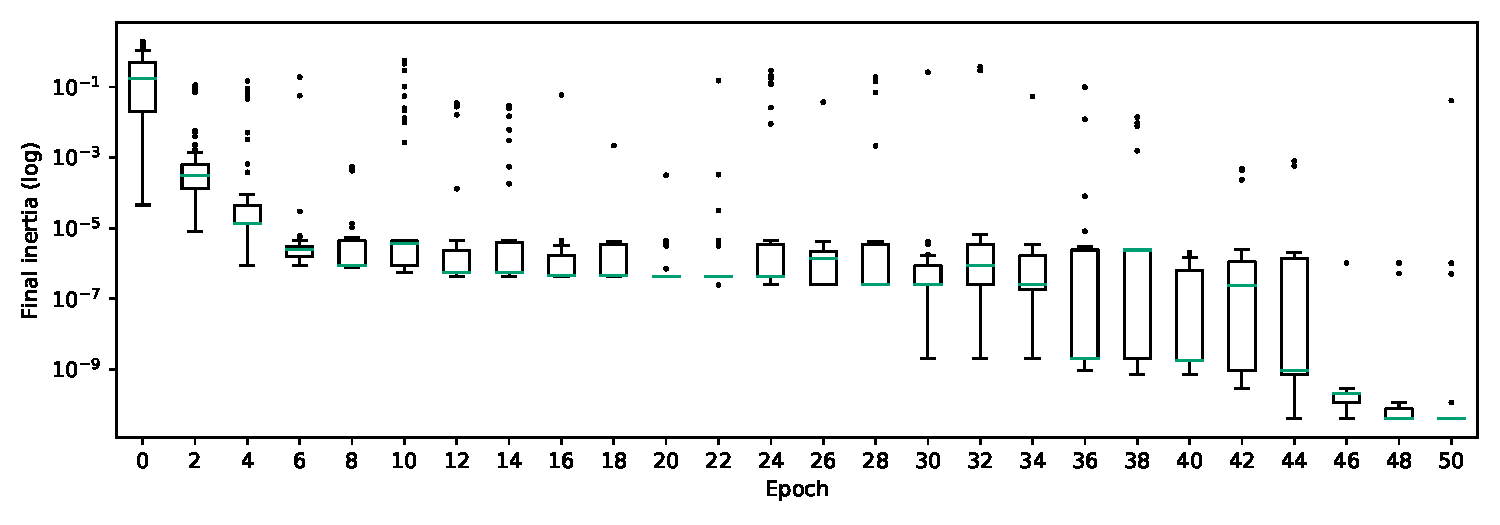
\includegraphics[width=\linewidth]{Fig7a-1.pdf}
        \caption{}\label{fig:edo:inertia:small:fitness}
    \end{subfigure}

    \begin{subfigure}{\imgwidth}
        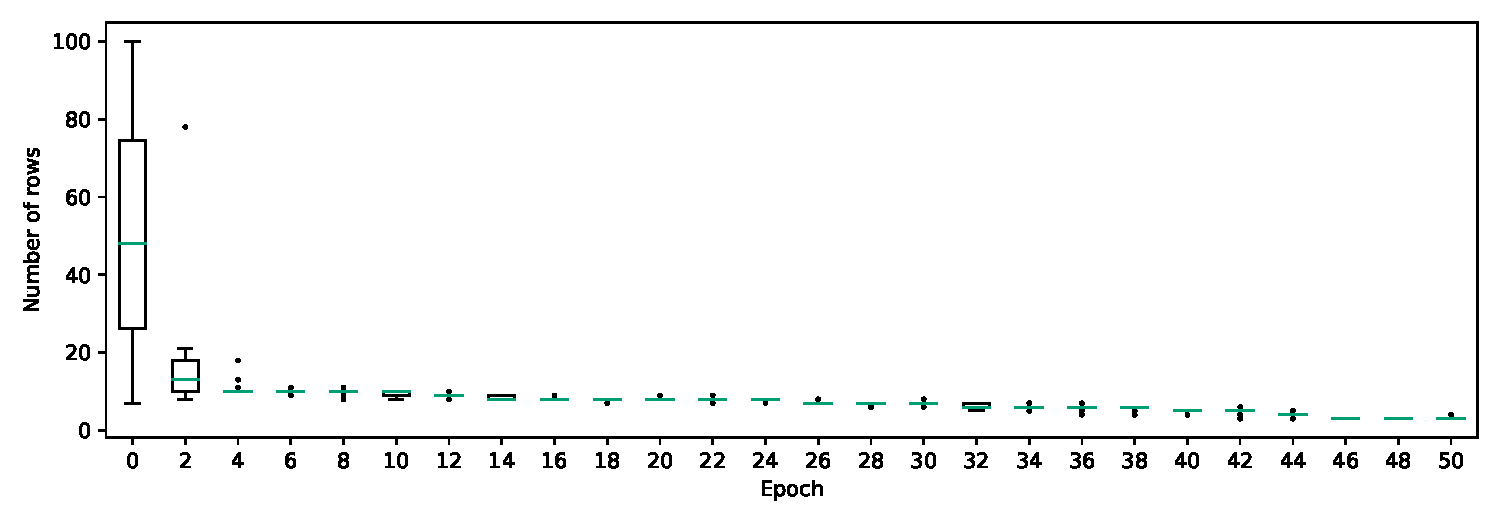
\includegraphics[width=\linewidth]{Fig7a-2.pdf}
        \caption{}\label{fig:edo:inertia:small:dimension}
    \end{subfigure}
    \caption{%
        Progressions for final inertia and dimension across the first 50
        epochs with \(R~=~(3,100)\).
    }\label{fig:small-inertia-50}
\end{figure}

\begin{figure}[htbp]
    \centering
    \begin{subfigure}{\imgwidth}
        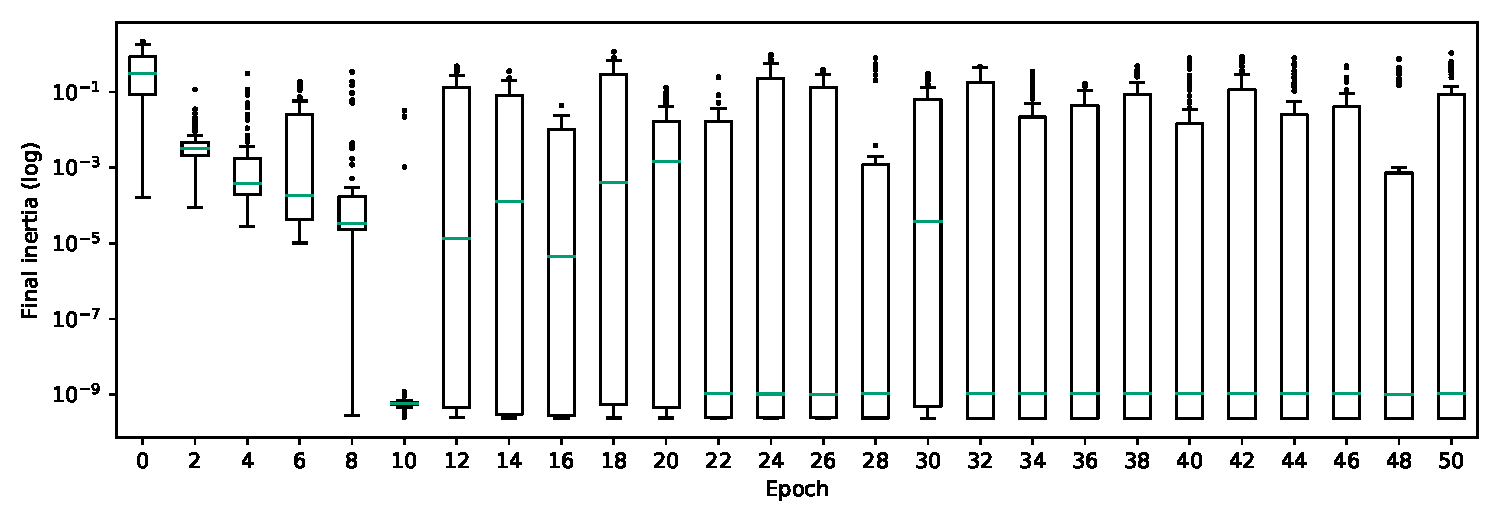
\includegraphics[width=\linewidth]{Fig7b-1.pdf}
        \caption{}\label{fig:edo:inertia:large:fitness}
    \end{subfigure}

    \begin{subfigure}{\imgwidth}
        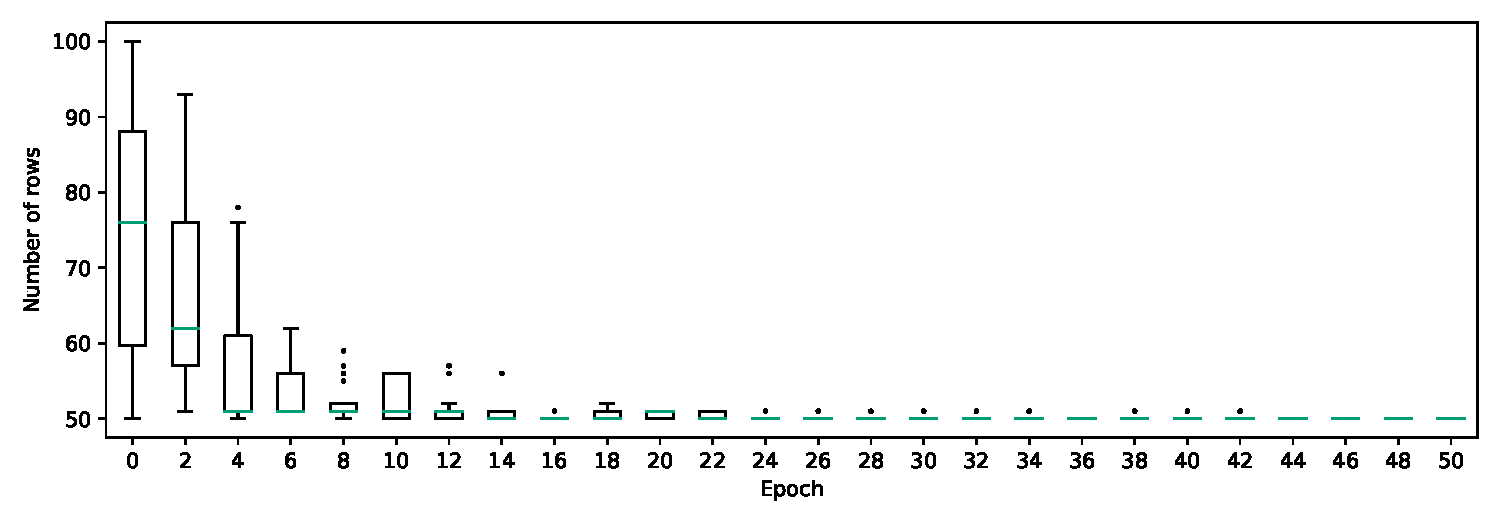
\includegraphics[width=\linewidth]{Fig7b-2.pdf}
        \caption{}\label{fig:edo:inertia:large:dimension}
    \end{subfigure}
    \caption{%
        Progressions for final inertia and dimension across the first 50 epochs
        with \(R~=~(50,100)\).
    }\label{fig:large-inertia-50}
\end{figure}

However, something that may be seen as unwanted is a compaction of the cluster
centres. Referring to Figure~\ref{fig:small-inertia-inds}, the best and median
individuals show two clusters that are essentially the same point whereas the
worst is a random cloud across the whole of \(\mathcal{U}\) which was found in
the initial population. The kind of behaviour exhibited by the best performing
individuals here occurs in part because it is allowed. There are two immediate
ways in which this allowed: first, that a near-trivial case is included in \(R\)
and, secondly, that the fitness function does nothing to penalise the proximity
of the inter-cluster means, as well as aiming to reduce the intra-cluster means.
This kind of unwanted behaviour highlights a subtlety in how EDO should be used;
that experimentation and rigour are required to properly understand an
algorithm's quality.

\begin{figure}[htbp]
    \centering
    \begin{subfigure}{\imgwidth}
        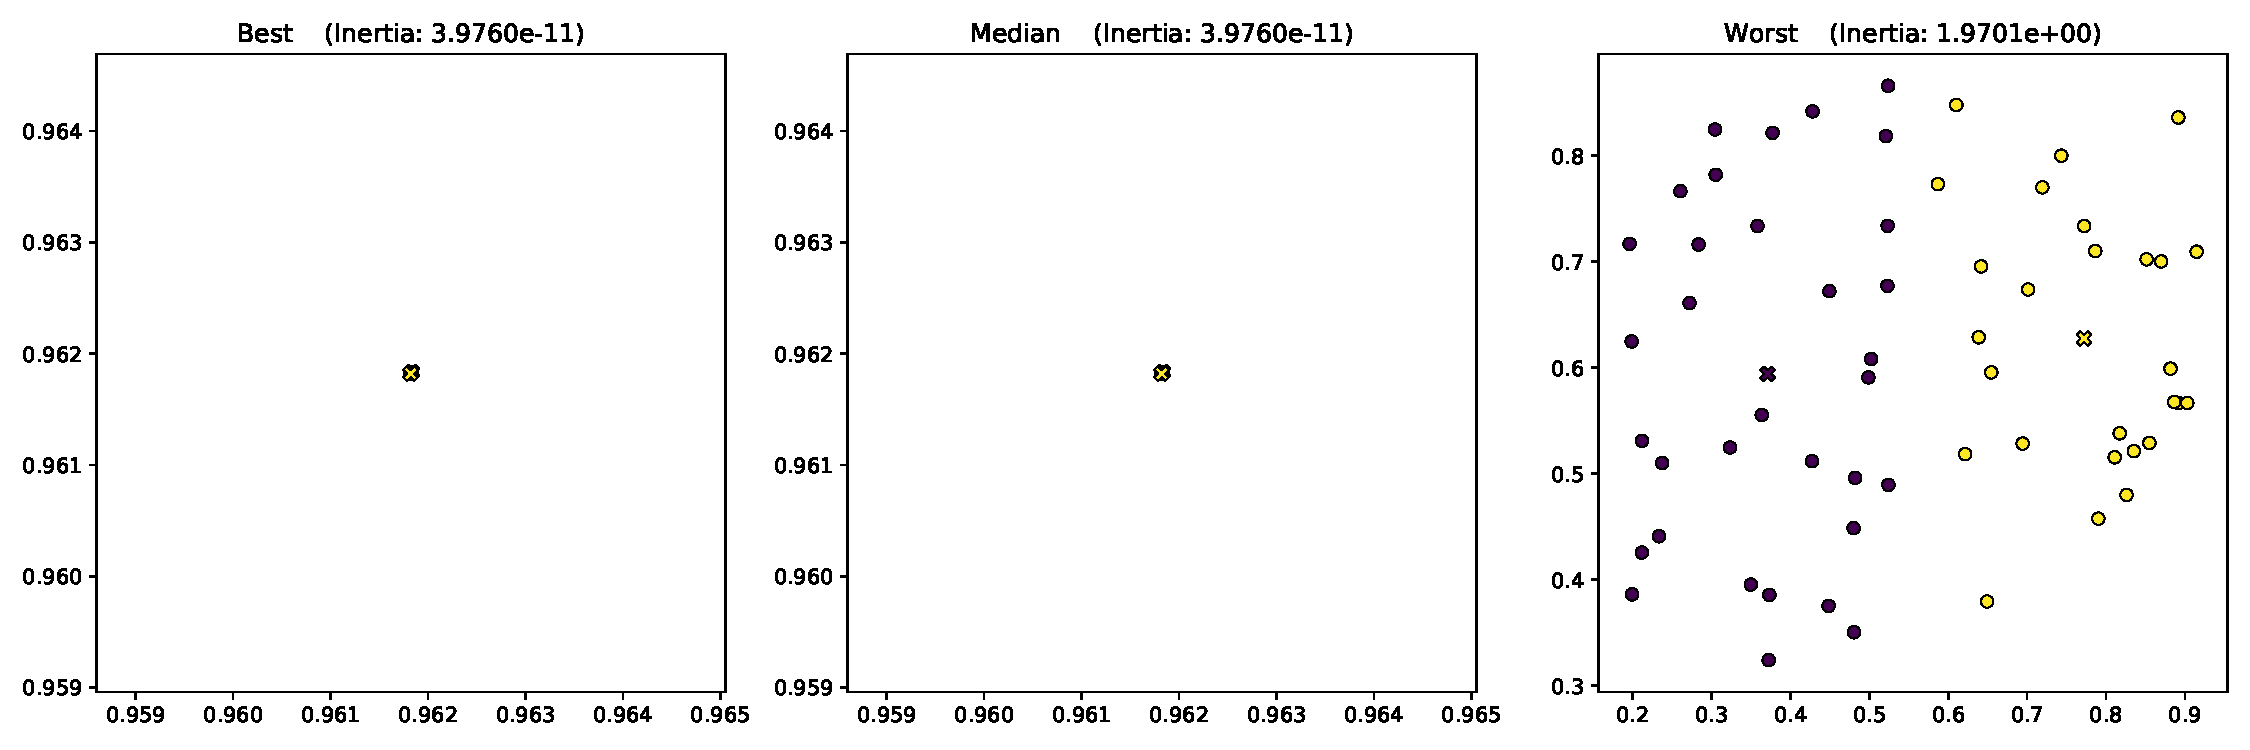
\includegraphics[width=\linewidth]{Fig8a.pdf}
        \caption{}\label{fig:small-inertia-inds}
    \end{subfigure}

    \begin{subfigure}{\imgwidth}
        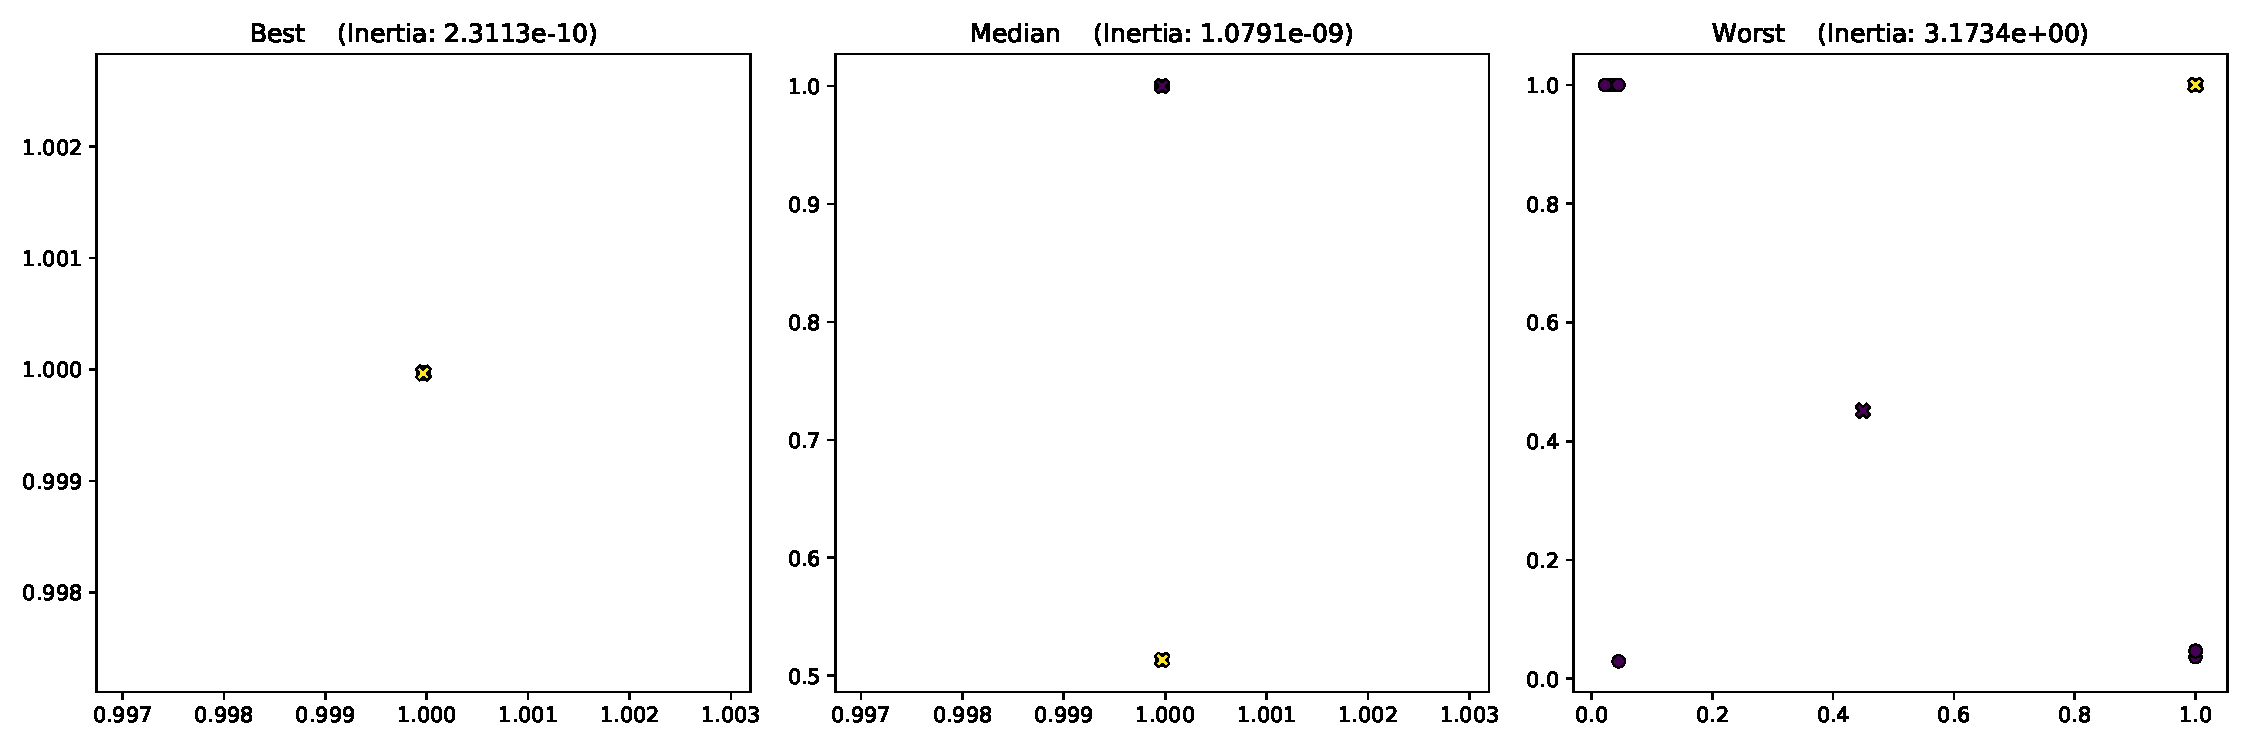
\includegraphics[width=\linewidth]{Fig8b.pdf}
        \caption{}\label{fig:large-inertia-inds}
    \end{subfigure}
    \caption{%
        Representative individuals based on inertia with:
        \subref{fig:small-inertia-inds} \(R~=~(3,100)\);
        \subref{fig:large-inertia-inds} \(R~=~(50,100)\). Centroids displayed as
        crosses.
    }\label{fig:inertia-inds}
\end{figure}

Hence, consider Figure~\ref{fig:large-inertia-inds} where the individuals have
been generated with the same parameters as previously except with adjusted row
limits, \(R = (50, 100)\), so as to exclude this trivial case. In these trials,
the results are equivalent: the worst performing individuals are without
structure whilst the best-performing individuals display clusters that are dense
about a single point despite the minimum number of rows being increased.
Supposing this was not already a known result, we can see mounting evidence in
favour of this compaction being `optimal' behaviour in a dataset for \(k\)-means
clustering.

However, the fitness function may be addressed still, and more extensive
studying may be done. Indeed, the final inertia could be considered a flawed or
fragile fitness function if it is supposed to evaluate the efficacy of the
\(k\)-means algorithm. Incorporating the inter-cluster spread to the fitness
of an individual dataset would reduce this observed compaction. For instance,
the silhouette coefficient is a metric used to evaluate the appropriateness of a
clustering to a dataset and does precisely that. The silhouette coefficient of a
clustering of a dataset is given by the mean of the silhouette value,
\(S(x)\), of each point \(x \in Z_j\) in each cluster:
\begin{equation}
    \begin{gathered}
        A(x) := \frac{1}{|Z_j| - 1} \sum_{y \in Z_j \setminus \{x\}} d(x, y),
        \\
        B(x) := \min_{k \neq j} \frac{1}{|Z_k|} \sum_{w \in Z_k} d(x, w),
        \\
        S(x) :=
            \begin{cases}
                \frac{B(x) - A(x)}{\max\left\{A(x), B(x)\right\}}
                &\quad \text{if } |Z_j| > 1\\
                0 &\quad \text{otherwise}
            \end{cases}
    \end{gathered}\label{eq:silhouette}
\end{equation}\\

The optimisation of the silhouette coefficient is analogous to finding a dataset
which increases both the intra-cluster cohesion (the inverse of \(A\)) and
inter-cluster separation (\(B\)). Hence, the objective of minimising inertia is
addressed by maximising cohesion. Meanwhile, the additional desire to spread out
the clusters is considered by maximising separation.

Repeating the trials with the same parameters as with inertia, the silhouette
fitness function yields the results summarised in
Figures~\ref{fig:small-silhouette}~and~\ref{fig:large-silhouette}. Irrespective
of row limits, the datasets produced show increased separation from one another
whilst maintaining low values in the final inertia of the clustering as shown in
Figure~\ref{fig:silhouette-inds}. Again, the form of the individual clusters is
much the same. The low values of inertia correspond to tight clusters, and the
tightest clusters are those with a minimal number of points, i.e.\ a single
point. As with the previous example, albeit at a much slower rate, the
preferable individuals are those leading toward this case. That this gradual
reduction in the dimension of the individuals occurs despite adjusting the
fitness function and considering the space which excludes the trivial case
bolsters the claim that the base case is also optimal.

At this point, it should be noted that, due to the nature of the implementation,
any individual from any generation may be retrieved and studied should the final
results be too concentrated on any given case. The summary provided here is one
particular way of studying the body of datasets generated with this method and
this transparency in the history and progression of the proposed method is
something that sets it apart from other methods such as GANs which have a
reputation of providing so-called `black box' solutions.

\begin{figure}[htbp]
    \centering
    \begin{subfigure}{\imgwidth}
        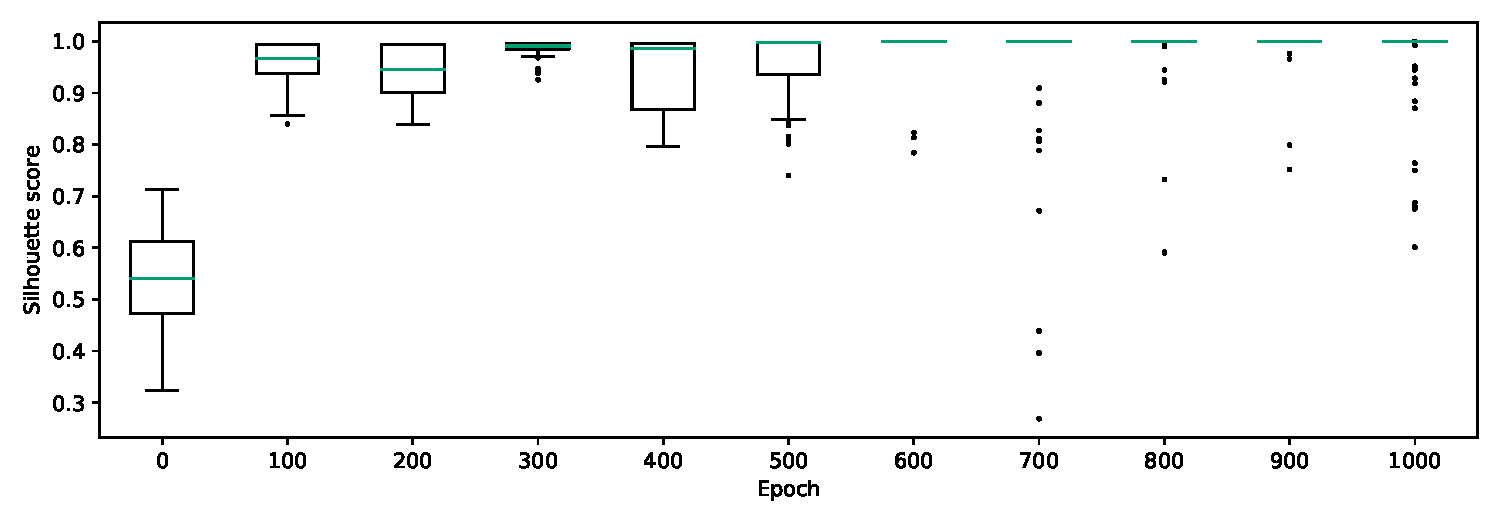
\includegraphics[width=\linewidth]{Fig9a-1.pdf}
        \caption{}\label{fig:edo:small:silhouette}
    \end{subfigure}

    \begin{subfigure}{\imgwidth}
        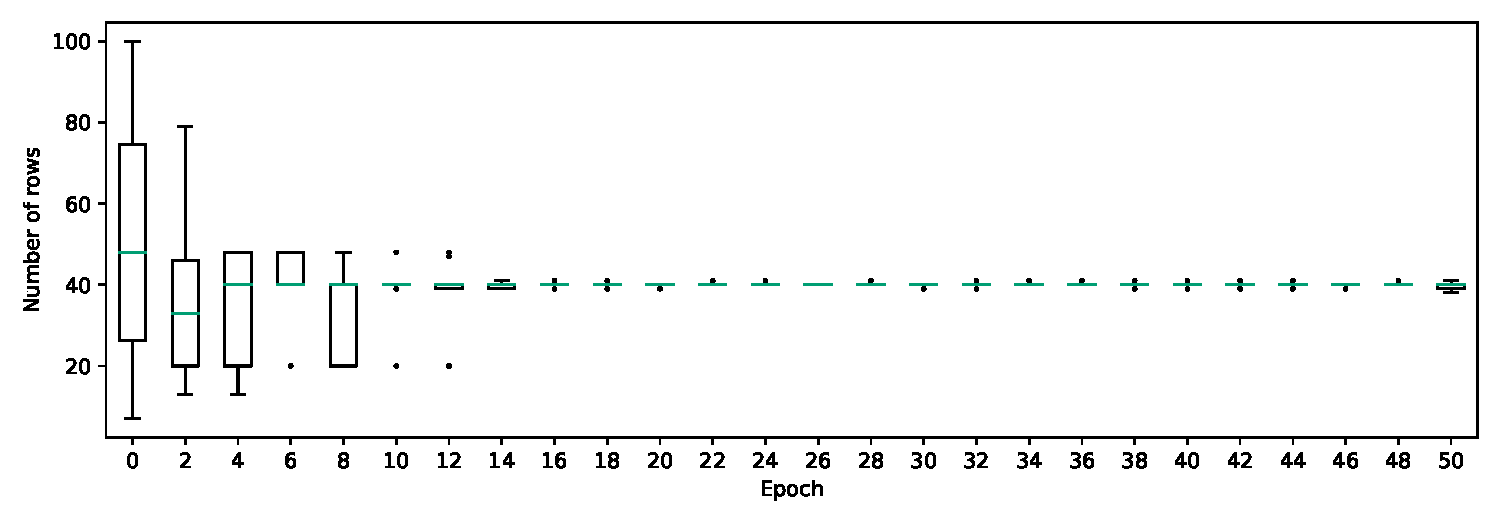
\includegraphics[width=\linewidth]{Fig9a-2.pdf}
        \caption{}\label{fig:edo:small:dimension}
    \end{subfigure}
    \caption{%
        Progressions of silhouette and dimension across 1000 epochs at 100 epoch
        intervals with \(R~=~(3, 100)\).
    }\label{fig:small-silhouette}
\end{figure}

\begin{figure}
    \centering
    \begin{subfigure}{\imgwidth}
        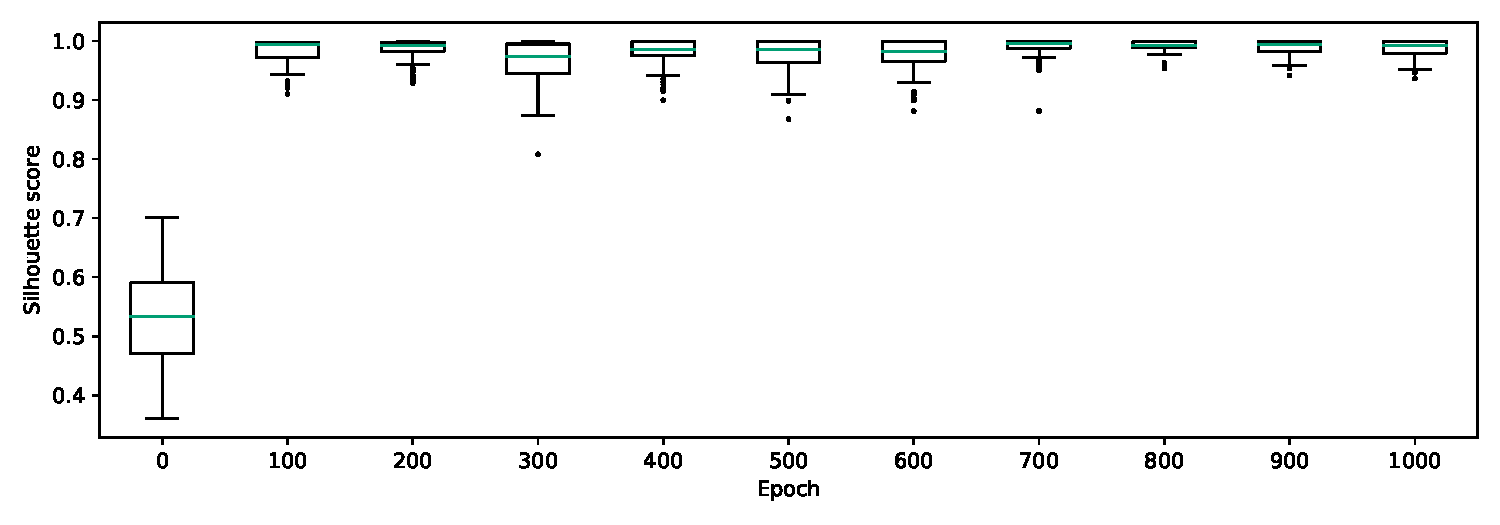
\includegraphics[width=\linewidth]{Fig9b-1.pdf}
        \caption{}\label{fig:edo:large:silhouette}
    \end{subfigure}

    \begin{subfigure}{\imgwidth}
        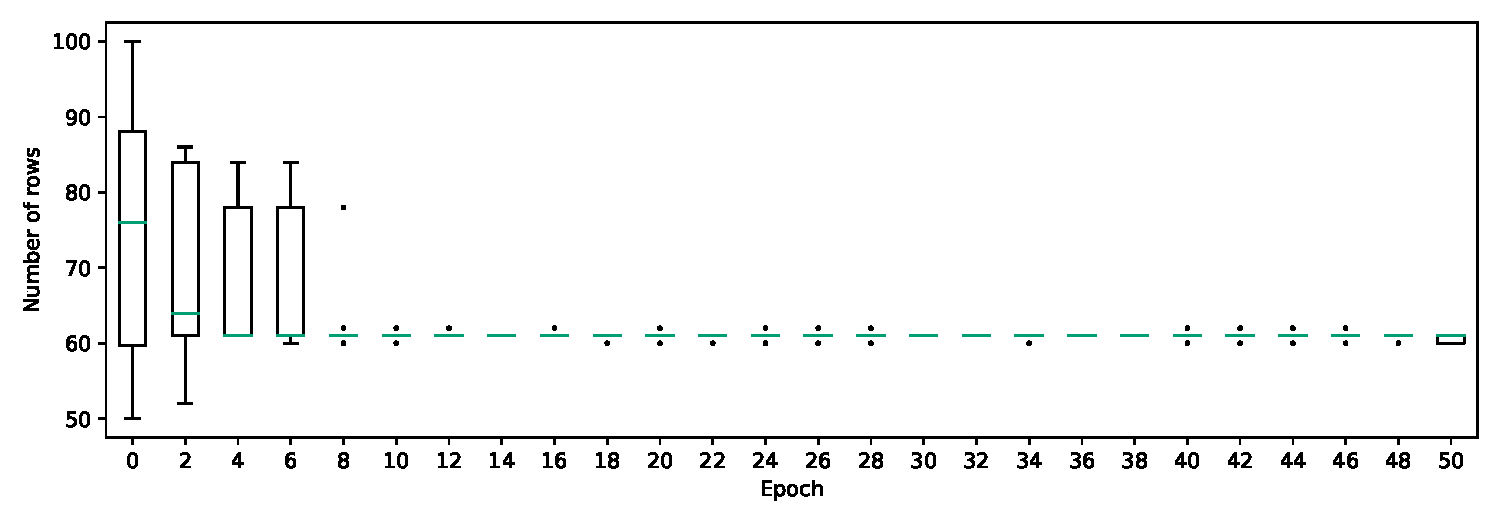
\includegraphics[width=\linewidth]{Fig9b-2.pdf}
        \caption{}\label{fig:edo:large:dimension}
    \end{subfigure}
    \caption{%
        Progressions of silhouette and dimension across 1000 epochs at 100 epoch
        intervals with \(R~=~(50,100)\).
    }\label{fig:large-silhouette}
\end{figure}

\begin{figure}
    \centering
    \begin{subfigure}{\imgwidth}
        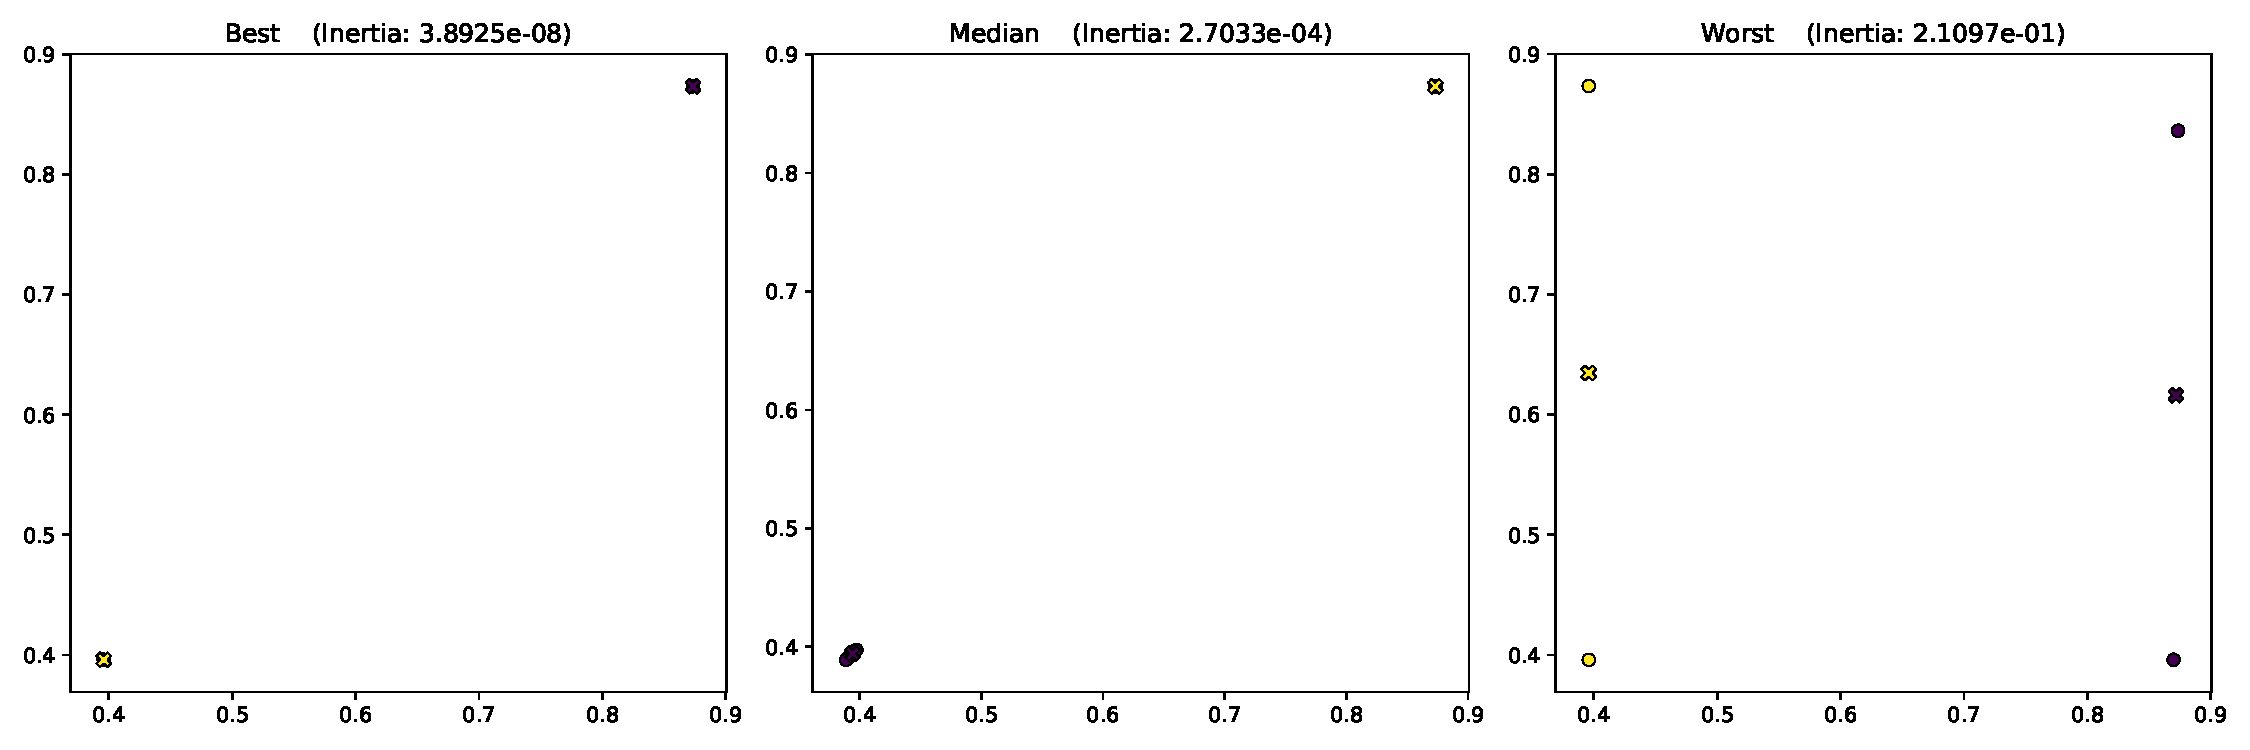
\includegraphics[width=\linewidth]{Fig10a.pdf}
        \caption{}\label{fig:edo:small:silhouette:inds}
    \end{subfigure}

    \begin{subfigure}{\imgwidth}
        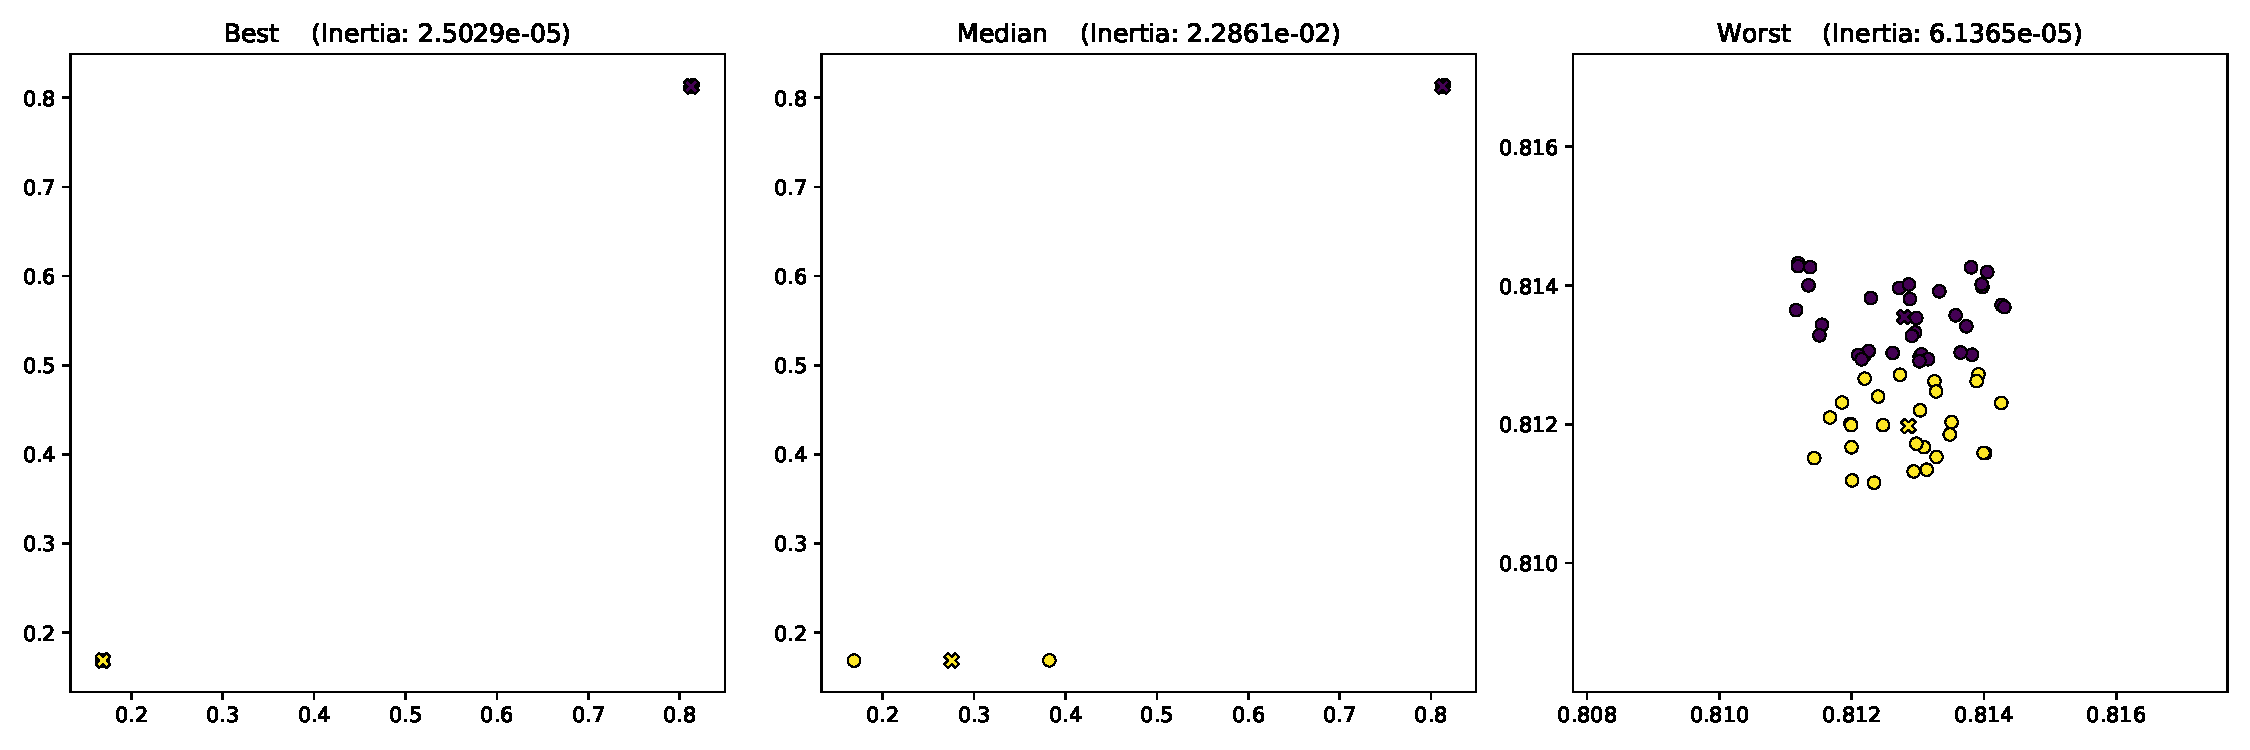
\includegraphics[width=\imgwidth]{Fig10b.pdf}
        \caption{}\label{fig:edo:large:silhouette:inds}
    \end{subfigure}
    \caption{%
        Representative individuals based on silhouette with:
        \subref{fig:edo:small:silhouette:inds} \(R~=~(3,100)\);
        \subref{fig:edo:large:silhouette:inds} \(R~=~(50,100)\). Centroids are
        displayed as crosses.
    }\label{fig:silhouette-inds}
\end{figure}

\subsection{Comparison with DBSCAN}\label{subsec:dbscan}

The extent of the capabilities EDO holds as a tool to better understand an
algorithm are especially apparent when comparing an algorithm against another
(or set of others) simultaneously. This is done by utilising the freedom of
choice in a fitness function for EDO.\ Consider two algorithms, \(A\) and \(B\),
and some common metric between them, \(g\). Then their similarities and
contrasts can be explored by considering the differences in this metric on the
two algorithms. In terms of EDO, this means using \(f = g_A - g_B\), \(f = g_B -
g_A\) or \(f = \left| g_B - g_A \right|\) as the fitness function. By doing so,
pitfalls, edge cases or fundamental conditions for the method may be
highlighted. Overall, this process allows the researcher to more deeply learn
about the method of interest beyond the traditional method of literature
comparison on a particular example.

Consider the following use case with another clustering algorithm of a different
form, Density Based Spatial Clustering of Applications with Noise (DBSCAN). In
this particular case, the objective is to find datasets for which the method of
interest, \(k\)-means, outperforms its alternative, DBSCAN.\ Here there is no
concept of inertia as DBSCAN is density-based and is able to identify
outliers~\cite{Ester1996}. As such, a valid metric must be chosen. One such
metric is the silhouette score as defined in~(\ref{eq:silhouette}).

In this case, however, an adjustment to the fitness function must be made so as
to accommodate for the condition of the silhouette coefficient that there must
be more than one cluster present. Let \(S_k (X)\) and \(S_D (X)\) denote the
silhouette coefficients of the clustering found by \(k\)-means and DBSCAN
respectively. Then the fitness function is defined to be:
\begin{equation}
    f(X) =
        \begin{cases}
            S_D (X) - S_k (X), &\quad \text{%
                \begin{tabular}{l}%
                    if DBSCAN identifies two or
                    \\
                    more clusters (inc.\ noise)
                \end{tabular}
            }\\
            \infty &\quad \ \ \text{otherwise.}
        \end{cases}\label{eq:dbscan-fitness}
\end{equation}

There are several remarks to be made here. First, note the order of the
subtraction here as EDO minimises fitness functions by default. Also, \(f\)
takes values in the range \([-2, 2]\) where \(-2\) is the best, i.e.\ \(S_D(X) =
-1\) and \(S_k(X) = 1\). Likewise, 2 is the worst score. Finally, the silhouette
coefficient requires at least two clusters to be present and so if DBSCAN
identifies a single cluster then that individual will be penalised heavily under
this fitness function when, in fact, that clustering may be of high quality. As
such, this fitness function may require adjustment.

It must also be acknowledged that \(k\)-means and DBSCAN share no common
parameters and so direct comparison is more difficult. For the purposes of this
example, only one set of parameters is used but a thorough investigation should
include a parameter sweep in similar, real-world use cases. The parameters being
used are \(k~=~3\) for \(k\)-means, and \(\epsilon~=~0.1,\ MinPoints~=~5\) for
DBSCAN.\ This set was chosen following informal experimentation using the Python
library Scikit-learn~\cite{scikit} to find comparable parameters in the given
search space defined by the EDO parameters used previously with
\(R~=~(50,100)\).

\begin{figure}
    \centering
    \begin{subfigure}{\imgwidth}
        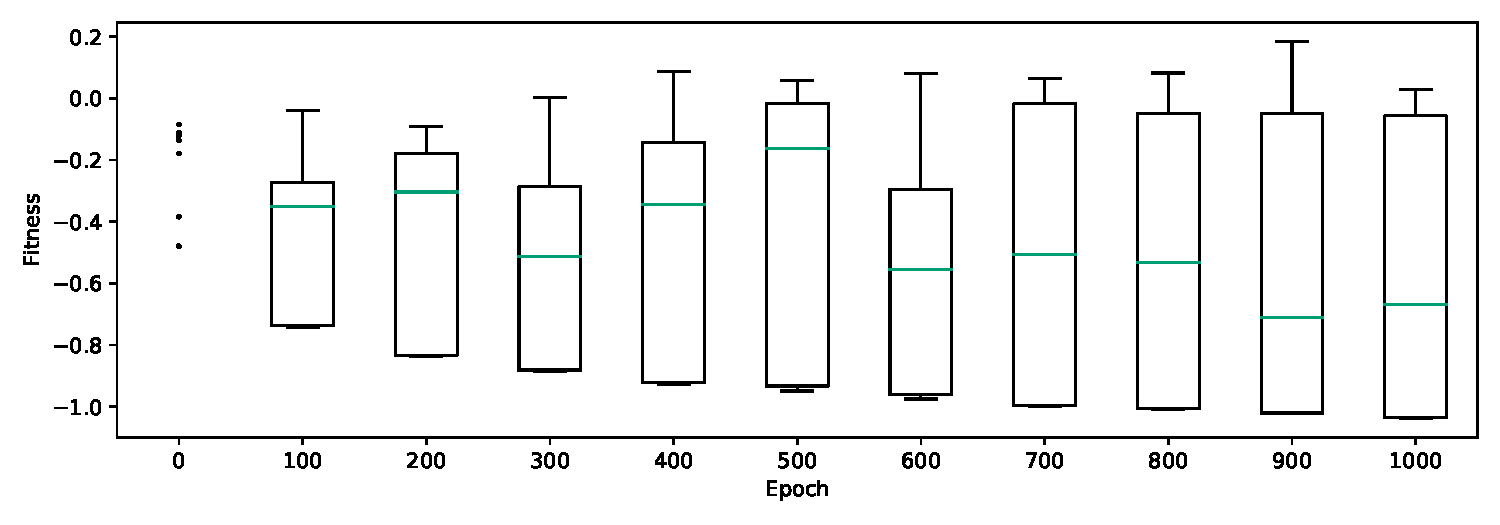
\includegraphics[width=\linewidth]{Fig11-1.pdf}
        \caption{}\label{fig:edo:positive:silhouette}
    \end{subfigure}

    \begin{subfigure}{\imgwidth}
        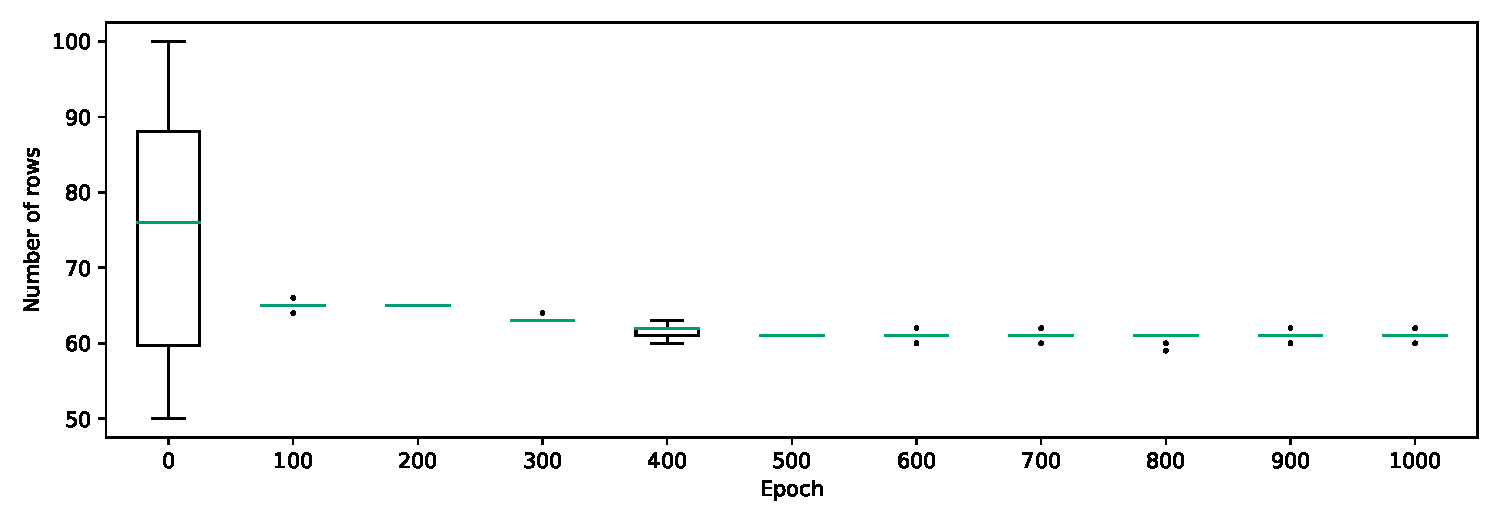
\includegraphics[width=\linewidth]{Fig11-2.pdf}
        \caption{}\label{fig:edo:positive:dimension}
    \end{subfigure}
    \caption{%
        Progressions for difference in silhouette (\(k\)-means-preferable) and
        dimension across 1000 epochs at 100 epoch intervals.
    }\label{fig:dbscan-silhouette}
\end{figure}

\begin{figure}
    \centering
    \begin{subfigure}{\imgwidth}
        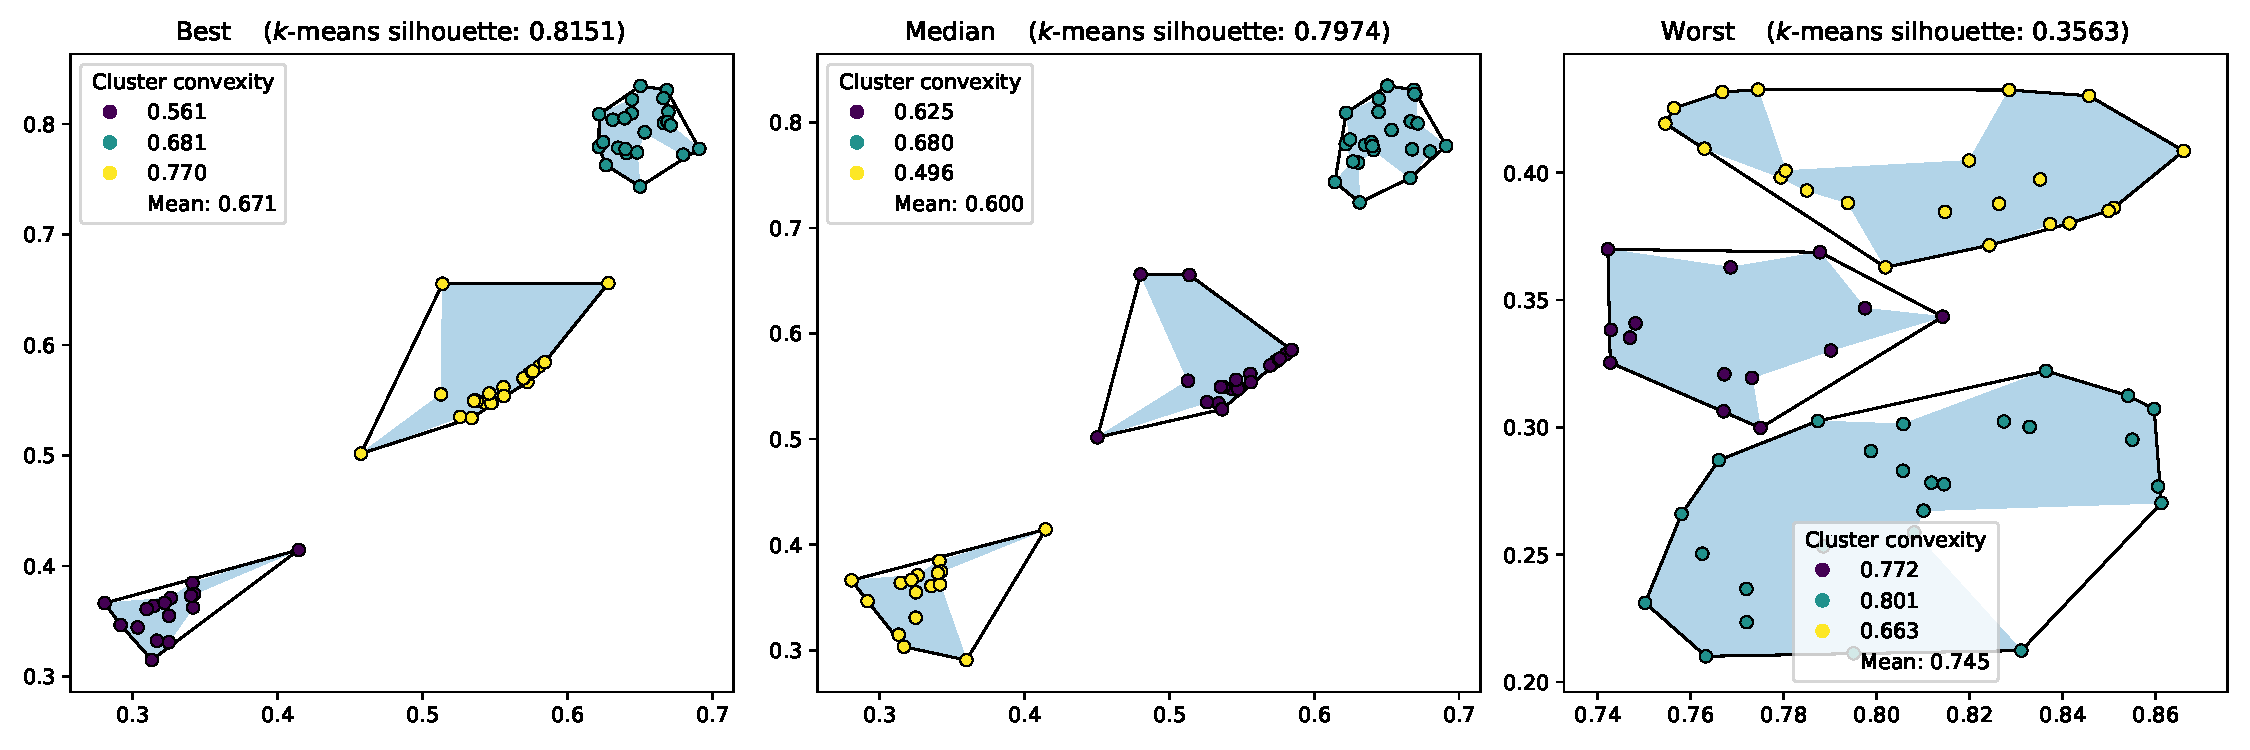
\includegraphics[width=\linewidth]{Fig12a.pdf}
        \caption{}\label{fig:dbscan-inds-k}
    \end{subfigure}

    \begin{subfigure}{\imgwidth}
        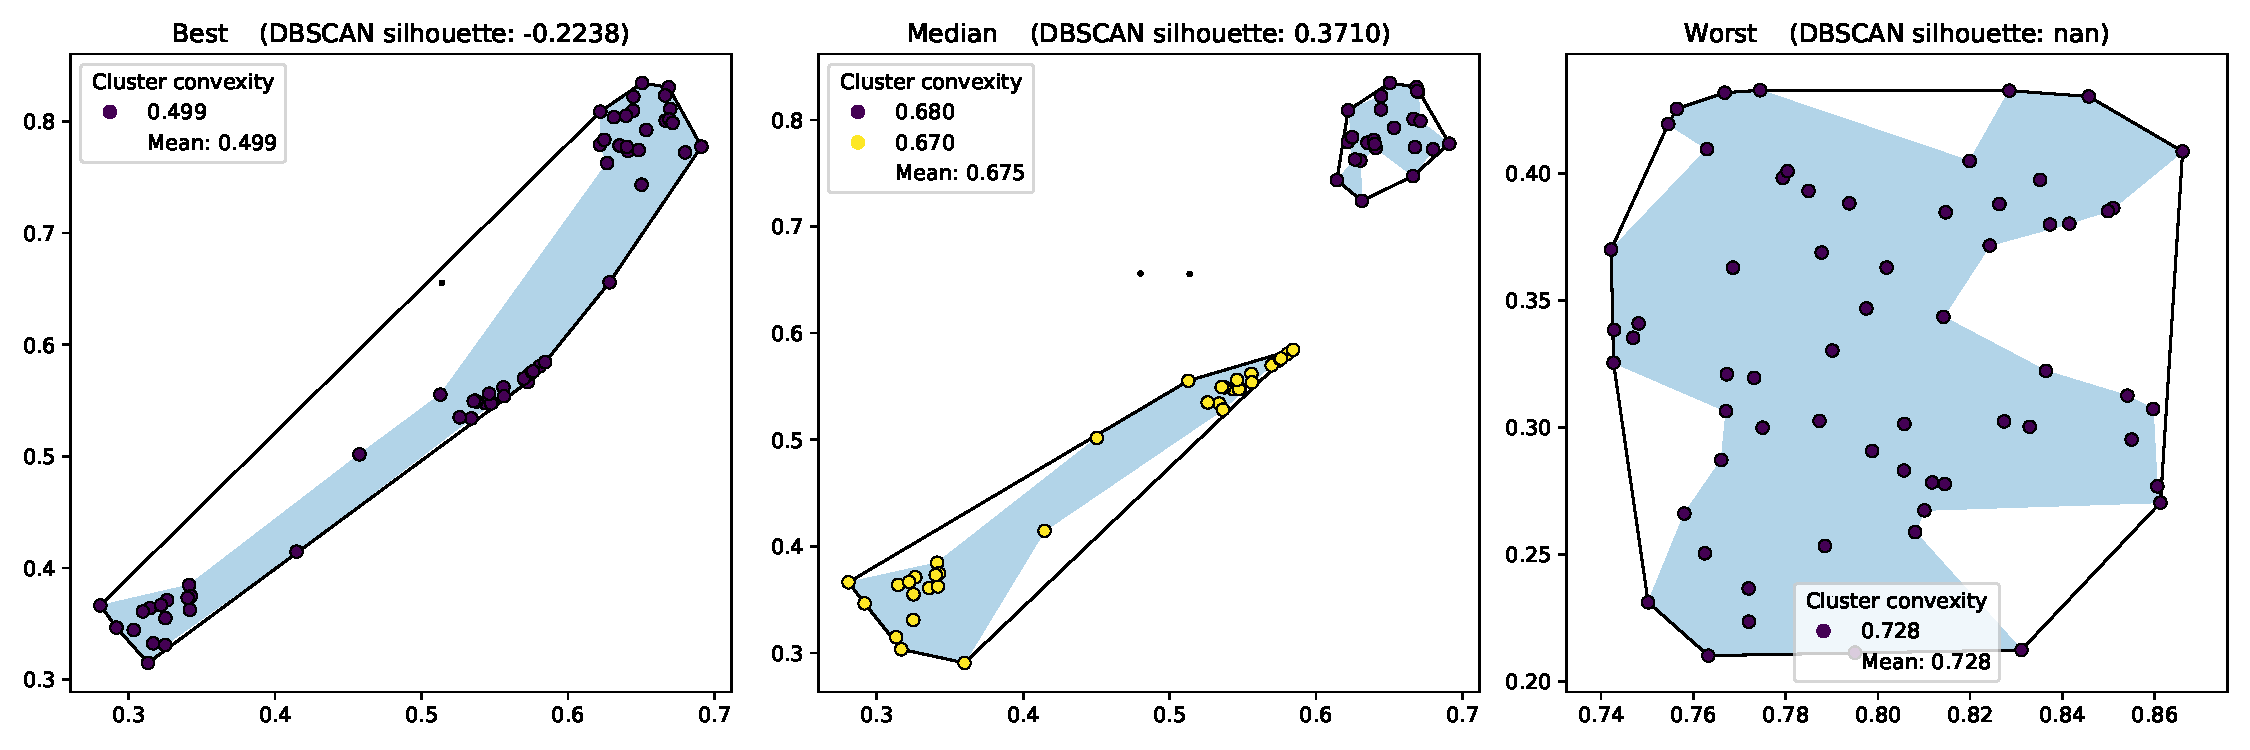
\includegraphics[width=\linewidth]{Fig12b.pdf}
        \caption{}\label{fig:dbscan-inds-d}
    \end{subfigure}
    \caption{%
        Representative individuals from a \(k\)-means-preferable run with
        clustering by: \subref{fig:dbscan-inds-k} \(k\)-means;
        \subref{fig:dbscan-inds-d} DBSCAN.\ Concave and convex hulls illustrated
        by shading and outline respectively.
    }\label{fig:dbscan-inds}
\end{figure}

Figure~\ref{fig:dbscan-silhouette} shows a summary of the progression of EDO
for this use case. As with the previous examples where \(R~=~(50, 100)\), the
variation in the population fitness is unstable but there is a clear trend of
improvement in the best individual over the course of the run. There is also a
convergence seen in the number of rows a dataset has. The resting dimension
varied across the trials conducted in this work but none exhibited a dramatic
shift toward the lower limit of 50 rows as with previous examples. This is
suggestive of a more competitive environment for individuals where slight
changes to an individual can drastically alter their fitness.

The effect of such changes can be seen in Figure~\ref{fig:dbscan-inds} where
representative individuals are shown for this example. Here, the best performing
individual, when clustered by \(k\)-means, shows three clear and nicely
separated clusters. Note that they are not so tightly packed; again, this
suggests that the route to an optimal individual is less clearly defined. In
contrast, when the same dataset is clustered by DBSCAN a single cluster is found
with a single noise point held within the convex hull of the cluster, i.e.\
there are overlapping clusters (since noise points form a single cluster).
Hence, along with the fact that the larger cluster is widely spread, it follows
that the clustering has a relatively small, negative silhouette coefficient.

Another point of interest here is the convexity of the clusters. A known
condition for the success of \(k\)-means is that the presented clusters are of
roughly equal size and are convex. This is due to the overall objective being to
approximate the centroidal Voronoi tessellation~\cite{Du2006}. Without this
condition, up to the correct choice of \(k\), the algorithm will fail to produce
adequate results for either inertia or silhouette. DBSCAN, on the other hand,
does not have this condition and is able to detect non-convex clusters so long
as they are dense enough. Figure~\ref{fig:dbscan-inds} shows the clustering
found by each method and the respective convex and concave hulls of the clusters
found. The `concave hull' of a cluster is taken to be the \(\alpha\)-shape of
the cluster's data points~\cite{Edelsbrunner1983} where \(\alpha\) is determined
to be the smallest value such that all the points in the cluster are contained
in a single polygon. The convexity of cluster \(Z_j\), denoted
\(\mathcal{C}_j\), is then determined to be the ratio of the area of its concave
hull, \(H_c\), to the area of its convex hull, \(H_v\)~\cite{Sonka1993}:
\begin{equation}
    \mathcal{C}_j :=
    \frac{\text{area}\left(H_c\right)}{\text{area}\left(H_v\right)}
\end{equation}

With this definition, it should be clear that a perfectly convex cluster, such
as a single point or line, would have \(\mathcal{C}_j = 1\).

It can be seen that the convexity of the clustering found by \(k\)-means appears
to be higher than that by DBSCAN.\ This was apparent across all trials conducted
in this work and indicates that the condition for convex clusters is being
sought out during the optimisation process. Meanwhile, however, it is not clear
whether the performance of DBSCAN falls owing to its parameters or the method
itself. This is a point where parameter sweeping would prove most useful so as
to determine a crossing point for these two driving forces.

Now, to add to the discussion above, the inverse optimisation should be
considered. That is, using the same parameters, the datasets for which DBSCAN
outperforms \(k\)-means with respect to the silhouette coefficient are to be
investigated. This is equivalent to using \(-f\) as the fitness function
except with the same penalty of \(\infty\) for the case set out
in~(\ref{eq:dbscan-fitness}).

\begin{figure}[htbp]
    \centering
    \begin{subfigure}{\imgwidth}
        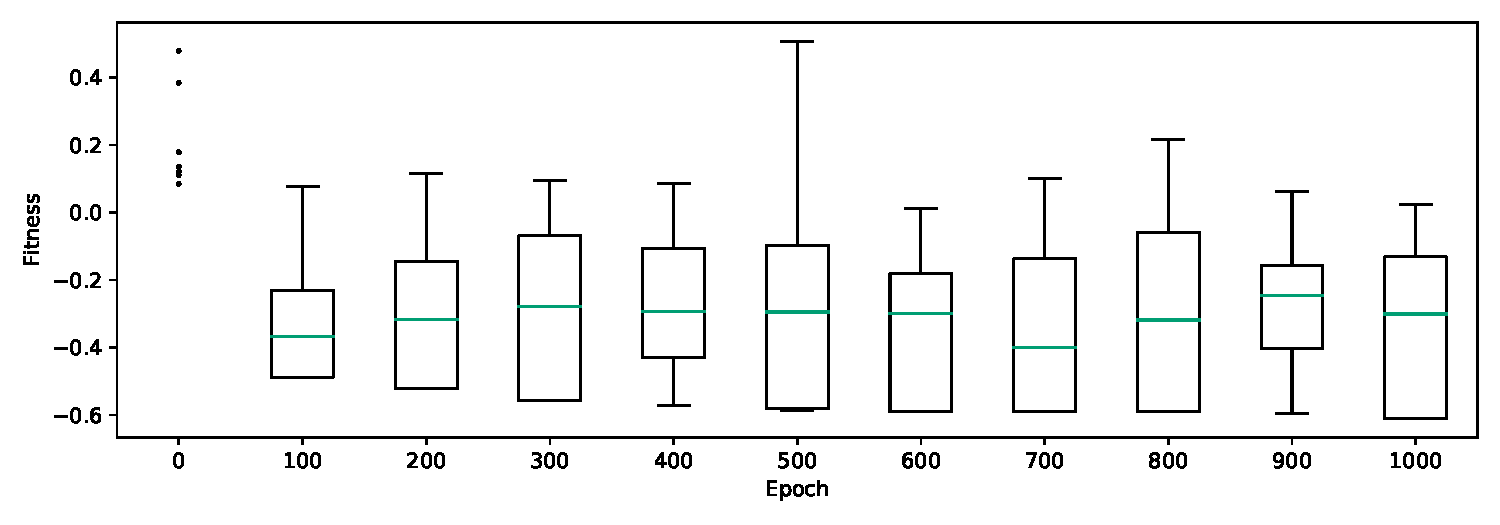
\includegraphics[width=\linewidth]{Fig13-1.pdf}
        \caption{}\label{fig:edo:negative:silhouette}
    \end{subfigure}

    \begin{subfigure}{\imgwidth}
        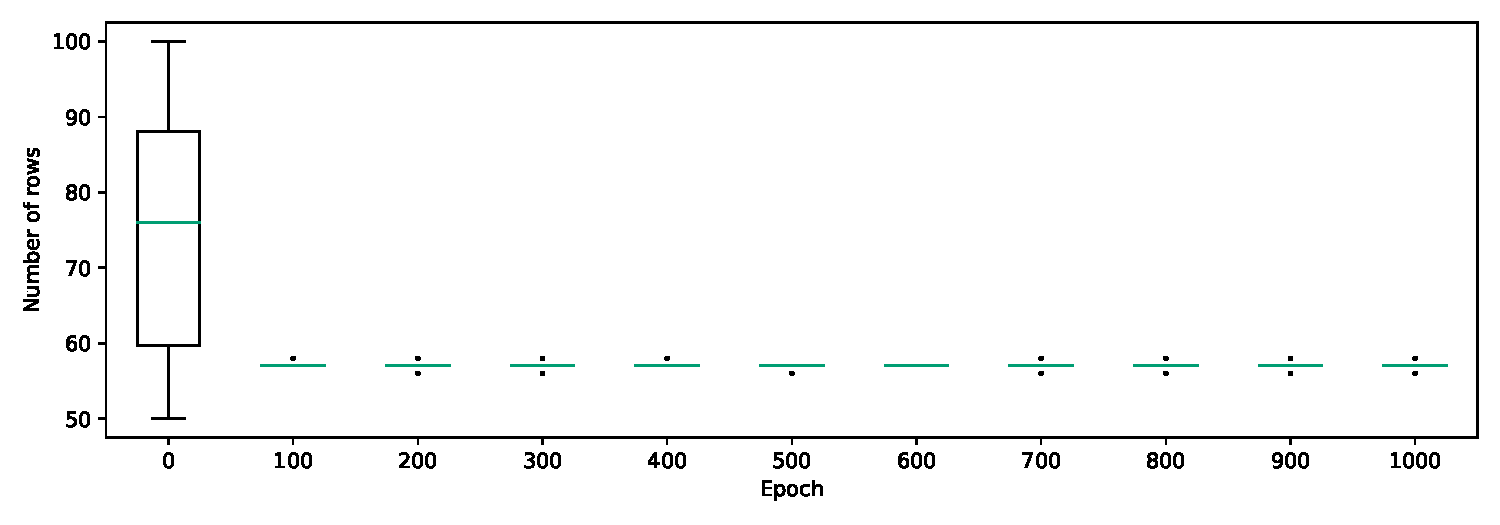
\includegraphics[width=\linewidth]{Fig13-2.pdf}
        \caption{}\label{fig:edo:negative:dimension}
    \end{subfigure}
    \caption{%
        Progressions for difference in silhouette (DBSCAN-preferable) and
        dimension across 1000 epochs at 100 epoch intervals.
    }\label{fig:negative-prog}
\end{figure}

\begin{figure}
    \centering
    \begin{subfigure}{\imgwidth}
        \centering
        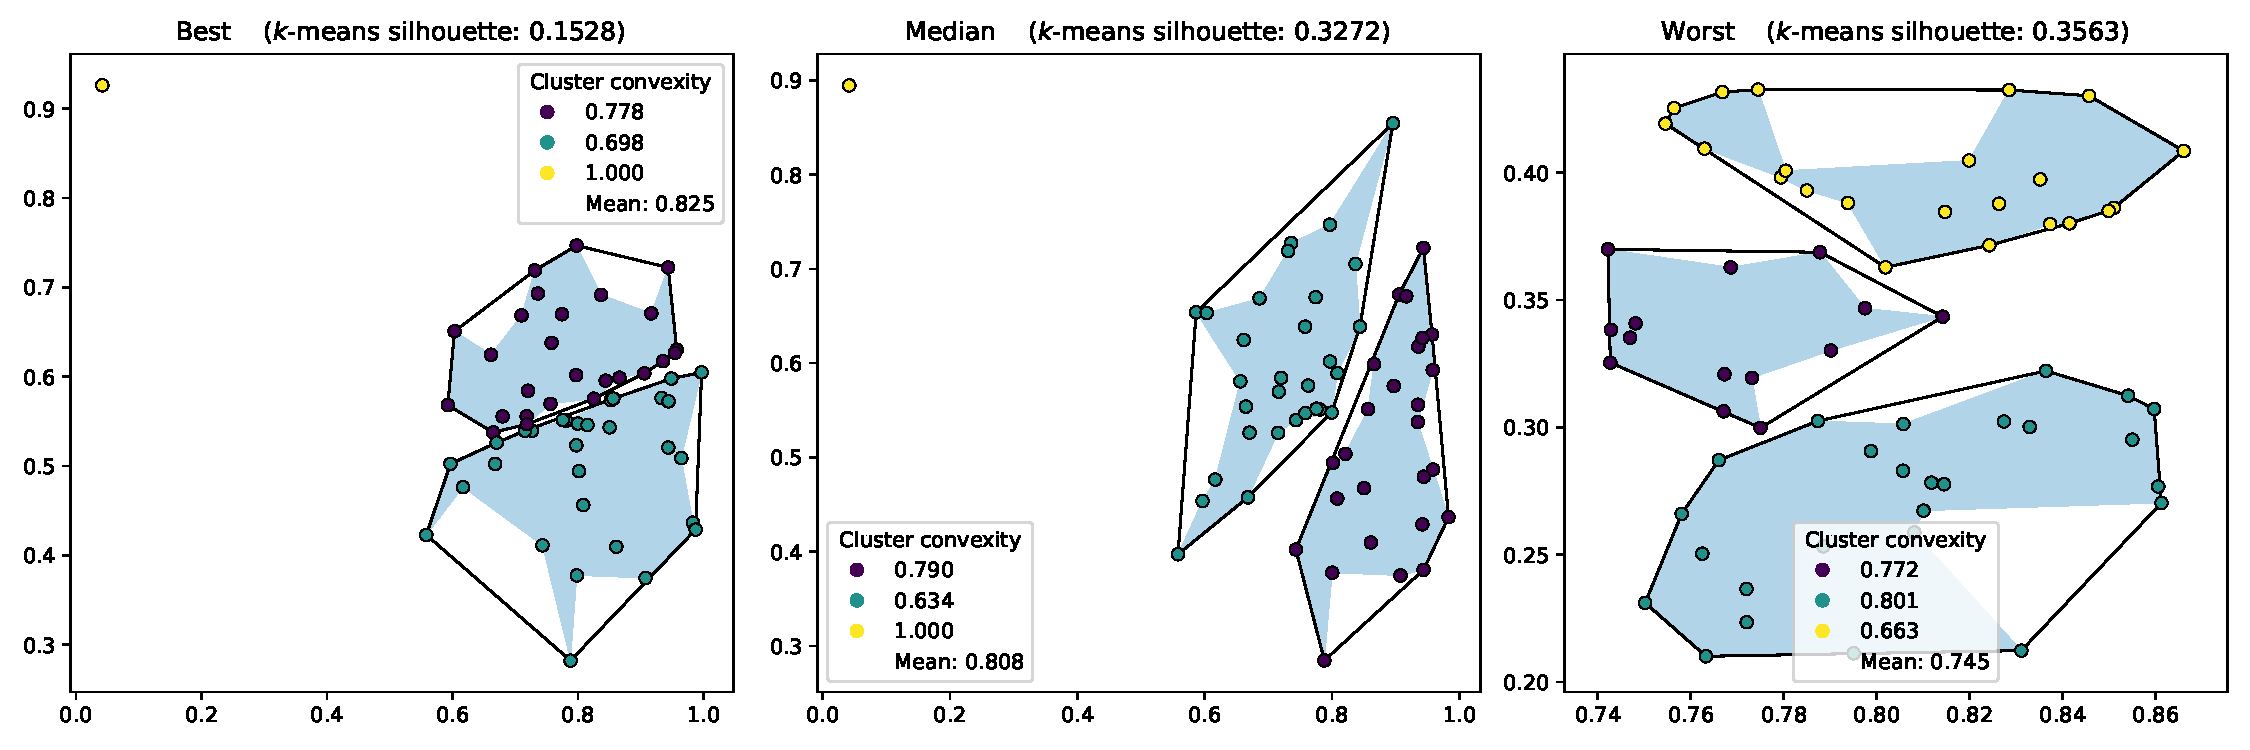
\includegraphics[width=\linewidth]{Fig14a.pdf}
        \caption{}\label{fig:neg-inds-k}
    \end{subfigure}

    \begin{subfigure}{\imgwidth}
        \centering
        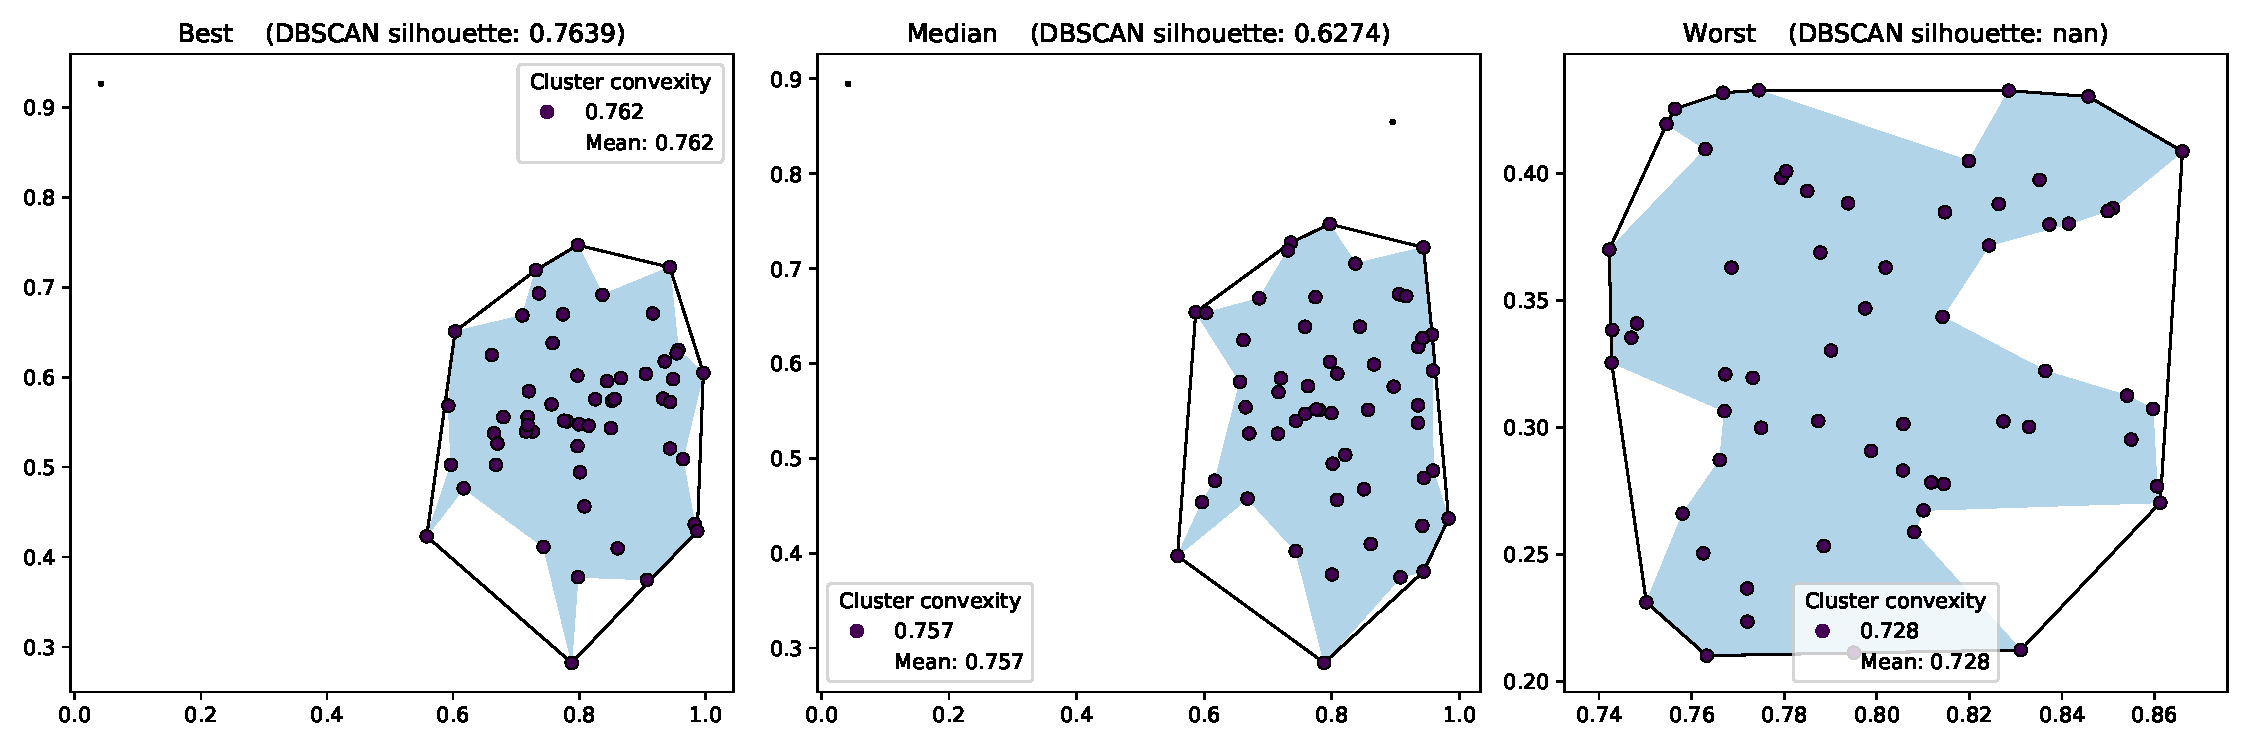
\includegraphics[width=\linewidth]{Fig14b.pdf}
        \caption{}\label{fig:neg-inds-d}
    \end{subfigure}
    \caption{%
        Representative individuals from a DBSCAN-preferable run with clustering
        by: \subref{fig:dbscan-inds-k} \(k\)-means; \subref{fig:dbscan-inds-d}
        DBSCAN.\ Concave and convex hulls illustrated by shading and outline
        respectively.
    }\label{fig:negative-inds}
\end{figure}

Figures~\ref{fig:negative-prog}~and~\ref{fig:negative-inds} show the same
summary as above with the revised fitness function. Inspecting the former, it is
seen that the best fitness found is worse than with the previous example. This,
in part, is due to the fact that \(k\)-means cannot find a clustering with
negative values as no clusters may overlap. It can, however, produce results
with small silhouette scores where the clusters are tightly packed. Hence, the
best fitness score is now \(-1\) whereas the worst is 2, still.

Note in the first two frames of Figure~\ref{fig:neg-inds-k} how \(k\)-means is
forced to split what is evidently a single cluster in two whereas DBSCAN is able
to identify the single cluster and the outlying noise
(Figure~\ref{fig:neg-inds-d}). The proximity of these clusters has then dragged
the silhouette score down for \(k\)-means. Referring to
Figure~\ref{fig:neg-inds-d}, this kind of behaviour is certainly preferable for
DBSCAN under these parameters: the beginning individuals are likely random
clouds (as seen in the rightmost two frames of the figure) and the simplest step
toward a fit dataset is one that maintains that vaguely dense body with minimal
noise points far from it.

As has already been stated, the software implementation of the EDO method
has been produced in line with the best practices of open source software
development and reproducible research. In aid of this, all of the source code
used in these examples (including to create the figures) has been archived
under the DOI
\href{https://doi.org/10.5281/zenodo.3492236}{10.5281/zenodo.3492236}.
Likewise, all of the data produced to support this case study have been archived
under the DOI
\href{https://doi.org/10.5281/zenodo.3492228}{10.5281/zenodo.3492228}.


\section{Conclusion}

In this paper we have introduced a novel approach to understanding the quality
of an algorithm by exploring the space in which their well-performing datasets
exist. Following a detailed explanation of its internal mechanisms, a case study
in \(k\)-means clustering was offered as validation for the proposed method.
The method was able to reveal some known results without prior knowledge when
investigating \(k\)-means in several scenarios, and again when comparing
\(k\)-means and another leading clustering method, DBSCAN.\

The method itself utilises biological operators to traverse a potentially broad
region of the space of all possible datasets. This is done in an organic way
with a minimal external framework attached. The generative nature of the
proposed method also provides transparency and richness to the solution when
compared to other contemporary techniques for artificial data generation as the
entire history of individuals is preserved. While other search and optimisation
methods exist, the decision to use an EA here was down to this transparency and
the ease with which to implement biological operators that are both meaningful
and easily understood.

The Evolutionary Dataset Optimisation method is dependent on a number of
parameters set out in this work one of which is the choice of distribution
families, \(\mathcal{P}\); these families go on to define the general
statistical shape of the columns of the datasets that are produced and also
control the present data types. The relationship between columns and their
associated distribution is not causal and appropriate methods should be employed
to understand the structure and characteristics of the data produced before
formal conclusions are made as set out in the case study provided.

It is known that EAs might terminate at a local optimum and may not be able to
traverse the entire sample space~\cite{Vikhar2016}, or even a sufficient part of
it. This would be even more problematic in the case presented in this work where
the sample space is not even of a fixed size or data type. In all experiments
carried out for this work, this theoretic limitation has not arisen.
Figure~\ref{fig:coverage} shows an exploration of the sample space and it is
evident that the EDO method was able to explore a large proportion of it. In the
early stages, it is also clear here how the EA got stuck in small parts of the
search space before later moving toward a subregion of the unit square.

\begin{figure}[htbp]
    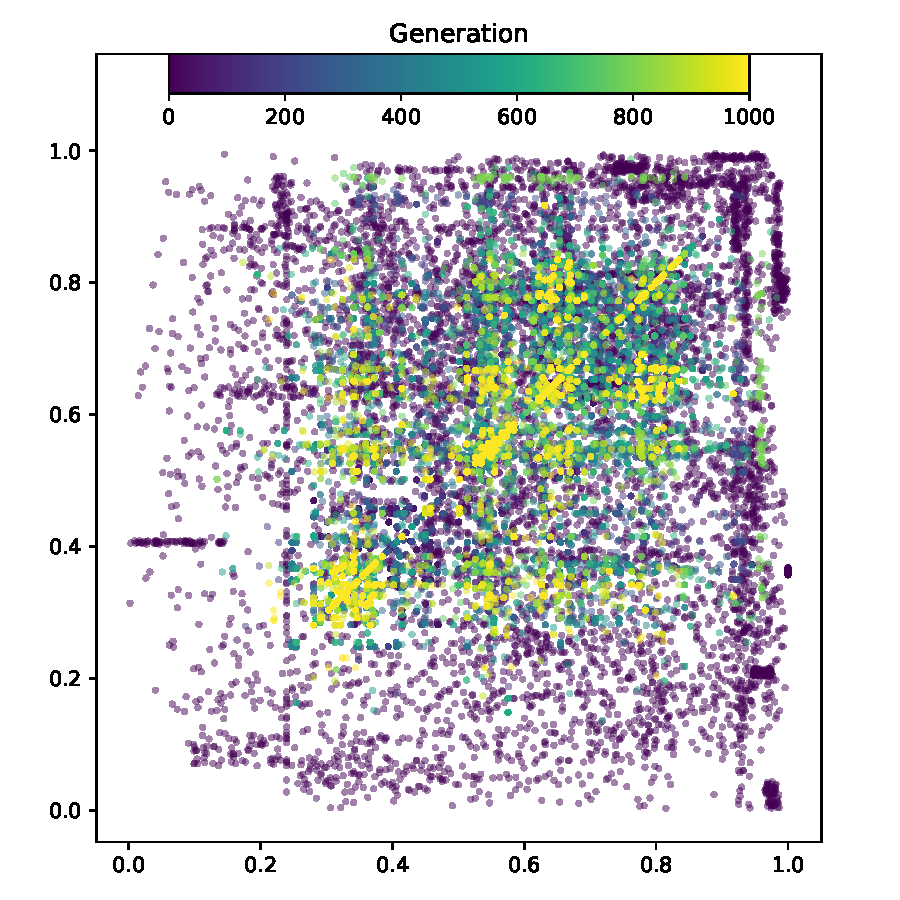
\includegraphics[width=\imgwidth]{Fig15.pdf}
    \caption{%
        A scatter of all the individuals found at 50 epoch intervals in the
        first example of Section~\ref{subsec:dbscan}, i.e.\ those summarised in
        Figure~\ref{fig:dbscan-inds}.
    }\label{fig:coverage}
\end{figure}

Although this does provide evidence to say that the current design of the EA can
sufficiently explore its given search space, it does not provide any guarantee
that this will happen, even in expectation. Proving this theoretically is an
area for further investigation.

Something that does stand against EAs is their tendency to find the `easy' way
out. That is, reducing down to the simplest solution which solves the given
problem. In most cases, that is not a problem and is often, in fact, favourable.
Throughout the case study provided, this is seen to happen.
Figure~\ref{fig:coverage} shows this behaviour again by the strong diagonal
region in later generations. In that particular example, the easiest solution
for the EA (i.e.\ for \(k\)-means to outperform DBSCAN) was to collapse one
dimension of the search space to make the problem one-dimensional. This kind of
behaviour is not necessarily a bad thing as trivial, basic and simple cases are
of great importance when understanding an algorithm's quality.

However, should that be a problem, then the objective function could be adjusted
accordingly. In the case study, several iterations of fitness functions were
examined but each was adjusted by hand according to what was apparent at the
time. Due to the architecture of the implementation of this method, this could
be done in practicality. For instance, a similar strategy could be employed
automatically by a more sophisticated fitness function that retains some
information about the datasets generated from previous runs of EDO on a
particular (or at least similar) parameter set. In this way, the currently
completely unsupervised learning conducted by the EA could be ushered away from
less helpful solutions (via some penalty, say) and toward previously unexplored
behaviours. This automatic, iterative application of the proposed method would
likely reveal more sophisticated insights into a particular algorithm.

In essence, the proposed method is merely a tool that demonstrates the benefit
of the flipped paradigm set out in this work. The concept of where `good'
datasets exist is not something that is well-documented in literature and the
hope of this work is that Evolutionary Dataset Optimisation acts as a starting
point for further works to come.


\section*{Appendix}

\subsection{Lloyd's algorithm}\label{app:kmeans}

\balg[H]%
\KwIn{a dataset \(X\), a number of centroids \(k\), a distance metric \(d\)}
\KwOut{a partition of \(X\) into \(k\) parts, \(Z\)}

\Begin{%
    select \(k\) initial centroids, \(z_1, \ldots, z_k \in X\)\;
    \While{any point changes cluster or some stopping criterion is not met}{%
        assign each point, \(x \in X\), to cluster \(Z_{j^*}\) where:
        \[
            j^* = \argmin_{j = 1, \ldots, k} \left\{%
                {d\left(x, z_j\right)}^2
            \right\}
        \]\;
        recalculate all centroids by taking the intra-cluster mean:
        \[
            z_j = \frac{1}{|Z_j|} \sum_{x \in Z_j} x
        \]
    }
}
\caption{\(k\)-means (Lloyd's)}
\ealg%

\subsection{Implementation example}\label{app:code}

Below is an example of how the Python implementation was used to complete the
first example, including the definition of the fitness function.

\begin{listing}[htbp]
\begin{usagepy}
>>> import edo
>>> import numpy as np
>>> from edo.distributions import Uniform
>>> from sklearn.cluster import KMeans
>>> 
>>> def fitness(individual, max_seeds):
...     """
...     Return the lowest final inertia of k-means on the individual dataset
...     across the given number of trials with k=2.
...     """
...     inertias, labels = [], []
...     for seed in range(max_seeds):
...         km = KMeans(n_clusters=2, random_state=seed).fit(
...             individual.dataframe
...         )
...         inertias.append(km.inertia_)
...         labels.append(km.labels_)
...     best = np.argmin(inertias)
...     individual.labels = labels[best]
...     return inertias[best]
>>> 
>>> Uniform.param_limits["bounds"] = [0, 1]
>>> families = [edo.Family(Uniform)]
>>> 
>>> opt = edo.DataOptimiser(
...     fitness,
...     size=10,
...     row_limits=[10, 50],
...     col_limits=[2, 2],
...     families=families,
...     max_iter=10,
... )
>>> pop_history, fit_history = edo.run(
...     random_state=0, fitness_kwargs={"max_seeds": 5}
... )

\end{usagepy}
\caption{Source code to produce a trial from Example~\ref{ex:edo-1}}
\end{listing}

\chapter{A game-theoretic initialisation for the \(k\)-modes algorithm}%
\label{chp:kmodes}

\graphicspath{{chapters/kmodes/paper/img/}}
\renewcommand{\algpath}{chapters/kmodes/paper/tex/algorithms}
\renewcommand{\texpath}{chapters/kmodes/paper/tex}

\begin{center}
    The research reported in this chapter has led to a manuscript
    entitled:\\[1em]

    {%
        \bf\itshape{``A novel initialisation based on hospital-resident
                    assignment for the \(k\)-modes algorithm''}
    }

    Available online at: \arxiv{2002.02701}\\

    Associated data: \doi{10.5281/zenodo.3638035}\\
    Source code: \doi{10.5281/zenodo.3639282}\\[1em]

    The abstract of the manuscript is as follows:\\[1em]
\end{center}

This chapter presents a new way of selecting an initial solution for the
\(k\)-modes algorithm that allows for a notion of game theoretic fairness that
classic initialisations, namely those by Huang and Cao, do not. The method,
which utilises the Hospital-Resident Assignment Problem to find the set of
initial cluster centroids, is compared with two initialisation methods for
\(k\)-modes: the original presented in \cite{Huang1998} and the next most
popular method present in the literature~\cite{Cao2009}. In order to highlight
the merits of the proposed method two stages of analysis are presented. The
paper concludes with an analysis of these methods against the proposed and it is
demonstrated that the proposed method is able to outperform them both. The aim
of this analysis is two-fold: first, to highlight the merits of the method in a
familiar setting by clustering well-known benchmark datasets; and second, to
provide a deeper insight into how the methods perform against one another by
generating artificial datasets using the method set out in~\cite{Wilde2019}.

\myrule%

\section{Introduction}\label{sec:intro}

In addition to the method presented by Huang, the literature revealed that the
next most commonly cited initialisation was presented in~\cite{Cao2009}. This
initialisation also forms the basis of many other initialisations where a notion
of density is central. This chapter ends with an analysis of these methods
against the proposed that demonstrates that the proposed method can outperform
them both. The aim of this analysis is two-fold: first, to highlight the merits
of the method in a familiar setting by clustering well-known benchmark datasets;
and second, to provide a more in-depth insight into how the methods perform
against one another by generating artificial datasets using the Evolutionary
Dataset Optimisation method introduced in Chapter~\ref{chp:edo}.

The chapter is structured as follows:
\begin{itemize}
    \item Section~\ref{sec:intro} introduces the \(k\)-modes algorithm and its
        established initialisation methods.
    \item Section~\ref{sec:method} provides a brief overview of
        matching games and their variants before a statement of the proposed
        initialisation.
    \item Section~\ref{sec:results} presents analyses of the initialisations
        on benchmark and new, artificial datasets.
    \item Section~\ref{sec:conclusion} concludes the chapter.
\end{itemize}


\subsection{The \(k\)-modes algorithm}\label{subsec:kmodes}

The following notation will be used throughout this chapter to describe the
objects associated with clustering a categorical dataset:

\begin{itemize}
    \item Let \(\mathcal{A} := A_1 \times \cdots \times A_m\) denote the
        \emph{attribute~space}. In this chapter, only categorical attributes are
        considered, i.e.\ for each \(j = 1, \ldots, m\) it follows that \(A_j :=
        \left\{a_1^{(j)}, \ldots, a_{d_j}^{(j)}\right\}\) where \(d_j = |A_j|\)
        is the size of the \(j^{th}\) attribute.

    \item Let \(\mathcal{X} := \left\{X^{(1)}, \ldots, X^{(N)}\right\} \subset
        \mathcal{A}\) denote a \emph{dataset} where each \(X^{(i)} \in
        \mathcal{X}\) is defined as an \(m\)-tuple \(X^{(i)} := \left(x_1^{(i)},
        \ldots, x_m^{(i)}\right)\) where \(x_j^{(i)} \in A_j\) for each \(j = 1,
        \ldots, m\). The elements of \(\mathcal{X}\) are referred to as
        \emph{data points} or \emph{instances}.
    \item Let \(\mathcal{Z} := \left(Z_1, \ldots, Z_k\right)\) be a partition
        of a dataset \(\mathcal{X} \subset \mathcal A\) into \(k \in
        \mathbb{Z}^{+}\) distinct, non-empty parts. Such a partition
        \(\mathcal{Z}\) is called a \emph{clustering} of \(\mathcal{X}\).

    \item Each cluster \(Z_l\) has associated with it a
        \emph{mode} (see Definition~\ref{def:mode}) which is
        denoted by \(z^{(l)} = \left(z_1^{(l)},~\ldots,~z_m^{(l)}\right) \in
        \mathcal{A}\).  These points are also referred to as
        \emph{representative~points} or \emph{centroids}. The set of all current
        cluster modes is denoted as \(\overline Z = \left\{z^{(1)}, \ldots,
        z^{(k)}\right\}\).
\end{itemize}

Definition~\ref{def:dissim} describes a dissimilarity measure between
categorical data points.

\begin{definition}\label{def:dissim}
    Let \(\mathcal{X} \subset \mathcal A\) be a dataset and consider any
    \(X^{(a)}, X^{(b)} \in \mathcal{X}\). The dissimilarity between \(X^{(a)}\)
    and \(X^{(b)}\), denoted by \(d\left(X^{(a)}, X^{(b)}\right)\), is given by:
    \begin{equation}\label{eq:dissim}
        d\left(X^{(a)}, X^{(b)}\right) := \sum_{j=1}^{m} \delta\left(x_j^{(a)},
        x_j^{(b)}\right) \quad \text{where} \quad \delta\left(x, y\right) =
        \begin{cases}
            0, & \text{if} \ x = y \\
            1, & \text{otherwise.}
        \end{cases}
    \end{equation}
\end{definition}

With this metric, the notion of a representative point of a cluster can be
addressed. With numeric data and \(k\)-means, such a point is simply the mean of
the points within the cluster. With categorical data, however, the mode is used
as the measure for central tendency. This change follows from the concept of
dissimilarity in that the point that best represents (i.e.\ is closest to) those
in a cluster is one with the most frequent attribute values of the points in the
cluster. The following definitions and theorem formalise this and a method to
find such a point.

\begin{definition}\label{def:mode}
    Let \(\mathcal{X} \subset \mathcal{A}\) be a dataset and consider some point
    \(z = \left(z_1, \ldots, z_m\right) \in \mathcal{A}\). Then \(z\) is called
    a \emph{mode} of \(\mathcal{X}\) if it minimises the following:
    \begin{equation}\label{eq:summed-dissim}
        D\left(\mathcal{X}, z\right) = \sum_{i=1}^{N} d\left(X^{(i)}, z\right)
    \end{equation}
\end{definition}

\begin{definition}\label{def:rel-freq}
    Let \(\mathcal{X} \subset \mathcal{A}\) be a dataset. Then
    \(n\left(a_s^{(j)}\right)\) denotes the \emph{frequency} of the \(s^{th}\)
    category \(a_s^{(j)}\) of \(A_j\) in \(\mathcal{X}\), i.e.\ for each \(A_j
    \in \mathcal{A}\) and each \(s = 1, \ldots, d_j\):
    \begin{equation}
        n\left(a_s^{(j)}\right) := \abs*{%
            {\left\{X^{(i)} \in \mathcal{X}: x_j^{(i)} = a_s^{(j)}\right\}}
        }
    \end{equation}

    Furthermore, \(\frac{n\left(a_s^{(j)}\right)}{N}\) is called the
    \emph{relative~frequency} of category \(a_s^{(j)}\) in \(\mathcal{X}\).
\end{definition}

\begin{theorem}\label{thm:mode}
    Consider a dataset \(\mathcal{X} \subset \mathcal{A}\) and some \(U = (u_1,
    \ldots, u_m) \in \mathcal{A}\). Then \(D(\mathcal{X}, U)\) is minimised if
    and only if \(n\left(u_j\right) \geq n\left(a_s^{(j)}\right)\) for all
    \(s=1, \ldots, d_j\) for each \(j = 1, \ldots, m\).

    A proof of this theorem can be found in the Appendix of~\cite{Huang1998}.
\end{theorem}

Theorem~\ref{thm:mode} defines the process by which cluster modes are updated in
\(k\)-modes (see Algorithm~\ref{alg:update}), and so the final component from
the \(k\)-means paradigm to be configured is the objective (cost) function. This
function is defined in Definition~\ref{def:cost}, and following that a practical
statement of the \(k\)-modes algorithm is given in Algorithm~\ref{alg:kmodes} as
set out in~\cite{Huang1998}.

\begin{definition}\label{def:cost}
    Let \(\mathcal{Z} = \left\{Z_1, \ldots, Z_k\right\}\) be a clustering of a
    dataset \(\mathcal{X}\), and let \(\overline Z = \left\{z^{(1)},
    \ldots, z^{(k)}\right\}\) be the corresponding cluster modes. Then \(W =
    \left(w_{i, l}\right)\) is an \(N \times k\) \emph{partition~matrix} of
    \(\mathcal{X}\) such that:
    \[
        w_{i, l} = \begin{cases}
                     1, & \text{if} \ X^{(i)} \in Z_l\\
                     0, & \text{otherwise.}
                   \end{cases}
    \]

    With this, the \emph{cost~function} is defined to be the summed
    within-cluster dissimilarity:
    \begin{equation}\label{eq:cost}
        C\left(W, \overline Z\right) := \sum_{l=1}^{k} \sum_{i=1}^{N}
        \sum_{j=1}^{m} w_{i,l} \ \delta\left(x_j^{(i)}, z_j^{(l)}\right)
    \end{equation}
\end{definition}

\inputalg{kmodes}

\subsection{Initialisation processes}\label{subsec:inits}

The standard selection method to initialise \(k\)-modes is to randomly sample
\(k\) distinct points in the dataset. In all cases, the initial modes must be
points in the dataset to ensure that there are no empty clusters in the first
iteration of the algorithm. The remainder of this section describes two
well-established initialisation methods that aim to lever the structure of the
data at hand preemptively.

\subsubsection{Huang's method}\label{subsec:huang}

Among the original works by Huang, an alternative initialisation method was
presented that selects modes by distributing frequently-occurring values from
the attribute space among \(k\) potential modes~\cite{Huang1998}. The process
referred to as Huang's method is described in full in Algorithm~\ref{alg:huang}.
Huang's method considers a set of potential modes, \(\widehat Z \subset \mathcal
A\), that is then replaced by a set of real initial modes, \(\overline Z \subset
\mathcal X\). The process of selecting this set of potential modes is ambiguous
in the original paper --- as is alluded to in~\cite{Jiang2016}.  Here, as is
done in practical implementations of \(k\)-modes, this is interpreted as being
done via a weighted random sample (see Algorithm~\ref{alg:potential_modes}).

\inputalg{huang}


\subsubsection{Cao's method}\label{subsec:cao}

The second initialisation process that is widely used with \(k\)-modes is known
as Cao's method~\cite{Cao2009}. This method selects the initial modes according
to their density in the dataset whilst forcing dissimilarity between them.
Definition~\ref{def:density} formalises the concept of density and its
relationship to relative frequency. The method, described in
Algorithm~\ref{alg:cao}, is deterministic --- unlike Huang's method, which
relies on random sampling.

\begin{definition}\label{def:density}
    Consider a dataset
    \(\mathcal{X} \subset \mathcal{A} = \{A_1, \ldots, A_m\}\). Then the
    \emph{average~density} of any point \(X_i \in \mathcal{X}\) with respect to
    \(\mathcal{A}\) is defined~\cite{Cao2009} as:
    \begin{equation}\label{eq:density}
        \text{Dens}\left(X^{(i)}\right) = \frac{%
            \sum_{j=1}^m \text{Dens}_{j}\left(X^{(i)}\right)
        }{m}
        \quad \text{where} \quad
        \text{Dens}_{j}\left(X^{(i)}\right) = \frac{%
            \abs*{%
                \left\{X^{(t)} \in \mathcal{X} : x_j^{(i)} = x_j^{(t)}\right\}
            }
        }{N}
    \end{equation}

    Observe that:
    \[
        \abs*{\left\{X^{(t)} \in \mathcal{X} : x_j^{(i)} = x_j^{(t)}\right\}}%
        = n\left(x_j^{(i)}\right)%
        = \sum_{t=1}^N \left(1 - \delta\left(x_j^{(i)}, x_j^{(t)}\right)\right)
    \]

    And so, an alternative definition for~\eqref{eq:density} can be derived:
    \begin{equation}\label{eq:density-alt}
        \text{Dens}\left(X^{(i)}\right)
        = \frac{1}{mN} \sum_{j=1}^m \sum_{t=1}^N \left(%
            1 - \delta\left(x_j^{(i)}, x_j^{(t)}\right)
        \right)
        = 1 - \frac{1}{mN} D\left(\mathcal{X}, X^{(i)}\right)
    \end{equation}
\end{definition}

\inputalg{cao}


\section{Matching games and the proposed method}\label{sec:method}

Both of the initialisation methods described in Section~\ref{subsec:inits} have
a greedy component. Cao's method essentially chooses the densest point that has
not already been chosen whilst forcing some separation between the set of
initial modes. In the case of Huang's, the greediness only comes toward the end
of the method. When the set of potential modes is identified, it is replaced by
a set of instances in the dataset. Specifically, this means that in any
practical implementation of this method, the order in which a set of potential
modes is iterated over can affect the set of initial modes. Thus, there is no
guarantee of consistency.

The initialisation proposed in this chapter extends Huang's method to be
order-invariant in the final allocation --- thereby eliminating its greedy
component --- and provides a more intuitive starting point for the \(k\)-modes
algorithm by constructing and solving a matching game between the set of
potential modes and some subset of the data.

In general, matching games are defined by two sets (parties) of players in which
each player creates a preference list of at least some of the players in the
other party. The objective then is to find a `stable' mapping between the two
sets of players such that no pair of players are (rationally) unhappy with their
matching. Algorithms to `solve' --- i.e.\ find stable matchings to --- instances
of matching games are often structured to be party-oriented and aim to maximise
some form of social or party-based
optimality~\cite{%
    Erdil2017,Fuku2006,Gale1962,Iwama2016,Kwanashie2015,Manlove2002%
}.

The particular constraints of this case --- where the \(k\) potential modes must
be allocated to a nearby unique data point --- mirror those of the so-called
Hospital-Resident Assignment Problem (HR). This problem gets its name from the
real-world problem of fairly allocating medical students to hospital posts.  A
resident-optimal algorithm for solving HR was presented in~\cite{Gale1962} and
was adapted in~\cite{Roth1984} to take advantage of the structure of the game.
This adapted algorithm is given in Algorithm~\ref{alg:hospital_resident}. The
Python library discussed in Chapter~\ref{chp:matching} is used in the
implementation of the proposed method for Section~\ref{sec:results}.

The game used to model HR, its matchings, and its notion of stability are
defined in Definitions~\ref{def:game}---\ref{def:blocking}. A summary of these
definitions in the context of the proposed \(k\)-modes initialisation is given
in Table~\ref{tab:components}. Then Algorithm~\ref{alg:proposed_method} provides
a formal statement of the proposed method.

\begin{definition}\label{def:game}
    Consider two distinct sets \(R, H\) and refer to them residents and
    hospitals. Each \(h \in H\) has a capacity \(c_h \in \mathbb{N}\) associated
    with them. Each player \(r \in R\) and \(h \in H\) has associated
    with it a strict preference list of the other set's elements such that:
    \begin{itemize}
        \item Each \(r \in R\) ranks a non-empty subset of \(H\), denoted by
            \(f(r)\).
        \item Each \(h \in H\) ranks all and only those residents that have
            ranked it, i.e.\ the preference list of \(h\), denoted \(g(h)\), is
            a permutation of the set
            \(\left\{r \in R \ | \ h \in f(r)\right\}\). If no such residents
            exist, \(h\) is removed from \(H\).
    \end{itemize}

    This construction of residents, hospitals, capacities and preference lists
    is called a \emph{game} and is denoted by \((R, H)\).
\end{definition}

\begin{definition}\label{def:matching}
    Consider a game \((R, H)\). A \emph{matching} \(M\) is any mapping between
    \(R\) and \(H\). If a pair \((r, h) \in R \times H\) are matched in \(M\)
    then this relationship is denoted \(M(r) = h\) and \(r \in M^{-1}(h)\).

    A matching is only considered \emph{valid} if all of the following hold for
    all \(r \in R, h \in H\):
    \begin{itemize}
        \item If \(r\) is matched then \(M(r) \in f(r)\).
        \item If \(h\) has at least one match then \(M^{-1}(h) \subseteq g(h)\).
        \item \(h\) is not over-subscribed, i.e.\ \(\abs*{M^{-1}(h)} \leq c_h\).
    \end{itemize}

    A valid matching is considered \emph{stable} if it does not contain any
    blocking pairs.
\end{definition}

\begin{definition}\label{def:blocking}
    Consider a game \((R, H)\). Then a pair \((r, h) \in R \times H\) is said to
    \emph{block} a matching \(M\) if all of the following hold:
    \begin{itemize}
        \item There is mutual preference, i.e.\ \(r \in g(h)\) and \(h \in
            f(r)\).
        \item Either \(r\) is unmatched or they prefer \(h\) to \(M(r)\).
        \item Either \(h\) is under-subscribed or \(h\) prefers \(r\) to at
            least one resident in \(M^{-1}(h)\).
    \end{itemize}
\end{definition}

\begin{table}[htbp]
    \resizebox{\textwidth}{!}{%
    \begin{tabular}{lcr}
        \toprule%
        Object in \(k\)-modes initialisation & {} & Object in a matching game
        \\\midrule%
        Potential modes & {} & The set of residents
        \\
        Data points closest to potential modes & {} & The set of hospitals
        \\
        Similarity between a potential mode and a point & {} & Respective
        position in each other's preference lists
        \\
        The data point to replace a potential mode & {} & A pair in a matching
        \\\bottomrule
    \end{tabular}}
    \caption{A summary of the relationships between the components of the
             initialisation for \(k\)-modes and those in a matching game
             \((R, H)\).
    }\label{tab:components}
\end{table}

\inputalg{hospital_resident}

\inputalg{proposed_method}

\section{Experimental results}\label{sec:results}

To give comparative results on the quality of the initialisation processes
considered in this chapter, four well-known, categorical, labelled datasets ---
breast cancer, mushroom, nursery, and soybean (large) --- will be clustered by
the \(k\)-modes algorithm with each of the initialisation processes. These
datasets have been chosen to fall in line with the established literature.
Further, they exhibit a range of sizes and complexities. Each dataset is openly
available under the UCI Machine Learning Repository~\cite{Dua2019}, and their
characteristics are summarised in Table~\ref{tab:dataset_summary}. This analysis
excludes all incomplete instances (i.e.\ where data is missing), and the
remaining dataset characteristics are reported as `adjusted'.

\begin{table}
    \resizebox{\textwidth}{!}{\input{\texpath/dataset_summary}}
    \caption{A summary of the benchmark datasets}\label{tab:dataset_summary}
\end{table}

This analysis does not consider evaluative metrics related to classification
such as accuracy, recall or precision as is commonly done~\cite{%
    Arthur2007,Cao2009,Cao2012,Huang1998,%
    Ng2007,Olaode2014,Schaeffer2007,Sharma2015%
}. Instead, only internal measures are considered, such as the cost function
defined in~\eqref{eq:cost}. This metric is label-invariant, and its values are
comparable across the different initialisation methods. Furthermore, the cost
function captures the effect of each initialisation method on the initial and
final clustering of each dataset. An additional, and often useful, metric is the
silhouette coefficient, which measures the ratio between the intra-cluster
cohesion and inter-cluster separation of a particular clustering. Therefore, it
could reveal the effect of each initialisation method at the beginning and end
of a run of \(k\)-modes.  Unfortunately, this metric loses its intuition under
the distance measure employed here and, as such, has been omitted. The remaining
performance measures used are the number of iterations for the \(k\)-modes
algorithm to terminate and the time to terminate in seconds.

The final piece of information required in this analysis is a choice for \(k\)
for each dataset. An immediate choice is the number of classes that are present
in a dataset but this is not necessarily an appropriate choice since the classes
may not be representative of true clusters~\cite{Memoli2011}. However, this
analysis will consider this case as there may be practical reasons to limit the
value of \(k\). The other strategy for choosing \(k\) considered in this chapter
uses the knee point detection algorithm introduced in~\cite{Satopaa2011}. This
strategy was chosen over other popular methods such as the `elbow' method as its
results are definitive.

The knee point detection algorithm was employed using values of \(k\) from 2 up
to \(\lfloor\sqrt N\rfloor\) for each dataset. The number of clusters determined
by this strategy is reported in the final column of
Table~\ref{tab:dataset_summary}.


\subsection{Using knee point detection algorithm for \(k\)}\label{subsec:knee}

Tables~\ref{tab:breast_cancer_knee}---\ref{tab:soybean_knee} summarise the
results of each initialisation method on the benchmark datasets. In each case,
the number of clusters was determined using the knee point detection algorithm.
Each column shows the mean value of each metric and its standard
\input{\texpath/repetitions.tex}repetitions of the \(k\)-modes algorithm.

\begin{table}
    \centering
    \resizebox{\textwidth}{!}{%
        \input{\texpath/knee/breast_cancer_summary.tex}
    }
    \captionof{table}{%
        Summary metric results for the breast cancer dataset with \(k=8\).
    }\label{tab:breast_cancer_knee}\vspace{2em}

    \resizebox{\textwidth}{!}{%
        \input{\texpath/knee/mushroom_summary.tex}
    }
    \captionof{table}{%
        Summary metric results for the mushroom dataset with \(k=17\).
    }\label{tab:mushroom_knee}\vspace{2em}

    \resizebox{\textwidth}{!}{%
        \input{\texpath/knee/nursery_summary.tex}
    }
    \captionof{table}{%
        Summary metric results for the nursery dataset with \(k=23\).
    }\label{tab:nursery_knee}\vspace{2em}

    \resizebox{\textwidth}{!}{%
        \input{\texpath/knee/soybean_summary.tex}
    }
    \captionof{table}{%
        Summary metric results for the soybean dataset with \(k=8\).
    }\label{tab:soybean_knee}
\end{table}

By examining these tables, it would seem that the proposed method and Huang's
method are comparable across the board --- although the proposed method is
faster despite taking more iterations in general which may relate to a more
intuitive initialisation. More importantly, though, it appears that Cao's method
performs the best out of the three initialisation methods: in terms of initial
and final costs Cao's method improves, on average, by roughly 10\% against the
next best method for the three datasets that it succeeds with; the number of
iterations is comparable; the computation time is substantially less than the
other two considering it is a deterministic method and need only be run once to
achieve this performance.

However, in the \(k\)-means paradigm, a particular clustering is selected based
on it having the minimal final cost over several runs of the algorithm --- not
the mean --- and while Cao's method is very reliable, in that there is no
variation at all, it does not always produce the best clustering possible. There
is a trade-off to be made between computational time and performance here. In
order to gain more insight into the performance of each method, less granular
analysis is required.

Figures~\ref{fig:breast_cancer_knee}---\ref{fig:soybean_knee} display the cost
function results for each dataset in the form of a scatter plot and two
empirical cumulative density function (CDF) plots, highlighting the breadth and
depth of the behaviours exhibited by each initialisation method.

Looking at Figure~\ref{fig:breast_cancer_knee}, it is clear that in terms of the
final cost, Cao's method is middling when compared to the other methods. This
so-so performance is apparent from Table~\ref{tab:breast_cancer_knee} and,
indeed, Huang's and the proposed method are both very comparable when looking at
the main body of the results. However, since the criterion for the best
clustering (in practical terms) is having the minimal final cost, it is evident
that the proposed method is superior; that the method produces clusterings with
a broader range of costs (indicated by the trailing right-hand side of each CDF
plot) is irrelevant for the same reason.

This pattern of broadly similar behaviour between Huang's and the proposed
method is apparent in each of the figures here, and in each case, the proposed
method outperforms Huang's. In fact, for all cases except for the nursery
dataset, the proposed method achieves the lowest final cost of all the methods.
As such, it performs the best in practical terms on these particular datasets.

In the case of the nursery dataset, Cao's method is unquestionably the best
performing initialisation method. It should be noted that none of the methods
was able to find an initial clustering that could be improved on, and that this
dataset exactly describes the entire attribute space in which it exists. This
property could be why the other methods fall behind Cao's method so decisively
in that it can definitively choose the \(k\) most dense-whilst-separated points
from the attribute space as the initial cluster centres whereas the other two
methods are in essence randomly sampling from this space. That each initial
solution in these repetitions is locally optimal remains a mystery.

\begin{figure}
    \begin{subfigure}{.5\textwidth}
        \includegraphics[width=\linewidth]{Fig1a.pdf}
        \caption{Scatter plot of initial and final costs.}
    \end{subfigure}
    \hfill%
    \begin{subfigure}{.5\textwidth}
        \includegraphics[width=\linewidth]{Fig1b1.pdf}

        \includegraphics[width=\linewidth]{Fig1b2.pdf}
        \caption{Empirical CDF plots for initial (top) and final (bottom)
                 costs.}
    \end{subfigure}
    \caption{Summary plots for the breast cancer dataset with \(k=8\).}%
    \label{fig:breast_cancer_knee}
\end{figure}

\begin{figure}
    \begin{subfigure}{.5\textwidth}
        \includegraphics[width=\linewidth]{Fig2a.pdf}
        \caption{Scatter plot of initial and final costs.}
    \end{subfigure}
    \hfill%
    \begin{subfigure}{.5\textwidth}
        \includegraphics[width=\linewidth]{Fig2b1.pdf}

        \includegraphics[width=\linewidth]{Fig2b2.pdf}
        \caption{Empirical CDF plots for initial (top) and final (bottom)
                 costs.}
    \end{subfigure}
    \caption{Summary plots for the mushroom dataset with \(k=17\).}%
    \label{fig:mushroom_knee}
\end{figure}

\begin{figure}
    \begin{subfigure}{.5\textwidth}
        \includegraphics[width=\linewidth]{Fig3a.pdf}
        \caption{Scatter plot of initial and final costs.}
    \end{subfigure}
    \hfill%
    \begin{subfigure}{.5\textwidth}
        \includegraphics[width=\linewidth]{Fig3b1.pdf}

        \includegraphics[width=\linewidth]{Fig3b2.pdf}
        \caption{Empirical CDF plots for initial (top) and final (bottom)
                 costs.}
    \end{subfigure}
    \caption{Summary plots for the nursery dataset with \(k=23\).}%
    \label{fig:nursery_knee}
\end{figure}

\begin{figure}
    \begin{subfigure}{.5\textwidth}
        \includegraphics[width=\linewidth]{Fig4a.pdf}
        \caption{Scatter plot of initial and final costs.}
    \end{subfigure}
    \hfill%
    \begin{subfigure}{.5\textwidth}
        \includegraphics[width=\linewidth]{Fig4b1.pdf}

        \includegraphics[width=\linewidth]{Fig4b2.pdf}
        \caption{Empirical CDF plots for initial (top) and final (bottom)
                 costs.}
    \end{subfigure}
    \caption{Summary plots for the soybean dataset with \(k=8\).}%
    \label{fig:soybean_knee}
\end{figure}


\subsection{Using number of classes for \(k\)}\label{subsec:nclasses}

As is discussed above, the often automatic choice for \(k\) is the number of
classes present in the data. This subsection repeats the analysis from the
previous subsection but with this traditional choice for \(k\).
Tables~\ref{tab:breast_cancer_nclasses}---\ref{tab:soybean_nclasses} contain the
analogous summaries of each initialisation method's performance on the benchmark
datasets over the same number of repetitions.

\begin{table}[htbp]
    \centering
    \resizebox{\textwidth}{!}{%
        \input{\texpath/nclasses/breast_cancer_summary.tex}
    }
    \captionof{table}{%
        Summary metric results for the breast cancer dataset with \(k=2\).
    }\label{tab:breast_cancer_nclasses}\vspace{2em}

    \resizebox{\textwidth}{!}{%
        \input{\texpath/nclasses/mushroom_summary.tex}
    }
    \captionof{table}{%
        Summary metric results for the mushroom dataset with \(k=2\).
    }\label{tab:mushroom_nclasses}\vspace{2em}

    \resizebox{\textwidth}{!}{%
        \input{\texpath/nclasses/nursery_summary.tex}
    }
    \captionof{table}{%
        Summary metric results for the nursery dataset with \(k=5\).
    }\label{tab:nursery_nclasses}\vspace{2em}

    \resizebox{\textwidth}{!}{%
        \input{\texpath/nclasses/soybean_summary.tex}
    }
    \captionof{table}{%
        Summary metric results for the soybean dataset with \(k=15\).
    }\label{tab:soybean_nclasses}
\end{table}

An immediate comparison to the previous tables is that the mean costs are
significantly higher, and the computation times are shorter, for all datasets
bar the soybean dataset. These effects come directly from the choice of \(k\) in
that higher values of \(k\) will require more checks (and thus computational
time) but will typically lead to more homogeneous clusters, reducing their
within-cluster dissimilarity and therefore cost.

Looking at these tables on their own reveals that Cao's method is the superior
initialisation method on average: the means are substantially lower in terms of
initial and final cost; there is no deviation in these results; again, the total
computational time is a fraction of the other two methods. It is also apparent
that Huang's method and the proposed extension are very comparable on average.
As before, a more nuanced investigation will require finer visualisations.

Figures~\ref{fig:breast_cancer_nclasses}---\ref{fig:soybean_nclasses} show the
analogous plots as in the previous subsection except with this traditional
choice for \(k\).

Figures~\ref{fig:breast_cancer_nclasses}~\&~\ref{fig:mushroom_nclasses} indicate
that a particular behaviour emerged during the runs of the \(k\)-modes
algorithm. Specifically, each solution falls into one of (predominantly) two
types: effectively no improvement on the initial clustering, or terminating at
some clustering with a cost that is bounded below across all such solutions.
Invariably, Cao's method achieves or approaches this lower bound, and unless
Cao's method is used, these particular choices for \(k\) mean that the
performance of the \(k\)-modes algorithm is susceptible to its initial
clustering. Moreover, the other two methods are effectively indistinguishable in
these cases, and so if a robust solution is required, Cao's method is the only
viable option.

Figure~\ref{fig:nursery_nclasses} corresponds to the nursery dataset results
with \(k=5\). In this set of runs, the same pattern emerges as in
Figure~\ref{fig:nursery_knee} where sampling the initial centres from amongst
the densest points (via Huang's method and the proposed) is an inferior strategy
to one considering the entire attribute space such as with Cao's method. Again,
no method can improve on the initial solution except for one repetition with the
matching initialisation method.

\begin{figure}
    \begin{subfigure}{.5\textwidth}
        \includegraphics[width=\linewidth]{Fig5a.pdf}
        \caption{Scatter plot of initial and final costs.}
    \end{subfigure}
    \hfill%
    \begin{subfigure}{.5\textwidth}
        \includegraphics[width=\linewidth]{Fig5b1.pdf}

        \includegraphics[width=\linewidth]{Fig5b2.pdf}
        \caption{Empirical CDF plots for initial (top) and final (bottom)
                 costs.}
    \end{subfigure}
    \caption{Summary plots for the breast cancer dataset with \(k=2\).}%
    \label{fig:breast_cancer_nclasses}
\end{figure}

\begin{figure}
    \begin{subfigure}{.5\textwidth}
        \includegraphics[width=\linewidth]{Fig6a.pdf}
        \caption{Scatter plot of initial and final costs.}
    \end{subfigure}
    \hfill%
    \begin{subfigure}{.5\textwidth}
        \includegraphics[width=\linewidth]{Fig6b1.pdf}

        \includegraphics[width=\linewidth]{Fig6b2.pdf}
        \caption{Empirical CDF plots for initial (top) and final (bottom)
                 costs.}
    \end{subfigure}
    \caption{Summary plots for the mushroom dataset with \(k=2\).}%
    \label{fig:mushroom_nclasses}
\end{figure}

\begin{figure}
    \begin{subfigure}{.5\textwidth}
        \includegraphics[width=\linewidth]{Fig7a.pdf}
        \caption{Scatter plot of initial and final costs.}
    \end{subfigure}
    \hfill%
    \begin{subfigure}{.5\textwidth}
        \includegraphics[width=\linewidth]{Fig7b1.pdf}

        \includegraphics[width=\linewidth]{Fig7b2.pdf}
        \caption{Empirical CDF plots for initial (top) and final (bottom)
                 costs.}
    \end{subfigure}
    \caption{Summary plots for the nursery dataset with \(k=5\).}%
    \label{fig:nursery_nclasses}
\end{figure}

\begin{figure}
    \begin{subfigure}{.5\textwidth}
        \includegraphics[width=\linewidth]{Fig8a.pdf}
        \caption{Scatter plot of initial and final costs.}
    \end{subfigure}
    \hfill%
    \begin{subfigure}{.5\textwidth}
        \includegraphics[width=\linewidth]{Fig8b1.pdf}

        \includegraphics[width=\linewidth]{Fig8b2.pdf}
        \caption{Empirical CDF plots for initial (top) and final (bottom)
                 costs.}
    \end{subfigure}
    \caption{Summary plots for the soybean dataset with \(k=15\).}%
    \label{fig:soybean_nclasses}
\end{figure}

The primary conclusion from this analysis is that while Huang's method is mostly
comparable to the proposed extension, there is no substantial evidence from
these use cases to use Huang's method over the one proposed in this chapter.
Figure~\ref{fig:soybean_nclasses} is the only instance where Huang's method was
able to outperform the proposed method. Other than this, the proposed method
consistently performs better (or as well as) Huang's method in terms of minimal
final costs and computational time. This success occurs when an external
framework is imposed on the data (by choosing \(k\) to be the number of classes)
and not. Furthermore, though not discussed here, the matching initialisation
method has the scope to allow for expert or prior knowledge to be included in an
initial clustering by using some ad hoc preference list mechanism.

\subsection{Artificial datasets}\label{subsec:artificial}

All of the results leading up to this point were created using benchmark
datasets, and while there are certainly benefits to comparing methods in this
way, it does not afford a rich understanding of how any of them perform more
generally. This stage of the analysis relies on a method for generating
artificial datasets introduced in~\cite{Wilde2019}. In essence, this method is
an evolutionary algorithm which acts on entire datasets to explore the space in
which potentially all possible datasets exist. The critical component of this
method is an objective function that takes a dataset and returns a value that is
to be minimised; this function is referred to as the fitness function.

In order to reveal the nuances in the performance of Cao's method and the
proposed initialisation on a particular dataset, two cases are considered: where
Cao's method outperforms the proposed, and vice versa. Both cases use the same
fitness function --- with the latter using its negative --- which is defined as
follows:
\begin{equation}\label{eq:fitness}
    f\left(\mathcal X\right) = C_{\mathrm{cao}} - C_{\mathrm{match}}
\end{equation}

Here, \(C_{\mathrm{cao}}\) and \(C_{\mathrm{match}}\) are the final costs when a
dataset \(\mathcal X\) is clustered using Cao's method and the proposed matching
method respectively with \(k = 3\). For the sake of computational time, the
proposed initialisation was given 25 repetitions. Apart from the sign of \(f\),
the dataset generation processes used identical parameters in each case and the
datasets considered here are all of a similar shape.

\begin{figure}
    \centering
    \includegraphics[width=\imgwidth]{Fig9.pdf}
    \caption{%
        Histograms of fitness for the top performing percentile in each case.
    }\label{fig:fitness}
\end{figure}

This process yielded approximately 35,000 unique datasets for each case, and the
subsequent analysis only considers the top-performing percentile of datasets
from each. Figure~\ref{fig:fitness} shows the fitness distribution of the top
percentile in each case. It should be clear from~\eqref{eq:fitness} that large
negative values are preferable here. With that, and bearing in mind that the
generation of these datasets was parameterised consistently, it appears that the
attempt to outperform Cao's method proved somewhat more straightforward, as is
indicated by the substantial difference in the locations of the fitness
distributions.

Given the quantity of data available, to understand the patterns that have
emerged, they must be summarised; in this case, univariate statistics are used.
Despite the datasets all being of similar shapes, there are some discrepancies.
With the number of rows, this is less of an issue, but any comparison of
statistics across datasets of different widths is difficult without prior
knowledge of the datasets. Moreover, there is no guarantee of contingency
amongst the attributes, and the comparison of more than a handful of variables
becomes complicated even when the attributes are identifiable. To combat this
and bring uniformity to the datasets each dataset is represented as their first
principal component obtained via centred Principal Component Analysis
(PCA)~\cite{Jolliffe1986}. While some subtleties may be lost, this
representation captures the essential characteristics of each dataset in a
single variable meaning they can be compared directly.

Since the transformation by PCA is centred, all measures for central tendency
are moot. The mean and median are not interpretable here, given that the
original data is categorical. As such, the univariate statistics used here
describe the spread and shape of the principal components and are split into two
groups:
\begin{itemize}
    \item Central moments: variance, skewness and kurtosis.
    \item Empirical quantiles: interquartile range, lower decile and upper
        decile.
\end{itemize}

Figures~\ref{fig:edo_moments}~\&~\ref{fig:edo_quantiles} show the distributions
of the six univariate statistics across all of the principal components in each
case. In addition to this, they show a fitted Gaussian kernel density
estimate~\cite{Bashtannyk2001} to accentuate the general shape of the
histograms. What becomes immediately clear from each of these plots is that for
datasets where Cao's method succeeds, the general spread of their first
principal component is much tighter than in the case where the proposed
initialisation method succeeds. This observation is particularly evident in
Figure~\ref{fig:edo_variance} where relatively low variance in the first case
indicates a higher level of density in the original categorical data.

The quantiles echo this same observation. Although Figure~\ref{fig:edo_iqr}
suggests that the components of Cao-preferable datasets can have higher
interquartile ranges than in the second case, the lower and upper deciles tend
to be closer together as is seen in
Figures~\ref{fig:edo_lower}~\&~\ref{fig:edo_upper}, suggesting that despite the
body of the component is spread, its extremities are not.

In Figures~\ref{fig:edo_skewness}~\&~\ref{fig:edo_kurtosis}, the most notable
contrast between the two cases is the range in values for both skewness and
kurtosis, which supports the evidence thus far that individual datasets have
higher densities and lower variety (i.e.\ tighter extremities) when Cao's method
succeeds over the proposed initialisation. In particular, larger values of
skewness and kurtosis translate to a high level of similarity between the
instances in a categorical dataset which is equivalent to having high density.

Overall, this analysis has revealed that if a dataset shows clear evidence of
high-density points, then Cao's method should be used over the proposed method.
However, if there is no such evidence, the proposed method can find a
substantially better clustering than Cao's method.

\begin{figure}
    \centering
    \begin{subfigure}{\imgwidth}
        \includegraphics[width=\linewidth]{Fig10a.pdf}%
        \caption{}\label{fig:edo_variance}
    \end{subfigure}

    \begin{subfigure}{\imgwidth}
        \includegraphics[width=\linewidth]{Fig10b.pdf}%
    \caption{}\label{fig:edo_skewness}
    \end{subfigure}

    \begin{subfigure}{\imgwidth}
        \includegraphics[width=\linewidth]{Fig10c.pdf}%
        \caption{}\label{fig:edo_kurtosis}
    \end{subfigure}
    \caption{Distribution plots for the (\subref{fig:edo_variance}) variance,
        (\subref{fig:edo_skewness}) skewness and (\subref{fig:edo_kurtosis})
        kurtosis of the first principal components in each
        case.}\label{fig:edo_moments}
\end{figure}

\begin{figure}
    \centering
    \begin{subfigure}{\imgwidth}
        \includegraphics[width=\linewidth]{Fig11a.pdf}
        \caption{}\label{fig:edo_iqr}
    \end{subfigure}\vfill%

    \begin{subfigure}{\imgwidth}
        \includegraphics[width=\linewidth]{Fig11b.pdf}
        \caption{}\label{fig:edo_lower}
    \end{subfigure}\vfill%

    \begin{subfigure}{\imgwidth}
        \includegraphics[width=\linewidth]{Fig11c.pdf}
        \caption{}\label{fig:edo_upper}
    \end{subfigure}
    \caption{Distribution plots for the (\subref{fig:edo_iqr}) interquartile
        range, (\subref{fig:edo_lower}) lower decile and
        (\subref{fig:edo_upper}) upper decile of the first principal components
        in each case.}\label{fig:edo_quantiles}
\end{figure}



\section{Chapter summary}\label{sec:summary}

This chapter has introduced a novel initialisation method for the \(k\)-modes
algorithm that builds on the method set out in the seminal
paper~\cite{Huang1998}; the new method models the final `replacement' process in
the original as an instance of the Hospital-Resident Assignment Problem that may
be solved to be mathematically fair and stable.

Following a thorough description of the \(k\)-modes algorithm and the
established initialisation methods, a comparative analysis was conducted amongst
the three initialisations using both benchmark and artificial datasets. This
analysis revealed that the proposed initialisation was able to outperform both
of the other methods when the choice of \(k\) was optimised according to a
mathematically rigorous elbow method. However, the proposed method was unable to
beat Cao's method (established in~\cite{Cao2009}) when an external framework was
imposed on each dataset by choosing \(k\) to be the number of classes present.

The proposed method should be employed over Cao's when there are no rigid
restrictions on what \(k\) may be, or if there is no direct evidence that the
dataset at hand has some notion of high density. Otherwise, Cao's method remains
the most reliable initialisation in terms of computational time and final cost.

\chapter{Segmentation and the recovery of queuing parameters}

\graphicspath{{chapters/copd/paper/img/}}
\renewcommand{\texpath}{chapters/copd/paper/tex}

\begin{center}
    The research reported in this chapter has led to a manuscript
    entitled:\\[1em]

    {%
        \bf\itshape{``Segmentation analysis and the recovery of queuing
                    parameters via the Wasserstein distance: a study of
                    administrative data for patients with chronic obstructive
                    pulmonary disease''}
    }

    Available online at: \arxiv{2008.04295}\\
    Associated data: \doi{10.5281/zenodo.3924715}\\
    Source code: \doi{10.5281/zenodo.3936479}\\[2em]

    The abstract of the manuscript is as follows:\\[1em]
\end{center}

This work uses a data-driven approach to analyse how the resource requirements
of patients with chronic obstructive pulmonary disease (COPD) may change,
quantifying how those changes impact the hospital system with which the patients
interact. This approach is composed of a novel combination of often distinct
modes of analysis: segmentation, operational queuing theory, and the recovery of
parameters from incomplete data. By combining these methods as presented here,
this work demonstrates that potential limitations around the availability of
fine-grained data can be overcome. Thus, finding useful operational results
despite using only administrative data.

The paper begins by finding a useful clustering of the population from this
granular data that feeds into a multi-class \(M/M/c\) model, whose parameters
are recovered from the data via parameterisation and the Wasserstein distance.
This model is then used to conduct an informative analysis of the underlying
queuing system and the needs of the population under study through several
what-if scenarios.

The analyses used to form and study this model consider, in effect, all types of
patient arrivals and how those types impact the system. With that, this study
finds that there are no quick solutions to reduce the impact of COPD patients on
the system, including adding capacity to the system. In this analysis, the only
effective intervention to reduce the strain caused by those presenting with COPD
is to enact external policies which directly improve the overall health of the
COPD population before they arrive at the hospital.

\myrule%

\section{Introduction}\label{sec:intro}

Population health research is increasingly based on data-driven methods (as
opposed to those designed solely by clinical experts) for patient-centred care
through the advent of accessible software and a relative abundance of electronic
data. However, many such methods rely heavily on detailed data — about both the
healthcare system and its population — which may limit research where
sophisticated data pipelines are not yet in place.

This work demonstrates a method of overcoming this, using routinely gathered,
administrative hospital data to build a clustering that feeds into a multi-class
queuing model, allowing for better understanding of the healthcare population
and the system with which they interact. Specifically, this work examines
records of patient spells from the National Health Service (NHS) Wales Cwm Taf
Morgannwg University Health Board (UHB) presenting chronic obstructive pulmonary
disease (COPD). COPD is a condition of particular interest to population health
research, and to Cwm Taf Morgannwg UHB, as it is known to often present as a
comorbidity in patients~\cite{Houben2019}, increasing the complexity of
treatments among those with the condition. Moreover, an internal report by NHS
Wales found the Cwm Taf Morgannwg UHB had the highest prevalence of the
condition across all the Welsh health boards.

This work draws upon several overlapping sources within mathematical research,
and this work contributes to the literature in three ways: to theoretical
queuing research by the estimation of missing queuing parameters with the
Wasserstein distance; to operational healthcare research through the weaving
together of the combination of methods used in this work despite data
constraints; and to public health research by adding to the growing body of
mathematical and operational work around a condition that is vital to understand
operationally, socially and medically.

The remainder of the paper is structured as follows: Section~\ref{sec:intro}
provides a literature review, and an overview of the dataset and its clustering;
Section~\ref{sec:model} describes the queuing model used and the estimation of
its parameters; Section~\ref{sec:scenarios} presents several what-if scenarios
with insight provided by the model parameterisation and the clustering;
Section~\ref{sec:conclusion} concludes the paper. Although the data is
confidential and may not be published, a synthetic analogue has been
archived~\cite{Wilde2020synthetic} along with all the source code used in this
paper~\cite{Wilde2020github}.


\subsection{Literature review}\label{subsec:review}

Given the subject matter of this work, the relevant literature spans much of
operational research in healthcare, and the focus of this review is on the
critical topics of segmentation analysis, queuing models applied to hospital
systems, and the handling of missing or incomplete data for such queues.

\subsubsection{Segmentation analysis}

Segmentation analysis allows for the targeted analysis of otherwise
heterogeneous datasets and encompasses several techniques from operational
research, statistics and machine learning. One of the most desirable qualities
of this kind of analysis is the ability to glean and communicate simplified
summaries of patient needs to stakeholders within a healthcare
system~\cite{Vuik2016b, Yoon2020}. For instance, clinical profiling often forms
part of the broader analysis where each segment is summarised in a phrase or
infographic~\cite{Vuik2016a, Yan2019}.

The review for this work identified three commonplace groups of patient
characteristics used to segment a patient population: system utilisation
metrics; clinical attributes; and the pathway. The last is not used to segment
the patients directly, instead of grouping their movements through a healthcare
system, typically via process mining.~\cite{Arnolds2018}~and~\cite{Delias2015}
demonstrate how this technique can be used to improve the efficiency of a
hospital system as opposed to tackling the more relevant issue of
patient-centred care. The remaining characteristics can be segmented in a
variety of ways, but recent works tend to favour unsupervised methods —
typically latent class analysis (LCA) or clustering~\cite{Yan2018}.

LCA is a statistical, model-based method used to identify groups (called latent
classes) in data by relating its observations to some unobserved (latent),
categorical attribute. This attribute has multiple possible categories, each
corresponding to a latent class. The discovered relations enable the
observations to be separated into latent classes according to their maximum
likelihood class membership~\cite{Hagenaars2002,Lazarsfeld1968}. This method has
proved useful in the study of comorbidity patterns as
in~\cite{Kuwornu2014,Larsen2017} where combinations of demographic and clinical
attributes are related to various subgroups of chronic diseases.

Similarly to LCA, clustering identifies groups (clusters) in data to produce
labels for its instances. However, clustering includes a wide variety of methods
where the common theme is to maximise homogeneity within, and heterogeneity
between, each cluster~\cite{Everitt2011}. The \(k\)-means paradigm is the most
popular form of clustering in literature. The method iteratively partitions
numerical data into \(k \in \mathbb N\) distinct parts where \(k\) is fixed a
priori. This method has proved popular as it is easily scalable, and its
implementations are concise~\cite{Olafsson2008,Wu2009}. In addition to
\(k\)-means, hierarchical clustering methods can be useful if a suitable number
of parts cannot be found initially~\cite{Vuik2016a}. However, supervised
hierarchical segmentation methods such as classification and regression trees
(as in~\cite{Harper2006}) have been used where an existing, well-defined, label
is of particular significance.

\subsubsection{Queuing models}

Since the seminal works by Erlang~\cite{Erlang1917,Erlang1920} established the
core concepts of queuing theory, the application of queues and queuing networks
to real services has become abundant, including the healthcare service. By
applying these models to healthcare settings, many aspects of the underlying
system can be studied. A common area of study in healthcare settings is of
service capacity.~\cite{McClain1976} is an early example of such work where
acute bed capacity was determined using hospital occupancy data. Meanwhile, more
modern works such as~\cite{Palvannan2012,Pinto2014} consider more extensive
sources of data to build their queuing models.  Moreover, the output of a model
is catered more towards being actionable --- as is the prerogative of
operational research. For instance,~\cite{Pinto2014} devises new categorisations
for both hospital beds and arrivals that are informed by the queuing model. A
further example is~\cite{Komashie2015} where queuing models are used to measure
and understand satisfaction among patients and staff.

In addition to these theoretic models, healthcare queuing research has expanded
to include computer simulation models. The simulation of queues, or networks
thereof, have the benefit of adeptly capturing the stochastic nuances of
hospital systems over their theoretic counterparts. Example areas include the
construction and simulation of Markov processes via process
mining~\cite{Arnolds2018,Rebuge2012}, and patient flow~\cite{Bhattacharjee2014}.
Regardless of the advantages of simulation models, a prerequisite is reliable
software with which to construct those simulations. A common approach to
building simulation models of queues is to use a graphical user interface such
as Simul8. These tools have the benefits of being highly visual, making them
attractive to organisations looking to implement queuing models without
necessary technical expertise, including the NHS.~\cite{Brailsford2013}
discusses the issues around operational research and simulation being taken up
in the NHS despite the availability of intuitive software packages like Simul8.
However, they do not address a core principle of good simulation work:
reproducibility. The ability to reliably reproduce a set of results is of great
importance to scientific research but remains an issue in simulation research
generally~\cite{Fitzpatrick2019}. When considering issues with reproducibility
in scientific computing (simulation included), the source of any concerns is
often with the software used~\cite{Ivie2018}. Using well-developed, open-source
software can alleviate issues around reproducibility and reliability as how they
are used involve less uncertainty and require more rigour than ‘drag-and-drop’
software. One example of such a piece of software is Ciw~\cite{Palmer2019}. Ciw
is a discrete event simulation library written in Python that is fully
documented and tested. The simulations constructed and studied in
Sections~\ref{sec:model}~and~\ref{sec:scenarios} utilise this library and aid
the overall reproducibility of this work.

\subsubsection{Handling incomplete queue data}

As is discussed in other parts of this section, the data available in this work
is not as detailed as in other comparative works. Without access to such data
--- but intending to gain insight from what is available --- it is
imperative to bridge the gap left by the incomplete data.

Moreover, it is often the case that in practical situations where suitable data
is not (immediately) available, further inquiry in that line of research will
stop. Queuing models in healthcare settings appear to be such a case; the line
ends at incomplete queue data.~\cite{Asanjarani2017} is a bibliographic work
that collates articles on the estimation of queuing system characteristics ---
including their parameters. Despite its breadth of almost 300 publications from
1955, only two articles have been identified as being applied to
healthcare:~\cite{Mohammadi2012,Yom2014}. Both works are concerned with
customers who can re-enter services during their time in the queuing system,
which is mainly of value when considering the effect of unpredictable behaviour
in intensive care units, for instance.~\cite{Mohammadi2012} seeks to approximate
service and re-service densities through a Bayesian approach and by filtering
out those customers seeking to be serviced again. On the other
hand,~\cite{Yom2014} considers an extension to the \(M/M/c\) queue with direct
re-entries. The devised model is then used to determine resource requirements in
two healthcare settings.

Aside from healthcare-specific works, the approximation of queue parameters has
formed a part of relevant modern queuing research. However, the scope is
primarily focused on theoretic approximations rather than by
simulation.~\cite{Djabali2018,Goldenshluger2016} are two such recent works that
consider an underlying process to estimate a general service time distribution
in single server and infinite server queues respectively.

\subsection{Overview of the dataset and its clustering}\label{subsec:overview}

The Cwm Taf Morgannwg UHB provided the dataset used in this work. The
dataset contains an administrative summary of 5,231 patients presenting COPD
from February 2011 through March 2019 totalling 10,861 spells. A patient
(hospital) spell is defined as the continuous stay of a patient using a hospital
bed on premises controlled by a healthcare provider and is made up of one or
more patient episodes~\cite{NHS2020}. The following attributes describe the
spells included in the dataset:
\begin{itemize}
    \item Personal identifiers and information, i.e.\ patient and spell ID
        numbers, and identified gender;
    \item Admission/discharge dates and approximate times;
    \item Attributes summarising the clinical path of the spell including
        admission/discharge methods, and the number of episodes, consultants and
        wards in the spell;
    \item International Classification of Diseases (ICD) codes and primary
        Healthcare Resource Group (HRG) codes from each episode;
    \item Indicators for any COPD intervention. The value for any given instance
        in the dataset (i.e. a spell) is one of no intervention, pulmonary
        rehabilitation (PR), specialist nursing (SN), and both interventions;
    \item Charlson Comorbidity Index (CCI) contributions from several long term
        conditions (LTCs) as well as indicators for some other conditions such
        as sepsis and obesity. CCI is useful in anticipating hospital
        utilisation as a measure for the burdens associated with
        comorbidity~\cite{Simon2011};
    \item Rank under the 2019 Welsh Index of Multiple Deprivation (WIMD),
        indicating relative deprivation of the postcode area the patient lives
        in which is known to be linked to COPD prevalence and
        severity~\cite{Collins2018,Sexton2016,Steiner2017}.
\end{itemize}

In addition to the above, the following attributes were engineered for each
spell:
\begin{itemize}
    \item Age and spell cost data were linked to approximately half of the
        spells in the dataset from another administrative dataset provided by
        the Cwm Taf Morgannwg UHB;
    \item The presenting ICD codes were generalised to their categories
        according to NHS documentation and counts for each category were
        attached. This reduced the number of values from
        1,926 codes to 21 categories;
    \item A measure of admission frequency was calculated by taking the number
        of COPD-related admissions in the last twelve months linked to the
        associated patient ID number.
\end{itemize}

Although there is a fair amount of information here, it is limited to
COPD-related admissions. Therefore, rather than segmenting the patients
themselves, the spells will be. The clustering algorithm of choice is a variant
of \(k\)-means, called \(k\)-prototypes, allows for the clustering of mixed-type
data by performing \(k\)- means on the numeric attributes and \(k\)-modes on the
categorical. Both \(k\)-prototypes and \(k\)-modes were presented
in~\cite{Huang1998}.

The attributes included in the clustering encompass both utilisation metrics and
clinical attributes relating to the spell. They comprise the summary clinical
path attributes, the CCI contributions and condition indicators, the WIMD rank,
length of stay (LOS), COPD intervention status, and the engineered attributes
(not including age and costs due to lack of coverage).

To determine the optimal number of clusters, \(k\), the knee point detection
algorithm introduced in~\cite{Satopaa2011} was used with a range of potential
values for \(k\) from two to 10. This range was chosen based on what may be
considered feasibly informative to stakeholders. The knee point detection
algorithm can be considered a deterministic version of the widely known `elbow
method' for determining the number of clusters. Applying this algorithm
revealed an optimal value for \(k\) of four, but both three and five clusters
were considered. Both of these cases were eliminated due to a lack of clear
separation in the characteristics of the clusters. Additionally, the
initialisation method used for \(k\)-prototypes was presented
in~\cite{Wilde2020} as it was found to give an improvement in the clustering
over other initialisation methods.

\begin{table}
    \centering
    \resizebox{\tabwidth}{!}{%
        \begin{tabular}{llrrrrr}
\toprule
               &        &  Cluster &          &          &           & Population \\
               &        &        0 &        1 &        2 &         3 &            \\
\midrule
\textbf{Characteristics} & \textbf{Percentage of spells} &     9.91 &    19.27 &    69.39 &      1.44 &     100.00 \\
               & \textbf{Mean spell cost, £} &  8051.23 &  2309.63 &  1508.41 &  17888.43 &    2265.40 \\
               & \textbf{Percentage of recorded costs} &    29.01 &    19.38 &    48.20 &      3.40 &     100.00 \\
               & \textbf{Median age} &    77.00 &    77.00 &    71.00 &     82.00 &      73.00 \\
               & \textbf{Minimum LOS} &    12.82 &    -0.00 &    -0.02 &     48.82 &      -0.02 \\
               & \textbf{Mean LOS} &    25.30 &     6.46 &     4.11 &     75.36 &       7.68 \\
               & \textbf{Maximum LOS} &    51.36 &    30.86 &    16.94 &    224.93 &     224.93 \\
               & \textbf{Median COPD adm. in last year} &     2.00 &     1.00 &     1.00 &      2.00 &       1.00 \\
               & \textbf{Median no. of LTCs} &     2.00 &     3.00 &     1.00 &      3.00 &       1.00 \\
               & \textbf{Median no. of ICDs} &     9.00 &     8.00 &     5.00 &     11.00 &       6.00 \\
               & \textbf{Median CCI} &     9.00 &    20.00 &     4.00 &     18.00 &       4.00 \\
\textbf{Intervention prevalence} & \textbf{None, \%} &    80.20 &    83.42 &    65.76 &     89.74 &      70.94 \\
               & \textbf{PR, \%} &    15.80 &    13.43 &    27.97 &      8.97 &      23.69 \\
               & \textbf{SN, \%} &     3.81 &     2.87 &     4.63 &      1.28 &       4.16 \\
               & \textbf{Both, \%} &     0.19 &     0.29 &     1.63 &      0.00 &       1.21 \\
\textbf{LTC prevalence} & \textbf{Pulmonary disease, \%} &   100.00 &   100.00 &   100.00 &    100.00 &     100.00 \\
               & \textbf{Diabetes, \%} &    19.05 &    28.14 &    14.84 &     25.00 &      17.96 \\
               & \textbf{AMI, \%} &    13.85 &    22.93 &     8.76 &     16.03 &      12.10 \\
               & \textbf{CHF, \%} &    12.45 &    53.85 &     0.00 &     26.28 &      11.99 \\
               & \textbf{Renal disease, \%} &     7.53 &    19.54 &     1.92 &     17.95 &       6.10 \\
               & \textbf{Cancer, \%} &     7.62 &    12.23 &     2.93 &     10.90 &       5.30 \\
               & \textbf{Dementia, \%} &     6.88 &    21.26 &     0.00 &     26.92 &       5.17 \\
               & \textbf{CVA, \%} &     8.64 &    13.33 &     0.70 &     19.87 &       4.20 \\
               & \textbf{PVD, \%} &     4.37 &     7.69 &     2.27 &      5.77 &       3.57 \\
               & \textbf{CTD, \%} &     5.11 &     4.25 &     3.11 &      4.49 &       3.54 \\
               & \textbf{Obesity, \%} &     2.51 &     3.01 &     1.49 &      7.69 &       1.97 \\
               & \textbf{Metastatic cancer, \%} &     1.58 &     4.49 &     0.00 &      0.64 &       1.03 \\
               & \textbf{Paraplegia, \%} &     1.30 &     3.73 &     0.24 &      0.64 &       1.02 \\
               & \textbf{Diabetic compl., \%} &     0.19 &     0.86 &     0.48 &      1.92 &       0.54 \\
               & \textbf{Peptic ulcer, \%} &     1.58 &     0.81 &     0.23 &      1.28 &       0.49 \\
               & \textbf{Sepsis, \%} &     1.77 &     0.91 &     0.15 &      1.92 &       0.48 \\
               & \textbf{Liver disease, \%} &     0.28 &     0.48 &     0.23 &      0.00 &       0.28 \\
               & \textbf{C. diff, \%} &     0.74 &     0.10 &     0.01 &      0.64 &       0.11 \\
               & \textbf{Severe liver disease, \%} &     0.19 &     0.43 &     0.00 &      0.00 &       0.10 \\
               & \textbf{MRSA, \%} &     0.28 &     0.05 &     0.03 &      1.28 &       0.07 \\
               & \textbf{HIV, \%} &     0.00 &     0.00 &     0.03 &      0.00 &       0.02 \\
\bottomrule
\end{tabular}

    }\caption{%
        A summary of clinical and condition-specific characteristics for each
        cluster and the population. A negative length of stay indicates that the
        patient died prior to arriving at the hospital.
    }\label{tab:summary}
\end{table}

A summary of the spells is provided in Table~\ref{tab:summary}. This table
separates each cluster and the overall dataset (referred to as the population).
From this table, helpful insights can be gained about the segments identified by
the clustering. For instance, the needs of the spells in each cluster can be
summarised succinctly:
\begin{itemize}
    \item Cluster 0 represents those spells with relatively low clinical
        complexity but high resource requirements. The mean spell cost is almost
        four times the population average, and the shortest spell is almost two
        weeks long. Moreover, the median number of COPD-related admissions in
        the last year is elevated, indicating that patients presenting in this
        way require more interactions with the system.
    \item Cluster 1, the second-largest segment, represents the spells with
        complex clinical profiles despite lower resource requirements.
        Specifically, the spells in this cluster have the highest median CCI and
        number of LTCs, and the highest condition prevalence across all clusters
        but the second-lowest length of stay and spell costs.
    \item Cluster 2 represents the majority of spells and those where resource
        requirements and clinical complexities are minimal; these spells have
        the shortest lengths, and the patients present with fewer diagnoses and
        a lower median CCI than any other cluster. In addition to this, the
        spells in Cluster 2 have the highest intervention prevalence. However,
        they have the lowest condition prevalence across all clusters.
    \item Cluster 3 represents the smallest section of the population but
        perhaps the most critical: spells with high complexity and high resource
        needs. The patients within Cluster 3 are the oldest in the population
        and are some of the most frequently returning despite having the lowest
        intervention rates. The lengths of stay vary between seven and 32 weeks,
        and the mean spell cost is almost eight times the population average.
        This cluster also has the second-highest median CCI, and the highest
        median number of concurrent diagnoses.
\end{itemize}

The attributes listed in Table~\ref{tab:summary} can be studied beyond summaries
such as these, however. Figures~\ref{fig:los}~through~\ref{fig:icds} show the
distributions for some clinical characteristics for each cluster. Each of these
figures also shows the distribution of the same attributes when splitting the
population by intervention. While this classical approach --- of splitting a
population based on a condition or treatment --- can provide some insight into
how the different interventions are used, it has been included to highlight the
value added by segmenting the population via data without such a prescriptive
framework.

\begin{figure}
    \centering
    \begin{subfigure}{.5\imgwidth}
        \includegraphics[width=\linewidth]{cluster_true_los}
        \caption{}\label{fig:cluster_los}
    \end{subfigure}\hfill%
    \begin{subfigure}{.5\imgwidth}
        \includegraphics[width=\linewidth]{intervention_true_los}
        \caption{}\label{fig:intervention_los}
    \end{subfigure}
    \caption{%
        Histograms for length of stay by (\subref{fig:cluster_los}) cluster and
        (\subref{fig:intervention_los}) intervention.
    }\label{fig:los}
\end{figure}

\begin{figure}
    \centering
    \begin{subfigure}{.5\imgwidth}
        \includegraphics[width=\linewidth]{cluster_spell_cost}
        \caption{}\label{fig:cluster_cost}
    \end{subfigure}\hfill%
    \begin{subfigure}{.5\imgwidth}
        \includegraphics[width=\linewidth]{intervention_spell_cost}
        \caption{}\label{fig:intervention_cost}
    \end{subfigure}
    \caption{%
        Histograms for spell cost by (\subref{fig:cluster_cost}) cluster and
        (\subref{fig:intervention_cost}) intervention.
    }\label{fig:cost}
\end{figure}

Figure~\ref{fig:los} shows the length of stay distributions as histograms.
Figure~\ref{fig:cluster_los} demonstrates the different bed resource
requirements well for each cluster --- better than Table~\ref{tab:summary} might
--- in that the difference between the clusters is not just a matter of
varying means and ranges, but entirely different shapes to their respective
distributions. Indeed, they are all positively skewed, but there is no real
consistency beyond that. When comparing this to
Figure~\ref{fig:intervention_los}, there is undoubtedly some variety, but the
overall shapes of the distributions are generally similar. The exception is the
spells with no COPD intervention where binning could not improve the
visualisation due to the widespread distribution of their lengths of stay.

The same conclusions can be drawn about spell costs from Figure~\ref{fig:cost};
there are distinct patterns between the clusters in terms of their costs, and
they align with the patterns seen in Figure~\ref{fig:los}. Such patterns are
expected given that length of stay is a driving force of healthcare costs.
Equally, there does not appear to be any immediately discernible difference in
the distribution of costs when splitting by intervention.

\begin{figure}
    \centering
    \begin{subfigure}{.5\imgwidth}
        \includegraphics[width=\linewidth]{cluster_charlson_gross}
        \caption{}\label{fig:cluster_charlson}
    \end{subfigure}\hfill%
    \begin{subfigure}{.5\imgwidth}
        \includegraphics[width=\linewidth]{intervention_charlson_gross}
        \caption{}\label{fig:intervention_charlson}
    \end{subfigure}
    \caption{%
        Histograms for CCI by (\subref{fig:cluster_charlson}) cluster and
        (\subref{fig:intervention_charlson}) intervention.
    }\label{fig:charlson}
\end{figure}

Similarly to the previous figures, Figure~\ref{fig:charlson} shows that
clustering has revealed distinct patterns in the CCI of the spells within each
cluster, whereas splitting by intervention does not. All clusters other than
Cluster 2 show clear, heavy tails, and in the cases of Clusters 1 and 3, the
body of the data exists far from the origin as indicated in
Table~\ref{tab:summary}. In contrast, the plots in
Figure~\ref{fig:intervention_charlson} all display similar, highly skewed
distributions regardless of intervention.

\begin{figure}
    \centering
    \begin{subfigure}{.5\imgwidth}
        \includegraphics[width=\linewidth]{cluster_ltcs}
        \caption{}\label{fig:cluster_ltcs}
    \end{subfigure}\hfill%
    \begin{subfigure}{.5\imgwidth}
        \includegraphics[width=\linewidth]{intervention_ltcs}
        \caption{}\label{fig:intervention_ltcs}
    \end{subfigure}
    \caption{%
        Proportions of the number of concurrent LTCs in a spell by
        (\subref{fig:cluster_ltcs}) cluster and (\subref{fig:intervention_ltcs})
        intervention.
    }\label{fig:ltcs}
\end{figure}

\begin{figure}
    \centering
    \begin{subfigure}{.5\imgwidth}
        \includegraphics[width=\linewidth]{cluster_icds}
        \caption{}\label{fig:cluster_icds}
    \end{subfigure}\hfill%
    \begin{subfigure}{.5\imgwidth}
        \includegraphics[width=\linewidth]{intervention_icds}
        \caption{}\label{fig:intervention_icds}
    \end{subfigure}
    \caption{%
        Proportions of the number of concurrent ICDs in a spell by
        (\subref{fig:cluster_icds}) cluster and (\subref{fig:intervention_icds})
        intervention.
    }\label{fig:icds}
\end{figure}

Figures~\ref{fig:ltcs}~and~\ref{fig:icds} show the proportions of each grouping
presenting levels of concurrent LTCs and ICDs, respectively. By exposing the
distribution of these attributes, some notion of the clinical complexity for
each cluster can be captured better than with Table~\ref{tab:summary} alone. In
Figure~\ref{fig:cluster_ltcs}, for instance, there are distinct LTC count
profiles among the clusters: Cluster 0 is typical of the population; Cluster 1
shows that no patient presented COPD solely as an LTC in their spells, and more
than half presented at least three; Cluster 2 is similar in form to the
population but is severely biased towards patients presenting COPD as the only
LTC; Cluster 3 is the most uniformly spread among the four bins despite the
increased length of stay and CCI suggesting a diverse array of patients in
terms of their long term medical needs.

Figure~\ref{fig:cluster_icds} largely mirrors these cluster profiles with the
number of concurrent ICDs. Some points of interest, however, are that Cluster 1
has a relatively low-leaning distribution of ICDs that does not marry up with
the high rates of LTCs, and that the vast majority of spells in Cluster 3
present with at least nine ICDs suggesting a likely wide range of conditions and
comorbidities beyond the LTCs used to calculate CCI.\

However, little can be drawn from the intervention counterparts to these figures
(i.e.\ Figures~\ref{fig:intervention_ltcs}~and~\ref{fig:intervention_icds}),
regarding the corresponding spells. One thing of note is that patients receiving
both interventions for their COPD (or either, in fact) have disproportionately
fewer LTCs and concurrent ICDs when compared to the population. Aside from this,
the profiles of each intervention are similar to one another.

As discussed earlier, the purpose of this work is to construct a queuing model
for the data described here. Insights have already been gained into the needs of
the segments that have been identified in this section. However, to glean
further insights, some parameters of the queuing model must be recovered from
the data.

\section{Constructing the queuing model}\label{sec:model}

The scarcity of data limits the options for the queuing model. However, there is
a precedent for simplifying healthcare systems to a single node with parallel
servers that emulate resource
availability.~\cite{Steins2013}~and~\cite{Williams2015} provide examples of
how this approach, when paired with discrete event simulation, can expose the
resource needs of a system beyond deterministic queuing theory models. In
particular,~\cite{Williams2015} shows how a single node, multiple server queue
can be used to accurately predict bed capacity and length of stay distributions
in a critical care unit using administrative data.

In order to follow in the suit of recent literature, this work employs a single
node using the \(M/M/c\) queue to model a hypothetical ward of patients
presenting COPD.\ In addition to this, the grouping found in
Section~\ref{subsec:overview} provides a set of patient classes in the queue.
Under this model, the following assumptions are made:
\begin{enumerate}
    \item Inter-arrival and service times of patients are each exponentially
        distributed with some mean. This distribution is used despite the system
        time distributions shown in Figure~\ref{fig:cluster_los} in order to
        simplify the model parameterisation.
    \item There are \(c \in \mathbb{N}\) servers available to arriving patients
        at the node representing the overall resource availability, including
        bed capacity and hospital staff.
    \item There is no queue or system capacity. In~\cite{Williams2015}, a
        queue capacity of zero is set under the assumption that any surplus
        arrivals would be sent to another suitable ward or unit. As this
        hypothetical ward represents COPD patients potentially throughout a
        hospital, this assumption is not held.
    \item Without the availability of expert clinical knowledge, a
        first-in-first-out service policy is employed in place of some patient
        priority framework.
\end{enumerate}

Each group of patients has its arrival distribution, the parameter of which is
the reciprocal of the mean inter-arrival times for that group. This parameter
is denoted by \(\lambda_i\) for each cluster \(i\).

Like arrivals, each group of patients has its service time distribution.
Without full details of the process order or idle periods during a spell, some
assumption must be made about the actual `service' time of a patient in the
hospital. It is assumed here that the mean service time of a group of patients
may be approximated via their mean length of stay, i.e.\ the mean time spent in
the system. For simplicity, this work assumes that for each cluster, \(i\), the
mean service time of that cluster, \(\frac{1}{\mu_i}\), is directly proportional
to the mean total system time of that cluster, \(\frac{1}{\phi_i}\), such that:
\begin{equation}\label{eq:services}
    \mu_i = p_i \phi_i
\end{equation}

\noindent where \(p_i \in \interval[open left]{0}{1}\) is some parameter to be
determined for each group.

One of the few ground truths available in the provided data is the distribution
of the total length of stay. Given that the length of stay and resource
availability are connected, the approach here will be to simulate the length of
stay distribution for a range of values \(p_i\) and \(c\), to find the
parameters that best match the observed data. Figure~\ref{fig:process} provides
a diagrammatic depiction of the process described in this section.

Several methods are available for the statistical comparison of two or more
distributions, such as the Kolmogorov-Smirnov test, a variety of discrepancy
approaches such as summed mean-squared error, and \(f\)-divergences. A popular
choice among the last group (which may be considered distance-like) is the
Kullback-Leibler divergence which measures relative information entropy from one
probability distribution to another~\cite{Kullback1951}. A key issue with many
of these methods is that they lack interpretability, something which is
paramount when conveying information to stakeholders, not just from explaining
how something works but also how its results may be explained.

As such, a reasonable candidate is the (first) Wasserstein metric, also known as
the `earth mover' or `digger' distance~\cite{Vaserstein1969}. The Wasserstein
metric satisfies the conditions of a formal mathematical metric (like the
typical Euclidean distance), and its values take the units of the distributions
under comparison (in this case: days). These characteristics can aid
understanding and explanation. In simple terms, the distance measures the
approximate `minimal work' required to move between two probability
distributions where `work' can be loosely defined as the product of how much of
the distribution's mass moves and the distance by which it must be moved. More
formally, the Wasserstein distance between two probability distributions \(U\)
and \(V\) is defined as:
\begin{equation}\label{eq:wasserstein}
    W(U, V) = \int_{0}^{1} \left\vert F^{-1}(t) - G^{-1}(t) \right\vert dt
\end{equation}

\noindent where \(F\) and \(G\) are the cumulative density functions of \(U\)
and \(V\), respectively. A proof of~\eqref{eq:wasserstein} is presented
in~\cite{Ramdas2017}. The parameter set with the smallest maximum distance
between any cluster's simulated system time distribution and the overall
observed length of stay distribution is then taken to be the most appropriate.
To be specific, let \(T\) denote the system time distribution of all of the
observed data and let \(T_{i,c,p}\) denote the system time distribution for
cluster \(i\) obtained from a simulation with \(c\) servers and \(p :=
\left(p_0, p_1, p_2, p_3\right)\). Then the optimal parameter set \(\left(c^*,
p^*\right)\) is given by:
\begin{equation}\label{eq:parameters}
    \left(c^*, p^*\right) = \argmin_{c, p} \left\{%
        \max_{i} \left\{ W\left(T_{i,c,p}, T\right) \right\}%
    \right\}
\end{equation}

\begin{figure}
    \centering%
    \resizebox{\imgwidth}{!}{%
        \documentclass[border=2mm]{standalone}

\usepackage{process}

\begin{document}

\begin{tikzpicture}

    \color{black!75}
    %%%%%%%%%
    % Queue %
    %%%%%%%%%
    \node[%
        draw,
        fill=gray!5,
        rounded corners,
        minimum width=110mm,
        minimum height=70mm,
    ] (queuing) at (-95mm, -60mm) {};
    \node at ([xshift=-24mm, yshift=-10mm] queuing.north) {%
        \footnotesize\textbf{%
            \begin{tabular}{l}
                Run simulations with values\\
                of \(c\) and \(p = \left(p_0, p_1, p_2, p_3\right)\)
            \end{tabular}
        }
    };

    \fill[orange!30] (-100mm, -77mm) rectangle (-90mm, -57mm);
    \fill[blue!30] (-105mm, -77mm) rectangle (-100mm, -57mm);
    \fill[pink!30] (-110mm, -77mm) rectangle (-105mm, -57mm);
    \fill[orange!30] (-115mm, -77mm) rectangle (-110mm, -57mm);
    \fill[green!30] (-120mm, -77mm) rectangle (-115mm, -57mm);

    \path (-130mm, -77mm) pic {queue=6};

    % Arrivals
    \foreach \i/\colour in {0/blue, 1/green, 2/orange, 3/pink}{%
        \draw[-latex, \colour, thick]
            (-140mm, -59.5mm - \i * 5mm)
            to node[left, pos=0] {\color{\colour}\(\lambda_{\i}\)}
            ++(10mm, 0);
    };

    % Services
    \foreach \val in {0, 1, 3, 4}{%
        \draw[-latex, thick] (-66mm, -48mm - \val * 9.5mm) -- ++(15mm, 0);
    };
    \draw[decorate, decoration={brace, amplitude=2mm}]
        (-66mm, -42mm) -- ++(15mm, 0) node[midway, above=2mm] {%
            \footnotesize%
            \begin{tabular}{cc}
                \color{blue}{\(\mu_0 \approx p_0\phi_0\)} &
                \color{green}{\(\mu_1 \approx p_1\phi_1\)}\\
                \color{orange}{\(\mu_2 \approx p_2\phi_2\)} &
                \color{pink}{\(\mu_3 \approx p_3\phi_3\)}\\
            \end{tabular}
        };

\end{tikzpicture}

\end{document}

    }
    \caption{%
        A diagrammatic depiction of the queuing parameter recovery process.
    }\label{fig:process}
\end{figure}

The parameter sweep included values of each \(p_i\) from \(0.5\) to \(1.0\) with
a granularity of \(5.0 \times 10^{-2}\) and values of \(c\) from \(40\) to
\(60\) at steps of five. These choices were informed by the assumptions of the
model and formative analysis to reduce the parameter space given the
computational resources required to conduct the simulations. Each parameter set
was repeated 50 times with each simulation running for four years of virtual
time. The warm-up and cool-down periods were taken to be approximately one year
each leaving two years of simulated data from each repetition.

\begin{figure}
    \centering%
    \begin{subfigure}{.5\imgwidth}
        \includegraphics[width=\linewidth]{best_params}
        \caption{}\label{fig:best_params}
    \end{subfigure}\hfill%
    \begin{subfigure}{.5\imgwidth}
        \includegraphics[width=\linewidth]{worst_params}
        \caption{}\label{fig:worst_params}
    \end{subfigure}
    \caption{Histograms of the simulated and observed length of stay data for
             the (\subref{fig:best_params}) best and (\subref{fig:worst_params})
             worst parameter sets.}\label{fig:params}
\end{figure}

The results of this parameter sweep can be summarised in
Figure~\ref{fig:params}. Each plot shows a comparison of the observed lengths of
stay across all groups and the newly simulated data with the best and worst
parameter sets, respectively. In the best case, a very close fit has been found.
Meanwhile, Figure~\ref{fig:worst_params} highlights the importance of good
parameter estimation under this model since the likelihood of short-stay patient
arrivals has been inflated disproportionately against the tail of the
distribution. Table~\ref{tab:comparison} reinforces these results numerically,
showing a precise fit by the best parameters across the board.

\begin{table}
    \centering
    \resizebox{\tabwidth}{!}{%
        \begin{tabular}{lrrrrrrrrrrrrr}
\toprule
{} & \multicolumn{6}{l}{Model parameter and result} & \multicolumn{7}{l}{LOS statistic} \\
{} &                    \(p_0\) & \(p_1\) & \(p_2\) & \(p_3\) & \(c\) & Max. distance &          Mean &   Std. &  Min. &   25\% &  Med. &   75\% &    Max. \\
\midrule
Observed        &                        NaN &     NaN &     NaN &     NaN &   NaN &          0.00 &          7.70 &  11.86 & -0.02 &  1.49 &  4.20 &  8.93 &  224.93 \\
Best simulated  &                       0.95 &     1.0 &     1.0 &     0.5 &  40.0 &          1.28 &          7.00 &  12.09 &  0.00 &  1.44 &  3.57 &  7.65 &  326.46 \\
Worst simulated &                       0.50 &     0.5 &     0.5 &     1.0 &  40.0 &          4.25 &          4.36 &  13.40 &  0.00 &  0.72 &  1.78 &  3.84 &  463.01 \\
\bottomrule
\end{tabular}

    }
    \caption{A comparison of the observed data, and the best and worst simulated
        data based on the model parameters and summary statistics for length of
    stay (LOS).}\label{tab:comparison}
\end{table}

In this section, the previously identified clustering enriched the overall
queuing model and was used to recover the parameters for several classes within
that. Now, using this model, the next section details an investigation into the
underlying system by adjusting the parameters of the queue with the clustering.

\section{Adjusting the queuing model}\label{sec:scenarios}

This section comprises several what-if scenarios --- a classic component of
healthcare operational research --- under the novel parameterisation of the
queue established in Section~\ref{sec:model}. The outcomes of interest in this
work are server (resource) utilisation and system times. These metrics capture
the driving forces of cost and the state of the system. Specifically, the
objective of these experiments is to address the following questions:
\begin{itemize}
    \item How would the system be affected by a change in overall patient
        arrivals?
    \item How is the system affected by a change in resource availability (i.e.\
        a change in \(c\))?
    \item How is the system affected by patients moving between clusters?
\end{itemize}

Given the nature of the observed data, the queuing model parameterisation and
its assumptions, the effects on the chosen metrics in each scenario are in
relative terms with respect to the base case. The base case being those results
generated from the best parameter set recorded in Table~\ref{tab:comparison}. In
particular, the data from each scenario is scaled by the corresponding median
value in the base case, meaning that a metric having a value of 1 is ‘normal’.

As mentioned in Section~\ref{sec:intro}, the source code used throughout this
work is available has been archived online~\cite{Wilde2020github}. Also, the
datasets generated from the simulations in this section, and the parameter
sweep, have been archived online~\cite{Wilde2020results}.

\subsection{Changes to overall patient arrivals}\label{subsec:arrivals}

Changes in overall patient arrivals to a queue reflect real-world scenarios
where some stimulus is improving (or worsening) the condition of the patient
population. Examples of stimuli could include an ageing population or
independent life events that lead to a change in deprivation, such as an
accident or job loss. Within this model, overall patient arrivals are altered
using a scaling factor denoted by \(\sigma\in\mathbb{R}\). This scaling factor
is applied to the model by multiplying each cluster's arrival rate by
\(\sigma\). That is, for cluster \(i\), its new arrival rate, \(\hat\lambda_i\),
is given by:
\begin{equation}\label{eq:lambda}
    \hat\lambda_{i} = \sigma\lambda_i
\end{equation}

\begin{figure}
    \centering
    \begin{subfigure}{.5\imgwidth}
        \includegraphics[width=\linewidth]{lambda_time}
        \caption{}\label{fig:lambda_time}
    \end{subfigure}\hfill%
    \begin{subfigure}{.5\imgwidth}
        \includegraphics[width=\linewidth]{lambda_util}
        \caption{}\label{fig:lambda_util}
    \end{subfigure}
    \caption{%
        Plots of \(\sigma\) against relative (\subref{fig:lambda_time})~system
        time and (\subref{fig:lambda_util})~server utilisation.
    }\label{fig:lambda}
\end{figure}

Figure~\ref{fig:lambda} shows the effects of changing patient arrivals on
(\subref{fig:lambda_time})~relative system times and
(\subref{fig:lambda_util})~relative server utilisation for values of \(\sigma\)
from 0.5 to 2.0 at a precision of \(1.0 \times 10^{-2}\). Specifically, each
plot in the figure (and the subsequent figures in this section) shows the median
and interquartile range (IQR) of each relative attribute. These metrics provide
an insight into the experience of the average user (or server) in the system.
Furthermore, they reveal the stability or variation of the body of users
(servers).

What is evident from these plots is that things are happening as one might
expect: as arrivals increase, the strain on the system increases. However, it
should be noted that it also appears that the model has some amount of slack
relative to the base case. Looking at Figure~\ref{fig:lambda_time}, for
instance, the relative system times (i.e.\ the relative length of stay for
patients) remains unchanged up to \(\sigma \approx 1.2\), or an approximate 20\%
increase in arrivals of COPD patients. Beyond that, relative system times rise
to an untenable point where the median time becomes orders of magnitude above
the norm.

However, Figure~\ref{fig:lambda_util} shows that the situation for the system's
resources reaches its worst-case near to the start of that spike in relative
system times (at \(\sigma \approx 1.4\)). That is, the median server utilisation
reaches a maximum (this corresponds to constant utilisation) at this point, and
the variation in server utilisation disappears entirely.


\subsection{Changes to resource availability}\label{subsec:resources}

As is discussed in Section~\ref{sec:model}, the resource availability of the
system is captured by the number of parallel servers, \(c\). Therefore, to
modify the overall resource availability, only the number of servers needs to be
changed. This kind of sensitivity analysis is usually done to determine the
opportunity cost of adding service capacity to a system, e.g.\ would an increase
of \(n\) servers increase efficiency without exceeding a budget?

To reiterate the beginning of this section: all suitable parameters are given in
relative terms, including the number of servers here. By doing this, the
changes in resource availability are more easily seen, and do away with any
concerns as to what a particular number of servers precisely reflects in the
real world.

\begin{figure}
    \centering
    \begin{subfigure}{.5\imgwidth}
        \includegraphics[width=\linewidth]{servers_time}
        \caption{}\label{fig:servers_time}
    \end{subfigure}\hfill%
    \begin{subfigure}{.5\imgwidth}
        \includegraphics[width=\linewidth]{servers_util}
        \caption{}\label{fig:servers_util}
    \end{subfigure}
    \caption{%
        Plots of the relative number of servers against relative
        (\subref{fig:servers_time})~system time and
        (\subref{fig:servers_util})~server utilisation.
    }\label{fig:servers}
\end{figure}

Figure~\ref{fig:servers} shows how the relative resource availability affects
relative system times and server utilisation. In this scenario, the relative
number of servers took values from 0.5 to 2.0 at steps of \(2.5 \times 10^{-2}\)
--- this is equivalent to a step size of one in the actual number of servers.
Overall, these figures fortify the claim from the previous scenario that there
is some room to manoeuvre so that the system runs `as normal' but pressing on
those boundaries results in massive changes to both resource requirements and
system times.

In Figure~\ref{fig:servers_time} this amounts to a maximum of 20\% slack in
resources before relative system times are affected; further reductions quickly
result in a potentially tenfold increase in the median system time, and up to 50
times once resource availability falls by 50\%. Moreover, the variation in the
body of the relative times (i.e.\ the IQR) decreases as resource availability
decreases. The reality of this is that patients arriving at a hospital are
forced to consume more significant amounts of resources (by merely being in a
hospital) regardless of their condition, putting added strains on the system.

Meanwhile, it appears that there is no tangible change in relative system times
given an increase in the number of servers. This indicates that the model
carries sufficient resources to cater to the population under normal
circumstances and that adding service capacity will not necessarily improve
system times.

Again, Figure~\ref{fig:servers_util} shows that there is a substantial change in
the variation in the relative utilisation of the servers. In this case, the
variation dissipates as resource levels fall and increase as they increase.
While the relationship between real hospital resources and the number of servers
is not exact, having variation in server utilisation would suggest that parts of
the system may be configured or partitioned away in the case of some significant
public health event (such as a global pandemic) without overloading the system.


\subsection{Moving arrivals between clusters}\label{subsec:moving}

This scenario is perhaps the most relevant to actionable public health research
of those presented here. The clusters identified in this work could be
characterised by their clinical complexities and resource requirements, as done
in Section~\ref{subsec:overview}. Therefore, being able to model the movement of
some proportion of patient spells from one cluster to another will reveal how
those complexities and requirements affect the system itself. The reality is
then that if some public health policy could be implemented to enact that
movement informed by a model such as this, then real change would be seen in the
real system.

In order to model the effects of spells moving between two clusters, the
assumption is that services remain the same (and so does each cluster's
\(p_i\)), but their arrival rates are altered according to some transfer
proportion. Consider two clusters indexed at \(i, j\), and their respective
arrival rates, \(\lambda_i, \lambda_j\), and let \(\delta \in [0, 1]\) denote
the proportion of arrivals to be moved from cluster \(i\) to cluster \(j\). Then
the new arrival rates for each cluster, denoted by \(\hat\lambda_i,
\hat\lambda_j\) respectively, are:
\begin{equation}\label{eq:moving}
    \hat\lambda_i = \left(1 - \delta\right) \lambda_i
    \quad \text{and} \quad
    \hat\lambda_j = \delta\lambda_i + \lambda_j
\end{equation}

By moving patient arrivals between clusters in this way, the overall arrivals
are left the same since the sum of the arrival rates is the same. Hence, the
(relative) effect on server utilisation and system time can be measured
independently.

Figures~\ref{fig:moving_time}~and~\ref{fig:moving_util} show the effect of
moving patient arrivals between clusters on relative system time and relative
server utilisation, respectively. In each figure, the median and IQR for the
corresponding attribute is shown, as in the previous scenarios. Each scenario
was simulated using values of \(\delta\) from 0.0 to 1.0 at steps of \(2.0
\times 10^{-2}\).

Considering Figure~\ref{fig:moving_time}, it is clear that there are some cases
where reducing particular types of spells (by making them like another type of
spell) does not affect overall system times. Namely, moving the high resource
requirement spells that describe Cluster 0 and Cluster 3 to any other cluster.
These clusters make up only 10\% of all arrivals, and this figure shows that in
terms of system times, the model can handle them without concern under normal
conditions. The concern comes when either of the other clusters moves to Cluster
0 or Cluster 3. Even as few as one in five of the low complexity, low resource
needs arrivals in Cluster 2 moving to either cluster results in large jumps in
the median system time for all arrivals, and soon after, as, in the previous
scenario, any variation in the system times disappears indicating an overborne
system.

With relative server utilisation, the story is much the same. The ordinary
levels of high complexity, high resource arrivals from Cluster 3 are absorbed by
the system and moving these arrivals to another cluster bears no effect on
resource consumption levels. Likewise, either of the low-resource needs clusters
moving even slightly toward high resource requirements completely overruns the
system’s resources. However, the relative utilisation levels of the system
resources can be reduced by moving arrivals from Cluster 0 to either Cluster 1
or Cluster 2, i.e.\ by reducing the overall resource requirements of such spells.

In essence, this entire analysis offers two messages: that there are several
ways in which the system can get worse and even overwhelmed but, more
importantly, that any meaningful impact on the system must come from a stimulus
outside of the system that results in more healthy patients arriving at the
hospital. This conclusion is non-trivial; the first two scenarios in this
analysis show that there are no quick solutions to reduce the effect of COPD
patients on hospital capacity or length of stay. The only effective intervention
is found through inter-cluster transfers.

\begin{figure}
    \centering
    \includegraphics[width=\imgwidth]{moving_time}
    \caption{%
        Plots of proportions of each cluster moving to another against relative
        system time.
    }\label{fig:moving_time}
\end{figure}

\begin{figure}
    \centering
    \includegraphics[width=\imgwidth]{moving_util}
    \caption{%
        Plots of proportions of each cluster moving to another on relative
        server utilisation.
    }\label{fig:moving_util}
\end{figure}

\section{Conclusion}\label{sec:conclusion}

This work presents a novel approach to investigating a healthcare population
that encompasses the topics of segmentation analysis, queuing models, and the
recovery of queuing parameters from incomplete data. This investigation is done
despite characteristic limitations in operational research concerning the
availability of fine-grained data, and this work only uses administrative
hospital spell data from patients presenting COPD from the Cwm Taf Morgannwg
UHB.\

By considering a variety of attributes present in the data, and engineering
some, a useful clustering of the spell population is identified that
successfully feeds into a multi-class, \(M/M/c\) queue to model a hypothetical
COPD ward. With this model, several insights are gained by investigating
purposeful changes in the parameters of the model that have the potential to
inform actual public health policy.

In particular, since neither the resource capacity of the system nor the
clinical processes of the spells are evident in the data, service times and
resource levels are not available. However, the length of stay is. Using what is
available, this work assumes that mean service times can be parameterised using
mean lengths of stay. By using the Wasserstein distance to compare the
distribution of the simulated lengths of stay data with the observed data, a
best performing parameter set is found via a parameter sweep.

This parameterisation ultimately recovers a surrogate for service times for each
cluster, and a universal number of servers to emulate resource availability. The
parameterisation itself offers its strengths by being simple and effective.
Despite its simplicity, a good fit to the observed data is found, and --- as is
evident from the closing section of this work --- substantial and useful
insights can be gained into the needs of the population under study.

This mode of analysis, in effect, considers all types of patient arrivals and
how they each impact the system in terms of resource capacity and length of
stay. By investigating scenarios into changes in both overall patient arrivals
and resource capacity, it is clear that there is no quick solution to be
employed from within the hospital to improve COPD patient spells. The only
effective, non-trivial intervention is to improve the overall health of the
patients arriving at the hospital, as is shown by moving patient arrivals
between clusters. In reality, this would correspond to an external, preventative
policy that improves the overall health of COPD patients.

\chapter{Conclusions}\label{chp:conc}

This chapter serves to summarise the work reported in this thesis, its
contributions to literature, and potential avenues for further work. Each
chapter in this thesis concluded with a detailed summary, and so the summaries
here are brief.


\section{Research summary}

Chapter~\ref{chp:intro} described the research questions associated with this
thesis, laying out its principle subjects of algorithm evaluation, clustering,
and operational healthcare modelling. With this last subject, there was a
particular interest in overcoming a common issue with machine learning
applications in healthcare: not necessarily having sufficiently detailed and
voluminous data with which to create meaningful, actionable models.

Chapter~\ref{chp:lit} presented a survey of the literature spanning these
principle topics and their intersections. Motivated by the apparent gaps in the
collated literature, the subsequent chapters of the thesis presented novel
methods for assessing the quality of an algorithm (or algorithms), and for
incorporating mathematical fairness into an existing clustering algorithm. These
methods later fed into the case study for \ctmuhb\ which characterised, analysed
and modelled a subsection of their patient population.

In Chapter~\ref{chp:edo}, a new paradigm by which algorithms may be assessed was
described, and a method from that paradigm presented. This method, known as
evolutionary dataset optimisation (EDO), explores the space in which `good'
datasets exist for an algorithm according to some metric. This exploration is
achieved via a bespoke evolutionary algorithm which acts on datasets of unfixed
shapes, sizes and data types. The chapter presented descriptions and
illustrations of the internal mechanisms of the EDO method, as well as briefly
describing a Python implementation. Finally, the chapter concluded with an
extensive case study, demonstrating the capabilities and nuances of EDO in
gaining a richer picture of an algorithm's abilities independently, and against
a competitor.

Following the discussion of `fair' machine learning practices in the literature
review, Chapter~\ref{chp:kmodes} offered a novel initialisation to the
\(k\)-modes algorithm which made use of game theory. The new initialisation
extended a commonly used method, but replaced its greedy component with a
solvable matching game. In the evaluative section of this chapter, traditional
assessment techniques suggested that the new method improved upon the original,
and so the original was discarded.

However, the new method did not consistently outperform another well-known
initialisation. To better understand the conditions under which either of the
remaining initialisations would succeed, a similar competitive setting to
Chapter~\ref{chp:edo} was used. This analysis revealed that there were distinct
sets of properties for which one method was more likely to succeed than the
other according to the metric under study.

Chapter~\ref{chp:copd} presented a novel framework with which to model the
resource needs of a condition-specific healthcare population --- despite a lack
of fine-grained data. In this case, that population were those suffering from
COPD. The corresponding dataset, provided by \ctmuhb, consisted of high-level,
administrative details about the spells associated with the patients, and lacked
the depth that many contemporary operational models require.

The presented framework utilised the clustering algorithm described in
Chapter~\ref{chp:kmodes} to segment a subset of existing and engineered
attributes in the dataset. These attributes included hospital utilisation
metrics, and proxy measures of clinical complexity and resource needs. The
segmentation successfully characterised the instances of the dataset, and the
ensuing analysis of the identified segments revealed clear profiles for each
segment. Included in these profiles were distinctly shaped distributions for
length of stay. With an aim to extract as much as possible from the available
data, and to provide further practical insights, these distributions were
utilised to construct a multi-class queuing model.

The queue, although minimal in structure, produced a well-fitting replica of the
true lengths of stay observed in the data. The quality of this model was
dependent on a novel parameterisation, which derived the unknown service time
distributions for each cluster from the data according to the Wasserstein
distance. In turn, this model was adjusted to answer several `what-if' scenarios
associated with changes in resource capacity and requirements for the population
under study. These adjustments revealed actionable insights into the
most-impactful segments of the population. The most important of these results
was demonstrating the futility of attempting to implement quick, blanket
solutions for that population, such as only increasing resource capacity without
improving patient well-being.


\section{Contributions}\label{sec:contributions}

This thesis has made novel contributions across each of its three principal
themes: algorithm evaluation, clustering, and healthcare modelling. This section
summarises these contributions with reference to their respective chapters.

The EDO method introduced in Chapter~\ref{chp:edo} provided an example approach
from a novel paradigm in which the objective performance of algorithms can be
assessed by exploring the space in which `good' or `bad' datasets exist. The
proposed paradigm expands the commonly used approach for evaluation where a
method's quality is `confirmed' by taking a small number of benchmark datasets
and comparing them with its contemporaries. By exploring the space of datasets,
it was demonstrated that a more robust assessment can be made about a method or
set thereof.

Chapter~\ref{chp:kmodes} added to the growing body of literature where
game-theoretic concepts are combined with machine learning techniques, of which
clustering is included. In general, pursuits of this kind reformulate existing
techniques to be mathematically fair. The initialisation presented in
Chapter~\ref{chp:kmodes}, instead, incorporated game theory directly into an
existing algorithm. In doing so, an improvement over the existing method was
shown, using both traditional confirmation processes and the EDO method.

The framework used in Chapter~\ref{chp:copd} contributed to healthcare modelling
literature in three ways. First, the estimation of queuing parameters via the
Wasserstein distance has expanded a relatively scarce aspect of queuing
research. Second, by making COPD the subject of the methodology, the framework
has added to a body of literature surrounding a condition that is vital to
understand given its prevalence, as well as its links to deprivation and
comorbidity. Lastly, the framework provided a solution to the common issue of
data availability in modern operational research. By combining the various
individual methods, valuable insights were extracted from a relatively
unsophisticated data source, which is a result seldom seen in operational
research.

In addition to the work directly included in the chapters of this thesis, the
research associated with this thesis has resulted in the production of numerous
auxiliary research items. These include several well-developed pieces of
research software, and a number of useful, publicly available datasets for
clustering and healthcare modelling.


\section{Further work}

\subsection*{EDO as a data synthesiser}

As demonstrated in the case study in Chapter~\ref{chp:edo} and the closing
section of Chapter~\ref{chp:kmodes}, the EDO method is capable of facilitating
richer insights into an algorithm's performance. Having said that, a limitation
of the method is that there is no standardised way to guarantee relationships
between different columns in a dataset, \(\mathcal P\), or the families passed
to EDO.  Currently, the only way to do this is to include measures of the
desired relationships in the fitness function. Given the success in the chapters
of this thesis, this level of control is not necessary when looking at an
algorithm (or algorithms) in a general sense, and so is considered beyond the
scope of this thesis.

However, there are cases where automatically ensuring the relationship between
the elements of \(\mathcal P\) could be beneficial to a user of EDO. For
instance, if the algorithm of interest is bespoke to a particular task or
dataset. Using EDO in this way would be analogous to synthesising an existing
dataset, which is another example of when this would be useful. In such a
scenario, it may be beneficial to capture the essence of a dataset by loosely
fitting the elements of \(\mathcal P\) to the existing dataset. Fitting the
parameters of the distribution families would be relatively straightforward, but
incorporating the relationships between them is less so.

This capability has been one of the major attractions of using GANs for data
synthesis, but their black-box nature defeats the object of EDO. Another option
is to use copulas. Copulas are functions that join multivariate distribution
functions to their one-dimensional margins~\cite{Nelsen1999}. For EDO, this
would mean \(\mathcal P\) would contain a single element: a copula function
fitted to the existing dataset. In this case, the technical aspects of an
individual's representation would need adjusting to accommodate this change.
Likewise, the crossover and mutation processes would require some changes to
account for the lack of distinct distribution families.

A Python implementation of copulas for data synthesis exists~\cite{copulas}, and
incorporating this as a dependency of the \edo\ library would reduce the work
required to implement this feature. Studying the impact of copulas in EDO would
provide a valuable opportunity to demonstrate the capabilities of EDO as a fully
fledged data synthesis method.

\subsection*{Expanding the COPD queuing framework}

As discussed at various points in this thesis, the framework presented in
Chapter~\ref{chp:copd} is novel in its ability to circumvent the need for
fine-grained data. However, as discussed in Section~\ref{sec:contributions},
there are other aspects to its novelty. In particular, the use of clustering to
inform a queuing model, and the estimation of unknown queuing parameters.
Extending the reach of this work into the COPD population would be possible with
even slightly more detailed data. For instance, episode-level data (such as the
dataset analysed in Appendix~\ref{app:data}) could allow for a queuing network
with multiple nodes to be developed, separating the various departments in the
hospital. However, that data would need to be well-ordered to understand the
actual pathway of patients at the spell level, which routinely gather
administrative datasets are not.

\ctmuhb, in partnership with Swansea University, have been developing a new
system for recording the clinical activity and vital information of their
patients in real time~\cite{whiteboards}. This system replaces the physical
whiteboards in hospital wards with an electronic equivalent. The `e-whiteboard'
and its drag-and-drop software overcome some of the issues associated with
traditional whiteboards such as the accurate recording of data to the existing
electronic system. In addition, the internal software records the exact time
that information is recorded, allowing for an extremely high level of detail in
terms of the processes undergone by patients. Access to such a data source would
certainly open up more sophisticated models, including both the clustering and
queuing aspects of the framework used in Chapter~\ref{chp:copd}.

\subsection*{Weighted student-project allocation}

In tandem with the work presented in Appendix~\ref{app:biosci}, another School
expressed an interest in implementing a matching-based allocation for their
final year student projects. The attraction of using matching games was the
mathematical fairness of its solution when compared with their current
allocation process. However, their final year students are of two classes: those
on a three-year course and those on a four-year course. Projects for shorter
courses are worth fewer credits and require less commitment from supervisors
than those for longer courses.

Effectively, this variety equates to the students having different weights. A
potential line of research then would be to formulate the weighted
student-project allocation problem (WSA). WSA would be a generalisation of the
student-project allocation problem (SA) --- described in
Appendix~\ref{app:matching} --- where each student, \(s\), would have a weight
associated with them, \(w_s > 0\). Then, the size of a project or supervisor
matching would be the sum of their students' weights, as opposed to the
cardinality of their matching. Under this formulation, an instance of SA could
be restated as an instance of WSA where \(w_s = 1\) for every student, \(s\).

In addition to the formulation, further work would include adapting the existing
Gale-Shapley algorithms for SA to accommodate for student weights, and proving
whether those algorithms guarantee a unique, stable matching.


\addtocontents{toc}{\vspace{1em}\par\noindent\protect\myrule\par}

% Post-text
\bibliography{bibliography.bib}
\addtocontents{toc}{%
    \protect\contentsline{part}{%
        \protect\numberline{}\usefont{T1}{phv}{b}{n}\selectfont Appendices
    }{}{}%
}

\begin{appendices}

\chapter{An introduction to matching games}
\label{app:matching}

\graphicspath{{appendix/matching/paper/img/}}

Matching games form a part of game theory that were formally introduced by Gale
and Shapley in their seminal work~\cite{Gale1962}. These games allow for the
allocation of resources and partnerships in a mathematically fair way.
Typically, a matching game is defined by two sets of players (called parties)
that each have preferences over at least some of the elements of the other set.
The objective of the game is then to find a mapping between the sets of players
in which everyone is \emph{happy enough} with their match(es).

This appendix does not contain any novel mathematics, but it does offer an
introduction to matching games and their variants. Studying this branch of
mathematics has contributed to a significant amount of the research conducted
for this thesis, hence its inclusion here. That research has culminated in the
development of a Python library for solving various matching games, \matching.
Among other uses, the \matching\ library proves instrumental in the practical
implementation of the novel method described in Chapter~\ref{chp:kmodes}.

The \matching\ library has been developed as a research tool and adheres to the
best practices discussed in Chapter~\ref{chp:intro}. The current version of
Matching has also been archived on Zenodo under~\doi{10.5281/zenodo.3931026}.
Along with the source code being modularised and fully tested (using example,
integration and property-based unit tests) with 100\% coverage, the library is
documented extensively. Like the \edo\ library developed for the work in
Chapter~\ref{chp:edo}, the \matching\ documentation is hosted online at
\href{https://matching.readthedocs.io}{\nolinkurl{matching.readthedocs.io}}.
The documentation has been written to maximise its effect as a resource for
learning about matching games as well as for the software itself. Furthermore,
the library is registered on the Python Package Index and is \pip-installable.

\begin{listing}
\begin{usagesh}
> pip install matching
\end{usagesh}
\caption{Installing the \matching\ library via \pip}
\end{listing}

Matching games have applications in many fields where relationships between
rational agents must be managed. Some example applications include: being able
to inform on healthcare finance policy~\cite{Agarwal2017}; helping to reduce the
complexity of automated wireless communication networks~\cite{Bayat2016}; and
education infrastructure~\cite{Chiarandini2019}. Thus, having access to software
implementations of algorithms that are able to solve such games is essential.

The only current adversary to \matching\ is \matchingr~\cite{Tilly2018}.
\matchingr\ is a package written in C++ with an R interface and its content
overlaps well with that of \matching. However, the lack of a Python interface
makes it less relevant to researchers and other users as Python's popularity
grows both in academia and industry.

At the time of writing, the \matching\ library offers facilities to handle and
solve four types of matching game:

\begin{itemize}
    \item The stable marriage problem (SM)~\cite{Gale1962};
    \item the hospital-resident assignment problem
        (HR)~\cite{Gale1962,Roth1984};
    \item the student-project allocation problem (SA)~\cite{Abraham2007}; and
    \item the stable roommates problem (SR)~\cite{Irving1985}.
\end{itemize}

This appendix goes through the details of the games for SM and HR, the latter
of which is used in Chapter~\ref{chp:kmodes}. A further piece of work conducted
during the production of this thesis that uses SA is provided in
Appendix~\ref{app:biosci}.

\section{The stable marriage problem}

One of the most ubiquitous matching games is the stable marriage problem (SM).
SM describes the problem of finding a bijection between two distinct, equally
sized sets of players that is stable according to the players' preferences. The
notion of stability is broadly similar across all matching games, albeit up to
the context of the game at hand.
Definitions~\ref{def:sm_game}~through~\ref{def:sm_blocking} formally introduce
the components of SM.

\begin{definition}\label{def:sm_game}
    Consider two distinct sets, \(S\) and \(R\), each of size \(N \in \mathbb
    N\). These sets are the players of the game and are referred to as
    \emph{suitors} and \emph{reviewers}, respectively. Each element of \(S\) and
    \(R\) has a strict ranking of the other set's elements associated with it,
    and this ranking is called their \emph{preference list}. The preference
    lists for each player set can be considered as a function which takes an
    element from the set and produces a permutation of the other set's elements:

    \begin{equation}
        f: S \to R^N; \quad g: R \to S^N
    \end{equation}

    This construction of suitors, reviewers and preference lists is called a
    \emph{game} of size \(N\), denoted \((S, R)\), and is used to
    model instances of SM.
\end{definition}

\begin{definition}\label{def:sm_matching}
    Consider a game \((S, R)\). A \emph{matching} \(M\) is any
    bijection between \(S\) and \(R\). If a pair \((s, r) \in S
    \times R\) are matched in \(M\), then that relationship is denoted \(M(s) =
    r\) and, equivalently, \(M^{-1}(r) = s\).

    A matching is considered valid only if every player in \((S, R)\)
    is matched to another player uniquely.
\end{definition}

\begin{definition}\label{def:sm_preference}
    Let \((S, R)\) be an instance of SM, and consider \(s \in S\) and
    \(r, r' \in R\). Then \(s\) \emph{prefers} \(r\) to \(r'\) if \(r\) appears
    before \(r'\) in \(f(s)\). The definition of preference is equivalent for
    reviewers.
\end{definition}

\begin{definition}\label{def:sm_blocking}
    Let \((S, R)\) be an instance of SM and let \(M\) be a matching of \((S,
    R)\). A pair \((s, r) \in S \times R\) is said to \emph{block} \(M\) if:

    \begin{itemize}
        \item \(s\) and \(r\) are not matched by \(M\), i.e. \(M(s) \neq r\);
        \item \(s\) prefers \(r\) to \(M(s) = r'\); and
        \item \(r\) prefers \(s\) to \(M^{-1}(r) = s'\).
    \end{itemize}

    A matching \(M\) is said to be \emph{stable} if it has no blocking pairs,
    and \emph{unstable} otherwise.
\end{definition}

This final definition envelopes the critical differences between the various
matching games in existence. Despite their differences, however, the spirit is
the same: a pair of players blocks a matching if their envy is \emph{mutually
rational}. Irrational envy would be where one player wishes to be matched to
another over their current match but the other player does not (or cannot)
reciprocate. The social outcome of acting irrationally in SM is that a player
would be betraying their partner for another player, thus destabilising the
group, without any reward of a `better' partner.

Consider the game of size three shown in Figure~\ref{fig:sm_matching} as an
edgeless graph with suitors on the left and reviewers on the right. This
representation of a matching game finds it origin in the bipartite matching
problems of graph theory. Beside each vertex is the name of the player and their
associated ranking of the complementary set’s elements.

\begin{figure}[htbp]
    \centering
    \input{appendix/matching/paper/docs/tex/sm_matching}
    \caption{A game of size three}\label{fig:sm_matching}
\end{figure}

In this representation, a matching \(M\) creates a bipartite graph where an edge
between two vertices (players) indicates that they are matched by \(M\).
Figure~\ref{fig:sm_unstable} shows an example of a valid matching.

\begin{figure}[htbp]
    \centering
    \input{appendix/matching/paper/docs/tex/sm_unstable}
    \caption{An unstable matching to the game}\label{fig:sm_unstable}
\end{figure}

In this matching, players \(A\), \(C\) and \(F\) are all matched to their
favourite player while \(B\), \(D\) and \(E\) are matched to their least
favourite. In particular, \(B\) and \(D\) form a blocking pair since they would
both rather be matched to one another than their current match. Hence, this
matching is unstable. As an attempt to rectify this instability, let the matches
for the first two rows swap, as shown in Figure~\ref{fig:sm_stable}. This move
does not form another blocking pair despite \(A\) having a worse match since
\(D\) ranks \(A\) at the bottom of its preference list. Therefore, the envy
exhibited by \(A\) is not reciprocated, and the matching is stable.

\begin{figure}[htbp]
    \centering
    \input{appendix/matching/paper/docs/tex/sm_stable}
    \caption{A stable, suitor-optimal solution to the game}\label{fig:sm_stable}
\end{figure}

Upon closer inspection of this matching, it appears that no suitor can improve
on their current match without forming a blocking pair. In fact, the only suitor
improvement would be for \(A\) and \(D\) to be matched again. This kind of
stable matching is called \emph{suitor-optimal}. Similarly, no reviewer can
improve their match without forming a blocking pair and so this matching is also
\emph{reviewer-optimal}.

Finding a party-optimal, stable matching to an instance of a matching game is
referred to as \emph{solving} the game. When there are only a handful of players
to deal with, solving a game (or even finding a party-suboptimal, stable
matching) is relatively straightforward with pen, paper and some time. However,
solving the example above in two steps was little more than a coincidence,
really. In the seminal paper on matching games~\cite{Gale1962}, Gale and Shapley
presented an algorithm for finding a unique, stable and suitor-optimal matching
to any instance of SM. This algorithm has since become known as the Gale-Shapley
algorithm, and is given in Algorithm~\ref{alg:stable_marriage}. The matching
this algorithm produces is that shown in Figure~\ref{fig:sm_stable}.

\balg%
\caption{The suitor-optimal algorithm for SM}\label{alg:stable_marriage}

\KwIn{%
    a set of suitors \(S\), a set of reviewers \(R\), two preference list
    functions \(f\) and \(g\)
}
\KwOut{%
    a stable, suitor-optimal matching \(M\) between \(S\) and \(R\)
}\vspace{1em}

\For{\(p \in S \cup R\)}{%
    Set player \(p\) to be unmatched
}
\While{there exists an unmatched suitor \(s \in S\)}{%
    Take any such suitor \(s\) and their favourite reviewer \(r\)\;
    \If{\(r\) is matched to some other suitor \(s'\)}{%
        Set \(r\) and \(s'\) to be unmatched\;
    }
    Match \(s\) and \(r\), i.e. \(M(s) \gets r\)\;
    \For{each successor, \(t \in g(r)\), to \(s\)}{%
        \(\textsc{DeletePair}(r, t)\)\;
    }
}
\ealg%

\balg%
\caption{\textsc{DeletePair}}\label{alg:delete}
\KwIn{%
    two players \(p, q\) and their respective party's preference list functions
    \(f, g\)
}
\KwOut{updated preference lists}\vspace{1em}

\(f(p) \gets f(p) \setminus \left\{q\right\}\)\;
\(g(q) \gets g(q) \setminus \left\{p\right\}\)\;
\ealg%

As an instance of SM requires \(S\) and \(R\) to be of equal size, the
reviewer-optimal algorithm is equivalent to Algorithm~\ref{alg:stable_marriage}
with the roles of suitors and reviewers reversed.

Even with the process described in the Gale-Shapley algorithm, solving an
instance of SM soon becomes infeasible to do by hand in good time as the size of
the game increases. Furthermore, instances of other matching games tend to have
more players (and relationships between them) than SM and require the use of
software to be solved in reasonable time. Hence, the development of the
\matching\ library which computes the matching as shown in
Snippet~\ref{snp:stable_marriage}.

\begin{listing}[htbp]
\begin{usagepy}
>>> from matching.games import StableMarriage
>>> suitor_preferences = {
...     "A": ["D", "E", "F"], "B": ["D", "F", "E"], "C": ["F", "D", "E"]
... }
>>> reviewer_preferences = {
...     "D": ["B", "C", "A"], "E": ["A", "C", "B"], "F": ["C", "B", "A"]
... }
>>> game = StableMarriage.create_from_dictionaries(
...     suitor_preferences, reviewer_preferences
... )
>>> game.solve()
{A: E, B: D, C: F}

\end{usagepy}
\caption{%
    Solving the game from Figure~\ref{fig:sm_matching} in \matching
}\label{snp:stable_marriage}
\end{listing}

Since the publication of~\cite{Gale1962}, several other matching games have come
into vogue, as well as variants to the fundamental games like SM. However, the
accompanying algorithms for solving these games are still often structured to be
party-oriented and aim to maximise some form of social or party-based
optimality~\cite{Fuku2006,Gale1962,Kwanashie2015}. In turn, these algorithms
tend to follow a similar structure to Algorithm~\ref{alg:stable_marriage}, which
has given the family of such matching game algorithms the name `Gale-Shapley'
algorithms.

A common and valuable extension to SM is the allowing of ties in a preference
list; this is sometimes called indifference. Such an extension is
straightforward enough to implement but the notion of stability becomes tiered;
a matching is one of unstable, weakly stable, super-stable, or strongly
stable~\cite{Irving1994,Iwama2016,Iwama1999}. In each case of stability, if such
a matching exists, then a polynomial-time algorithm will find one that is
optimal for one set of players. However, there is no guarantee that such a
level-of-stable matching exists and, even in that case, the notion of
party-optimality is lost~\cite{Erdil2017}.

Further to allowing ties, how preference lists are constructed is a point of
interest in many applications of matching games~\cite{Iwama2008,Manlove2002}.
Often this is a contextual problem and may be addressed in a number of ways. As
is briefly discussed in Chapter~\ref{chp:kmodes}, bespoke preference list
functions may be derived from some expert knowledge a priori to discourage
particular matchings. Meanwhile, if the game forms part of a larger,
long-standing or otherwise complex model, introducing flexibility in
preferences (as in~\cite{Agarwal2017,Menzel2015}) may be helpful where streaming
information should inform the preference lists. Likewise,~\cite{Rastegari2016}
shows that estimating preference lists on the fly in the absence of complete
information aids obtaining meaningful matchings.


\section{The hospital-resident assignment problem}

In addition to SM,~\cite{Gale1962} presented a game that modelled the college
admission process. Since then, this game has been widely rebranded as the
hospital-resident assignment problem (HR). This rebranding comes from it
providing a practical solution to the problem that gives it its namesake:
assigning medical students to resident positions at hospitals in the United
States. A variant of the algorithm given in this section is used to this day by
the National Resident Matching Program (NRMP).

HR is, in fact, a generalisation of SM. The game that models HR relaxes the
conditions that the two player parties be the same size, and allows for multiple
concurrent matches by the reviewing party (the hospitals in this case).
Definitions~\ref{def:hr_game}~through~\ref{def:hr_blocking} describe the
components that make up the HR game.

\begin{definition}\label{def:hr_game}
    Consider two distinct sets, \(R\) and \(H\), and refer to them as
    \emph{residents} and \emph{hospitals}. Each hospital \(h \in H\) has a
    capacity \(c_h \in \mathbb{N}\) associated with them that specifies their
    maximum number of concurrent matches. Each player \(r \in R\) and \(h \in
    H\) has associated with them a strict preference list of the other party's
    elements such that:
    
    \begin{itemize}
        \item Each resident \(r \in R\) ranks a non-empty subset of \(H\),
            denoted by \(f(r)\); and
        \item each \(h \in H\) ranks all and only those residents that have
            ranked it, i.e.\ the preference list of \(h\), denoted \(g(h)\), is
            a permutation of the set
            \(\left\{r \in R \ | \ h \in f(r)\right\}\). If no such residents
            exist, \(h\) is removed from \(H\).
    \end{itemize}
    
    This construction of residents, hospitals, capacities and preference lists
    is called a \emph{game} and is denoted by \((R, H)\). The notion of
    preference here is the same as in SM.
\end{definition}

\begin{definition}\label{def:hr_matching}
    Consider a game \((R, H)\). A \emph{matching} \(M\) is any mapping between
    \(R\) and \(H\). If a pair \((r, h) \in R \times H\) are matched in \(M\)
    then this relationship is denoted \(M(r) = h\) and \(r \in M^{-1}(h)\).

    A matching is only considered \emph{valid} if for all \(r \in R, h \in H\):

    \begin{itemize}
        \item \(M(r) \in f(r)\) if \(r\) is matched;
        \item \(M^{-1}(h) \subseteq g(h)\); and
        \item \(h\) is not over-subscribed, i.e.\ \(\abs*{M^{-1}(h)} \leq c_h\).
    \end{itemize}
\end{definition}

\begin{definition}\label{def:hr_blocking}
    Consider a game \((R, H)\). Then a pair \((r, h) \in R \times H\) is said to
    \emph{block} a matching \(M\) if:

    \begin{itemize}
        \item There is mutual preference, i.e.\ \(r \in g(h)\) and \(h \in
            f(r)\);
        \item either \(r\) is unmatched or they prefer \(h\) to \(M(r)\); and
        \item either \(h\) is under-subscribed or \(h\) prefers \(r\) to at
            least one resident in \(M^{-1}(h)\).
    \end{itemize}

    A valid matching \(M\) is considered \emph{stable} if it contains no
    blocking pairs, and \emph{unstable} otherwise.
\end{definition}

Using games such as HR in practical settings has all the same social benefits as
SM, and, in the case of assigning hospital residencies, HR allows for the fair
distribution of talent. Attempting to assign medical students in a competitive
market without such a system would encourage nepotism and backroom deals between
hospitals and prospective applicants. Moreover, any social mobility afforded to
students with fewer resources and opportunities is at risk without the
protection of a stable matching. These concerns are particularly important given
the scale of many assignment problems. However, for illustrative purposes,
consider the game shown in Figure~\ref{fig:hr_matching}.

\begin{figure}[htbp]
    \centering
    \input{appendix/matching/paper/docs/tex/hr_matching}
    \caption{An instance of HR}\label{fig:hr_matching}
\end{figure}

A similar representation to SM is used for instances of HR. Here, there are five
applicants (along the top) and three hospitals (along the bottom). Although not
shown, this example allows each hospital to accept no more than two residents.
The benefit of visualising the game in this way is that the status of the
solution is readily seen. For instance, consider the matching shown in
Figure~\ref{fig:hr_invalid}.

\begin{figure}[htbp]
    \centering
    \input{appendix/matching/paper/docs/tex/hr_invalid}
    \caption{An invalid matching for the instance}\label{fig:hr_invalid}
\end{figure}

This matching is a mapping between the residents and hospitals, but it is not
valid. In fact, none of the conditions for validity have been met: resident
\(A\) has been matched to a hospital outside of their preferences; likewise for
hospital \(M\); and hospital \(C\) is over-subscribed with three residents.
Correcting these issues could give something like the matching in
Figure~\ref{fig:hr_unstable}.

\begin{figure}[htbp]
    \centering
    \input{appendix/matching/paper/docs/tex/hr_unstable}
    \caption{An unstable matching for the instance}\label{fig:hr_unstable}
\end{figure}

While this matching is valid, it is unstable since resident \(L\) and hospital
\(M\) form a blocking pair: there is mutual preference, \(L\) prefers \(M\) to
\(G\), and \(M\) has space available. Figure~\ref{fig:hr_stable} shows the
now-stable matching following this move. Close inspection of this matching
reveals that it is both resident- and hospital-optimal.

\begin{figure}[htbp]
    \centering
    \input{appendix/matching/paper/docs/tex/hr_stable}
    \caption{%
        A resident-optimal, stable matching for the instance
    }\label{fig:hr_stable}
\end{figure}

This particular example also demonstrates how robust Gale-Shapley algorithms are
for solving real-world matching games. Suppose this was a real application pool,
then resident \(A\) has decided that the only acceptable hospital placement is
at hospital \(C\), perhaps falsely assuming that this will guarantee them a
place at \(C\). On the contrary, the rules of the HR game do not stipulate that
a stable matching must match all residents, and so a situation could arise where
\(A\) will not be assigned to a hospital. For instance, if \(C\) swapped \(A\)
and \(S\) in its preference list (because \(A\) did not meet certain academic
requirements, say) then \((S, C)\) would form a blocking pair under this
matching. The only resolution that gives a stable matching then is to leave
\(A\) without a match, and for \(M(C) = \left\{S, D\right\}\).

Like SM,~\cite{Gale1962} presented an algorithm that provides a unique,
resident-optimal, stable matching to any instance of HR. However, further work
(in~\cite{Dubins1981,Roth1984}) improved the Gale-Shapley algorithm for HR to
take advantage of the structure of the game. This adapted algorithm is given in
Algorithm~\ref{alg:hospital_resident}. An analogous hospital-optimal algorithm
is omitted but follows a similar structure of considering available hospitals
and removing successors from their favourite resident's preference list.

\balg%
\caption{The resident-optimal algorithm for HR}\label{alg:hospital_resident}

\KwIn{an instance of HR \((R, H)\)}
\KwOut{%
    a stable, resident-optimal matching \(M\) between \(R\) and \(H\)
}\vspace{1em}

\For{each resident \(r \in R\)}{%
    Set \(r\) to be unmatched
}
\For{each hospital \(h \in H\)}{%
    Set \(h\) to be totally unsubscribed, i.e. \(M^{-1}(h) \gets \emptyset\)
}

\While{%
    there exists any unmatched resident \(r \in R\) with a nonempty preference
    list
}{%
    Take any such resident \(r\) and consider their favourite hospital \(h\)\;
    Match the pair, i.e. \(M(r) \gets h\) and \(M^{-1}(h) \gets M^{-1}(h) \cup
    \left\{r\right\}\)\;

    \If{\(\abs*{M^{-1}(h)} > c_h\)}{%
        Find their worst match \(r' \in M^{-1}(h)\)\;
        Unmatch the pair, i.e. \(r'\) is unmatched and \(M^{-1}(h) \gets
        M^{-1}(h) \setminus \left\{r'\right\}\)
    }

    \If{\(\abs*{M^{-1}(h)} = c_h\)}{%
        Find their worst match \(r' \in M^{-1}(h)\)\;
        \For{each successor, \(s \in g(h)\), to \(r'\)}{%
            \(\textsc{DeletePair}(s, h)\)
        }
    }
}
\ealg%

The same extensions to SM exist for HR where indifference and custom preference
list constructors are included; the NRMP uses its own ranking system for the
hospital agents, for instance. In a sense, the generalisation of SM to HR
includes allowing for a form of indifference by allowing incomplete preference
lists by residents. Not ranking any subset of the hospitals is equivalent to
ranking them all the same: as unacceptable. Further to these extensions, HR has
given rise to its own contextual problems. One of these is allowing for
couples in the resident party. Studies on this problem have shown that no stable
matching is guaranteed to exist, and so a related, NP-hard problem is considered
instead where the objective is to identify an almost-stable matching that
minimises the number of blocking pairs~\cite{Manlove2016}.

Another method used to construct preference lists is to discount the preference
lists presented by players. For instance, where acceptability of another player
is the only criterion, binary preferences (i.e.\ incomplete preference lists
with ties) can create games that are invulnerable to manipulative players'
strategies~\cite{Bogomolnaia2004}. This approach can be adapted to cater for
larger games, such as student-school allocation (a special case of HR). In this
scenario, each student submits a set of acceptable schools and the schools form
strict rankings of the students. The result of this is a simpler game (in the
practical sense) and a reduction in the set of possible stable
matchings~\cite{Haeringer2014,Haeringer2019}.



\chapter{An exploratory analysis of administrative data}
\label{app:data}

\renewcommand{\texpath}{appendix/data/paper/tex}

This appendix provides an exploratory analysis of a patient-episode dataset
provided by the Cwm Taf Morgannwg University Health Board (UHB). This dataset
details, among other administrative quantities, the costs associated with
treating patients during their time in hospital.

The purpose of this analysis is to locate any surface-level sources of variation
in these costs. In particular, this analysis considers a selection of attributes
associated with costs, their distributions across the whole dataset, and how
they interact with one another. These attributes are comprised of non-trivial
cost components and a set of clinical attributes that are known to drive costs.

The subsequent analysis reveals that, while the bulk of the data corresponds to
short-stay and relatively low-impact spells of treatment, there are long, heavy
tails with high levels of variation in each of these variables. As such, a more
homogeneous part of the population should be considered to find more actionable
results.

In aid of this, an approach for the analysis of slices within the data is
established, using the diabetic population as an example. This framework
provides another dimension to the overall analysis through the use of comparison
and contrast, but the intended impact is ultimately lost due, again, to high
levels of variation.

The remainder of this appendix is structured as follows:
\begin{itemize}
    \item Section~\ref{sec:overview} provides an overview of the dataset and
        its key attributes
    \item Section~\ref{sec:diabetes} explores the subset of the data
        corresponding to diabetic patients
    \item Section~\ref{sec:conclusion} summarises the findings of this analysis
\end{itemize}

\section{An overview of the data}\label{sec:overview}
\graphicspath{{appendix/data/paper/img/external/}}

\subsection{Data structure}\label{subsec:structure}

Before any analysis can be conducted, the structure of the data must be
understood, as well as how it has been prepared. This dataset comprises
approximately two and a half million episode records for patients from across
Wales who were treated in the Prince Charles and Royal Glamorgan hospitals
(South Wales) from April 2012 through April 2017. This dataset contains some
personal information, and given that sensitivity, it has not been made
available.

An episode is defined to be any continuous period of care provided by the same
consultant in the same place~\cite{NHS:episode}. For instance, if a patient is
admitted to a general medical ward for diagnostic testing, and then is referred
to a specialist consultant in oncology, then their first episode would end with
their testing, and a second episode of care would begin on the oncology ward.
Each of these episodes would correspond to a row in the dataset. If the patient
was then immediately discharged, they would have completed a spell with two
episodes.

Looking at the episodes directly will be avoided in this analysis. Instead, this
analysis favours aggregating a patient's episodes into spells. Statistics
associated with these aggregates are referred to as \emph{spell-level}
statistics. The reason for this level of aggregation is that it has been seen
that episode-level statistics can lead to an overestimation of the resource or
`activity' consumed by a hospital to treat a patient during that
time~\cite{Aylin2004}.

\begin{figure}[htbp]
    \centering
    \includegraphics[width=\imgwidth]{proportion_wales.pdf}
    \caption{%
        The proportion of patients by their postcode district%
    }\label{fig:proportion_wales}
\end{figure}

Furthermore, the processes of paying for treatments and reimbursing other
organisations in NHS Wales is much simpler than in England. Within NHS England,
a more transparent, albeit complex, method is used wherein an NHS organisation
takes `payment-by-results' according to a National Tariff~\cite{BMA2020,UK2011}.
This system for financial flows is not necessary in Wales since patients tend to
receive treatment within the jurisdiction of the Health Board they reside in.
Figure~\ref{fig:proportion_wales} shows an approximation for the geographic
distribution of the patients in this dataset, and it is evident that the vast
majority live in the Cwm Taf Morgannwg UHB area of South Wales. Since patients
are treated locally, inter-organisation disputes are uncommon and NHS Wales
continues to utilise block contracts for the majority of its
payments~\cite{BMA2020}. The critical issue with block contracts is that they
lack the precision of a payment-by-results system that can attribute costs (and
accountability) to an organisation on a fine scale. Therefore, aggregating the
episodes into spells may smooth out any unpredictability in the episode costs.

Each episode is recorded as a row of roughly 260 attributes or columns,
including:
\begin{itemize}
    \item Personal information such as unique identifiers, age, and registered
        GP practice;
    \item Clinical quantities such as the number of diagnoses made and
        procedures conducted in that episode, admission and discharge dates and
        methods, and length of stay;
    \item A number of cost components, including the costs associated with the
        hospital departments, overall medical and ward costs,
        and overhead costs;
    \item Diagnosis (HRG, ICD-10) and procedure (OPCS-4) codes, as well as
        Charlson Comorbidity Index (CCI) scores for the appropriate chronic
        conditions.
\end{itemize}

Of the attributes listed here, this analysis considers the total, net and
component costs, and a selection of other clinical variables. This selection
pays particular attention to those attributes which are considered to be linked
to an overall contribution to the cost of care. Those attributes are: 
\begin{itemize}
    \item length of stay; 
    \item the maximum number of diagnoses during a spell;
    \item the total number of procedures during a spell;
    \item and (separately) the number of spells associated with any given
        patient.
\end{itemize}

\subsection{Cleaning the data}\label{subsec:formatting}

As with any data analysis, a substantial amount of preprocessing is required to
make the data sufficiently consistent and suitable for analysing. With the
dataset at hand, this process included the removal of some superfluous
attributes which added unwanted redundancy to the dataset, and a number of rows
that had been corrupted or coded incorrectly. In addition to this, some columns
have been reformatted; namely those whose entries were intended to be used as
date-time objects such as admission and discharge dates.

It has already been stated that the majority of the attributes in the dataset
will not be considered in this analysis. By ignoring these attributes, the focus
is purely on how the costs of care appear in the data. The subset of chosen
attributes will frequently be referred to as the set of \emph{key attributes}.
However, this name does not imply that the remaining attributes are not of
interest nor that they are in any way unimportant.

The key attributes provide a base for understanding how the costs and resources
consumed by a patient in a spell originate. Cost components give direct
information on which departments are being utilised, and by how much; the length
of stay can offer an indication of the nature of the spell and any costs that
may be incurred automatically by merely spending more time in hospital; and
considering the maximum and total number of diagnoses and procedures
(respectively) in a spell allow for some insight into the severity or complexity
of a patient's spell in hospital.

\subsection{Distributions and summary statistics}%
\label{subsec:distributions_statistics}
\graphicspath{{appendix/data/paper/img/overview/}}

When looking at the distributions of the key attributes on the whole dataset, as
displayed in Figures~\ref{fig:no_spells}~through~\ref{fig:netcost}, it is clear
that the data is weighted towards low-cost, short-stay, and otherwise low-impact
patients. This is especially clear in
Figures~\ref{fig:no_spells}~and~\ref{fig:los_bar}. Here, it is clear that, of
all the spells provided under the care of the health board, the majority are
day-cases. Also, the patients being treated are one-time users of the hospital
system.

\begin{figure}
    \centering
    \includegraphics[width=\imgwidth]{nspells_bar.pdf}
    \caption{Number of spells associated with each patient}%
    \label{fig:no_spells}
\end{figure}

\begin{figure}
    \centering
    \includegraphics[width=\imgwidth]{los_bar.pdf}
    \caption{Bar chart for length of stay}%
    \label{fig:los_bar}
\end{figure}

\begin{figure}
    \centering
    \includegraphics[width=\imgwidth]{max_diags.pdf}
    \caption{Maximum number of diagnoses in each spell}%
    \label{fig:no_diag}
\end{figure}

\begin{figure}
    \centering
    \includegraphics[width=\imgwidth]{no_procs.pdf}
    \caption{Total number of procedures in each spell}%
    \label{fig:no_proc}
\end{figure}

\begin{figure}
    \centering
    \includegraphics[width=\imgwidth]{netcost.pdf}
    \caption{Kernel density estimate for the net cost of a spell}%
    \label{fig:netcost}
\end{figure}

In general, the distributions themselves have long tails, suggesting an adverse
effect from cases that are severe but rare. Moreover, although the length and
returning frequency of the spells are minimal and tightly packed, their
associated net costs are wildly variant. This variation is shown in
Figure~\ref{fig:netcost}. It appears that there is a distinct peak in the
distribution, but closer inspection of the scale indicates that this peak is
little more than a blip; the most probable net cost has a likelihood of less
than one tenth of a percent. The remaining values are distributed in a way that,
given the scale, is near uniform, spanning from approximately \pounds6,000 up to
\pounds369,000. A more detailed look at the skeleton of this distribution, and
those of the remaining key attributes, is given in Table~\ref{tab:attributes}.

\begin{table}
    \centering
    \resizebox{\textwidth}{!}{%
        \begin{tabular}{llllllllll}
\toprule
{} &      mean &       std &          min &         1\% &     25\% &     50\% &       75\% &        99\% &         max \\
\midrule
COST     &  1,829.12 &  3,745.76 &         4.50 &      62.55 &  347.35 &  748.67 &  1,882.59 &  15,858.60 &  369,168.93 \\
NetCost  &  1,737.65 &  3,160.53 &         4.50 &      62.55 &  347.07 &  745.51 &  1,859.00 &  14,183.24 &  369,168.93 \\
CRIT     &    -91.48 &  1,327.49 &  -250,000.61 &  -2,205.96 &    0.00 &    0.00 &      0.00 &       0.00 &        0.00 \\
DRUG     &     75.20 &    314.88 &        -0.57 &       0.00 &    7.18 &   19.93 &     59.88 &     837.10 &   63,430.52 \\
EMER     &      1.24 &     29.15 &         0.00 &       0.00 &    0.00 &    0.00 &      0.00 &       1.13 &   33,347.89 \\
ENDO     &     21.21 &     92.64 &         0.00 &       0.00 &    0.00 &    0.00 &      0.00 &     453.85 &   11,855.95 \\
HCD      &     20.90 &    210.78 &         0.00 &       0.00 &    0.00 &    0.23 &      4.83 &     435.40 &   94,411.85 \\
IMG      &     32.60 &    143.41 &         0.00 &       0.00 &    0.00 &    0.08 &     10.93 &     535.69 &   46,708.66 \\
IMG\_OTH  &     20.51 &    118.06 &         0.00 &       0.00 &    0.00 &    0.00 &      0.31 &     386.22 &   46,708.66 \\
MED      &    346.40 &    735.11 &         0.00 &       0.00 &   44.45 &  130.63 &    374.93 &   2,947.14 &  116,449.90 \\
NCI      &    -30.86 &     85.33 &   -12,960.21 &    -316.65 &  -29.75 &  -11.64 &     -3.03 &       0.00 &        0.00 \\
NID      &     94.38 &    245.33 &         0.00 &       1.84 &   14.99 &   32.18 &     83.12 &     976.00 &   84,374.21 \\
OCLST    &     13.27 &     58.62 &         0.00 &       0.00 &    0.00 &    0.77 &      5.43 &     263.86 &   12,358.37 \\
OPTH     &    160.17 &    479.74 &         0.00 &       0.00 &    0.00 &    0.00 &      0.04 &   2,105.19 &   97,783.22 \\
OTH      &      1.37 &     11.65 &         0.00 &       0.00 &    0.00 &    0.00 &      0.00 &      54.70 &    1,248.83 \\
OTH\_OTH  &      0.97 &     10.14 &         0.00 &       0.00 &    0.00 &    0.00 &      0.00 &      19.23 &    1,248.83 \\
OUTP     &      0.58 &     26.81 &         0.00 &       0.00 &    0.00 &    0.00 &      0.00 &       0.00 &   10,632.15 \\
OVH      &    353.72 &    726.91 &         0.00 &      25.86 &   84.86 &  139.47 &    320.24 &   3,243.31 &   91,511.45 \\
PATH     &     36.05 &    135.06 &         0.00 &       0.00 &    0.00 &    4.60 &     31.77 &     399.14 &   70,008.12 \\
PATH\_OTH &     23.22 &    122.42 &         0.00 &       0.00 &    0.00 &    0.00 &     13.71 &     315.59 &   70,008.12 \\
PHAR     &     30.32 &     86.29 &         0.00 &       0.00 &    2.25 &    7.20 &     26.09 &     321.91 &   25,087.73 \\
PROS     &     40.63 &    342.58 &         0.00 &       0.00 &    0.00 &    0.00 &      0.00 &   1,296.09 &   33,930.70 \\
RADTH    &      0.65 &      8.02 &         0.00 &       0.00 &    0.00 &    0.00 &      0.00 &       0.00 &      227.64 \\
SECC     &      0.87 &     27.45 &         0.00 &       0.00 &    0.00 &    0.00 &      0.00 &      10.42 &    2,177.74 \\
SPS      &     11.82 &    149.54 &         0.00 &       0.00 &    0.00 &    0.00 &      0.00 &     208.62 &   68,029.58 \\
THER     &     28.42 &    181.09 &         0.00 &       0.00 &    0.09 &    0.62 &     10.44 &     438.29 &  125,249.49 \\
WARD     &    494.94 &  1,227.92 &         0.00 &       0.00 &   10.33 &  141.15 &    462.18 &   5,162.36 &  203,854.11 \\
TRUE\_LOS &      2.84 &      8.57 &         0.00 &       0.00 &    0.00 &    0.00 &      2.00 &      38.00 &      705.00 \\
DIAG\_NO  &      3.47 &      2.95 &         0.00 &       0.00 &    1.00 &    2.00 &      5.00 &      13.00 &       13.00 \\
PROC\_NO  &      1.90 &      2.20 &         0.00 &       0.00 &    0.00 &    1.00 &      3.00 &      10.00 &       70.00 \\
\bottomrule
\end{tabular}

    }
    \caption{Spell-level statistics for each of the key attributes.}%
    \label{tab:attributes}
\end{table}

Analyses of healthcare populations will canonically categorise patients by
grouping ages together to aid the calculation of risk factors and projected
costs. This approach has proven to be particularly helpful when looking at older
patients~\cite{Billings327}, but is limited in scope as will be discussed in
Section~\ref{sec:diabetes}. Bearing this in mind, however, studying the
distribution of age among the patients can provide another valuable insight into
how costs may appear.

\begin{figure}
    \centering
    \includegraphics[width=\imgwidth]{age.pdf}
    \caption{%
        Age of patients in the dataset compared with the estimated UK population
        in 2016
    }\label{fig:age}
\end{figure}

Figure~\ref{fig:age} shows this distribution in contrast to a UK population
estimate in 2016 from the Office for National Statistics (ONS). Following the
graph from left to right, the UK estimate is roughly uniform from birth up until
the late fifties where a decline appears as older people become less prevalent.
Looking instead at the distribution belonging to the patients, it is clear that
there are several peaks and troughs. The largest trough corresponds to
adolescents, which makes sense anecdotally since some of the least likely people
to visit a hospital would be reaching their peak healthiness. Similarly, the
distinct peaks around infancy and in the older age range often correspond to
those people who are most vulnerable in terms of their health. Thus, a hospital
should expect to see a disproportionate number of people at those ages.

Looking at these key attributes, it would appear things are as expected: people
tend to go to their local hospitals, and historically vulnerable people are more
likely to go. However, there is significant spread in the costs, severity and
lengths of hospital visits. Moreover, the likelihood of returning to hospital
seems relatively low for the vast majority of the population served by the
health board. While this analysis does not provide any unexpected insights, it
is not a fruitless exercise as getting to grips with any body of data is
essential. In fact, the analysis thus far has shown that this population is
typical, in some (broadly anecdotal) respects, of many other populations.


\subsection{Pairwise correlation}\label{subsec:corr}

Looking at the univariate distributions of the key attributes in the previous
section gave a good base for understanding the scope of the data. The next step
is to investigate how these key attributes interact with one another. In this
analysis, correlation coefficients will be used to give a sense of this
interaction.

Figure~\ref{fig:corr_heatmap} shows the Pearson correlation coefficient between
all the pairs of key attributes. These correlation coefficients have been
presented in the form of a heat map with a colour bar, indicating the scale of
the correlation between any two variables. The attributes themselves have been
arranged into descending order according to their summed absolute correlation
coefficient. This reordering makes it easier to deduce which variables have the
most prominent levels of interaction.

\begin{definition}
    Consider a dataset with \(m \in \mathbb{N}\) columns,
    \(A = \left\{A_1, \ldots, A_m\right\}\). Attribute \(A_j\) has
    associated with it a \emph{summed absolute correlation coefficient},
    \(c_j\), given by:
    \begin{equation}\label{eq:abs_corr}
        c_j = \sum_{k=1}^{m} \left\| \rho_{A_j, A_k} \right\|
    \end{equation}

    Here, \(\rho_{A_j, A_k}\) is the Pearson's correlation coefficient
    between attributes \(A_j\) and \(A_k\).
\end{definition}

\begin{figure}
    \resizebox{.95\textwidth}{!}{%
        \includegraphics[width=\linewidth]{corr_heatmap.pdf}
    }
    \caption{%
        Pairwise correlation coefficients for the key cost attributes
    }\label{fig:corr_heatmap}
\end{figure}

Upon inspection of the heat map, there are many cost components that have no
substantial linear correlation with any of the other attributes. The absence of
correlation here only adds to the evidence that the patients in the data present
themselves to hospital with a wide array of needs. Having said that, there are
clear correlations between several of the attributes; some of these are easier
to discern than others.

For instance, ignoring the main diagonal, the largest value is that between
total costs ({\tt COST}) and net costs ({\tt NetCost}) with a value of 0.94.
This high value indicates almost total positive linear correlation between these
two variables, which makes sense given that the net cost of a spell is the total
cost corrected for any reimbursable costs such as critical care costs ({\tt
CRIT}) and non-contracted income ({\tt NCI}). Reimbursable costs are given as
negative values in the dataset --- hence their distinctly negative correlation
coefficients with the other variables. Typically, these deductible costs are
small (see Table~\ref{tab:attributes}) so a strong correlation between costs and
net costs is to be expected.

Other examples of strong correlation are those between length of stay ({\tt
TRUE\_LOS}) and ward and overhead costs ({\tt WARD} and {\tt OVH} respectively).
These are well-known relationships that can be justified succinctly. The longer
a patient spends in hospital, the more time they are likely to spend on a ward,
incurring overheads like administrative work, cleaning costs and a larger
proportion of rental costs. It should also be clear that these three attributes
all share a strong linear correlation with the net cost of a spell, suggesting
that these costs and the length of stay are strong indicators of the net cost of
treating someone, and may suggest that the remaining cost components make up a
substantially smaller part of the net cost.


\subsection{Variation and relative importance}

The broader purpose of this appendix is to better understand the factors leading
to variation in the cost of treating patients. Therefore, it would be fitting to
investigate how this variation can be attributed to each of the cost components.
By doing so, a high-level indication of which departments and procedures that
create more (or less) variation can be identified. Once a level of variation has
been determined, the relative importance of that component and its variation can
be assessed by considering the overall contribution that component makes to net
costs.

In this section, and throughout this analysis, a dimensionless measure of
variation will be used so that the cost components can be compared against one
another. This measure is known as the coefficient of variation and is
effectively the standard deviation scaled by the mean. While the sample
variance, for instance, is a perfectly valid estimator for the variation of a
variable, it is dependent on the scale of the data being considered. The effect
of this non-scaling is evident in the standard deviations of
Table~\ref{tab:attributes}.

\begin{definition}
    Consider a population with mean \(\mu\) and standard deviation \(\sigma\).
    Then the \emph{coefficient of variation}, denoted by \(C_v\), is defined to
    be:
    \begin{equation}\label{eq:coeff_var}
        C_{v} := \frac{\sigma}{\mu}
    \end{equation}

    If only a sample of the data from a population is available then the
    coefficient of variation can be estimated using the sample standard
    deviation and the sample mean.
\end{definition}

Figure~\ref{fig:cost_variation} shows the coefficient of variation for each of
the cost components. The components have been ranked as in
Figure~\ref{fig:corr_heatmap} from the most to least correlated. It is
immediately clear that there are a number of highly variant cost components.
Take outpatient costs ({\tt OUTP}) as an example: its standard deviation is over
thirty times the size of its mean. This relative heterogeneity could go some way
in explaining why there seemed to be no linear correlation with the other
variables in Figure~\ref{fig:corr_heatmap}.

At the other end of Figure~\ref{fig:corr_heatmap}, ward and overhead costs have
some of the smallest variations. This would suggest that they are in some way
consistent or predictable, as was commented on in Section~\ref{subsec:corr}.
Despite this, the dominant conclusion is that all the cost components are still
quite highly varied when considering the entire dataset since the majority of
coefficients of variation found have size far greater than one. 

\begin{figure}
    \centering
    \includegraphics[width=\imgwidth]{cost_variation.pdf}
    \caption{%
        Coefficient of variation of each cost component, and the net and total
        costs
    }\label{fig:cost_variation}
\end{figure}

Knowing which of the cost components are the most highly varied is not
sufficient to decide whether they are worth pursuing further. To determine the
importance of these components, the contribution of each cost component to the
net cost of a spell should be considered. Then, with a sense of the scale of the
variation acquired, the components that make the most significant impacts on net
costs can be isolated. These quantities are calculated by taking each cost
component in a spell, dividing it by its corresponding net cost and taking the
mean over all of these values. This mean is referred to as the average
contribution (or proportion) to the net cost, although it is more accurately an
average of the spell-wise ratios between each cost component and the net cost.

\begin{figure}
    \centering
    \includegraphics[width=\imgwidth]{cost_contribution.pdf}
    \caption{%
        Average contribution of each cost component to the net cost of a spell
    }\label{fig:cost_contribution}
\end{figure}

By inspecting Figure~\ref{fig:cost_contribution}, it is seen that ward, overhead
and medical ({\tt MED}) costs are the largest contributors to the net cost of a
spell by a significant margin. When looking across the remaining bars, the
contribution is substantially smaller for the department-specific cost
components. Not only that but it appears that the most varied components (from
Figure~\ref{fig:cost_variation}) have near negligible average contributions to
the net cost of a spell.

So the question left to be answered is: can these small but highly varied
components be considered especially important? And what about the other
components? The midriffs of each of these figures contain many of the same
components but the relationships are less clear. In order to visualise how these
two quantities relate to one another, a bubble plot is used. Such a plot allows
for three-dimensional data to be displayed in the two-dimensional plane; by
running their common variable along the horizontal axis, both of the quantities
can be visualised simultaneously. The bubble plot in
Figure~\ref{fig:cost_bubble} uses the vertical axis and marker size to show net
cost contribution and variation, respectively. The same ordering has been used
for the components here as in the rest of the analysis.

\begin{figure}
    \centering
    \includegraphics[width=\linewidth]{cost_bubble.pdf}
    \caption{%
        A bubble plot showing the average contribution to the net cost of a
        spell and the coefficient of variation for each cost component
    }\label{fig:cost_bubble}
\end{figure}

This figure can be interpreted either by first reading along the vertical axis
to find the components that make the most considerable contribution to treating
a patient, and then investigating the variation that component holds by looking
at the size of its outer marker. The reverse of this process is also perfectly
logical since the objective is to determine where the variation exists, and then
how much of an impact that has on the net cost, as has been done above. The crux
of interpreting this plot is that the further away a large marker is from the
zero line, the more important that component is to be considered. However, small
markers are also of interest since these components indicate that the level of
variation is relatively low there, perhaps indicating the component has been
optimised somehow.

This figure indicates that the conclusions made previously still hold: that the
largest contributors have some of the smallest measures of variation. Meanwhile,
the smallest average contributors are more strongly varied. What is of interest
is the jump between these components and the others. There does not seem to be
any particular component in the midriff of contributors that has large, or
small, variation. As such, a deeper investigation is required to properly
analyse individual components and their relationships with specific types of
patient.


\section{Diabetic patient analysis}\label{sec:diabetes}
\graphicspath{{appendix/data/paper/img/diabetes/}}

The main conclusion to be taken away from the previous analysis was that the
dataset contains a significant amount of variation. Therefore, in order to
conduct more meaningful analysis, more homogeneous subsets of the data must be
considered.

Classically, patients are categorised by age or condition. However, doing so
often gives an unrepresentative slice of patients~\cite{Vuik2016a}. In this
section, the focus will be on the diabetic population within the dataset,
despite this potential danger, as it provides a good example of condition-based
slicing. Furthermore, diabetes is a condition of growing interest to public
health research.

Since diabetes is recorded only as a primary or secondary condition in the
dataset and is not distinguished by type, the diabetic population is considered
to be any instance where diabetes is present.

The following analysis will provide evidence that the diabetic population is
increasing in the Cwm Taf Morgannwg UHB, and that, despite this, the relative
resource consumption by diabetic patients has been stagnant over the data
period. It will also be seen that this population holds too much variation to
make meaningful conclusions about the population on the whole. However, by
considering a subset based on a condition such as this, there is a natural
opportunity to compare the subset with its complement; by considering the
differences and similarities between these two groups, a new dimension is added
to the analysis.


\subsection{Distributions and summary statistics}%
\label{subsec:diab_dists_stats}

In much the same way as in Section~\ref{subsec:distributions_statistics}, taking
an overview of the key attributes provides some idea about how costs are
represented in the data.
Figures~\ref{fig:diab_no_spells}~through~\ref{fig:diab_netcost} show the same
statistics as in the summary analysis, although these figures have two
additional components: (a) in the case of bar charts, separate plots for overall
frequency and frequency density, and (b) a comparison with the non-diabetic
population on the same axes. The purpose of the separate bar charts is to show
the relative sizes of the groups, and then to be able to directly compare their
distributions.

As before, the distributions of the diabetic population have long tails, but
they are often heavier than the general or non-diabetic populations which are
arguably interchangeable given their sizes. This extra weight in the tails
suggests that diabetic patients are more likely to experience severe periods of
illness, and this is bolstered by the complete difference in the shape of the
distribution of maximum spell diagnoses pictured in
Figure~\ref{fig:diab_no_diag}.

\begin{figure}
    \centering
    \includegraphics[width=\imgwidth]{no_spells.pdf}
    \caption{%
        Bar chart for the number of spells associated with a patient in the
        presence and absence of diabetes
    }\label{fig:diab_no_spells}
\end{figure}

\begin{figure}
    \centering
    \includegraphics[width=\imgwidth]{los.pdf}
    \caption{%
        Bar chart for the total length of a spell in the presence and absence of
        diabetes
    }\label{fig:diab_los}
\end{figure}

\begin{figure}
    \centering
    \includegraphics[width=\imgwidth]{no_diag.pdf}
    \caption{%
        Bar chart for the maximum number of diagnoses in a spell in the presence
        and absence of diabetes
    }\label{fig:diab_no_diag}
\end{figure}

\begin{figure}
    \centering
    \includegraphics[width=\imgwidth]{no_proc.pdf}
    \caption{%
        Bar chart for the total number of procedures in a spell in the presence
        and absence of diabetes
    }\label{fig:diab_no_proc}
\end{figure}

\begin{figure}
    \centering
    \includegraphics[width=\imgwidth]{netcost.pdf}
    \caption{%
        Kernel density estimate for the net cost of a spell in the presence and
        absence of diabetes
    }\label{fig:diab_netcost}
\end{figure}

Other than diagnosis numbers, the shapes of the distributions here are broadly
equivalent, but the tails are heavier across the board for the diabetic
population. With that being true, it follows that the noses are substantially
lighter, which is most evident in Figure~\ref{fig:diab_los} and
Figure~\ref{fig:diab_netcost}. These figures (and the others in this group)
imply that diabetic patients are more likely to return, have more procedures and
stay longer in the hospital. As a result, they will typically incur higher costs
than non-diabetic patients. All of these observations suggest that diabetic
patients represent a population whose spells are more severe on average than the
typical patient. Therefore, they will likely have a larger effect on the
hospital system on the whole. A more detailed breakdown of the skeleton for each
of these attributes as well as the other key attributes is given in
Table~\ref{tab:diab_summary}. This table also shows a comparison between both
populations being considered in this section.

\begin{sidewaystable}
    \centering
    \resizebox{.8\paperheight}{!}{%
        \begin{tabular}{llllllllll}
\toprule
{} &                 mean &                  std &                        min &                     1\% &              25\% &                50\% &                  75\% &                    99\% &                      max \\
\midrule
COST     &  2,801.26 (1,732.47) &  4,755.10 (3,604.26) &               10.91 (4.50) &         140.16 (62.55) &  493.10 (339.15) &  1,242.98 (713.45) &  3,191.26 (1,777.71) &  21,380.12 (15,007.47) &  273,450.30 (369,168.93) \\
NetCost  &  2,648.98 (1,647.00) &  4,152.20 (3,019.53) &               10.91 (4.50) &         139.65 (62.55) &  490.64 (338.67) &  1,227.95 (709.32) &  3,106.44 (1,756.90) &  19,128.45 (13,414.48) &  273,450.30 (369,168.93) \\
CRIT     &     -152.28 (-85.47) &  1,543.66 (1,302.48) &  -193,076.19 (-250,000.61) &  -4,351.60 (-1,947.99) &      0.00 (0.00) &        0.00 (0.00) &          0.00 (0.00) &            0.00 (0.00) &              0.00 (0.00) \\
DRUG     &       117.66 (70.98) &      308.05 (314.59) &              -0.24 (-0.57) &            0.03 (0.00) &     11.98 (6.70) &      41.73 (18.97) &       125.24 (55.12) &      1,077.62 (790.91) &    39,100.44 (63,430.52) \\
EMER     &          1.49 (1.22) &        18.94 (29.92) &                0.00 (0.00) &            0.00 (0.00) &      0.00 (0.00) &        0.00 (0.00) &          0.00 (0.00) &           12.06 (1.13) &     1,274.44 (33,347.89) \\
ENDO     &        17.92 (21.49) &        86.49 (93.10) &                0.00 (0.00) &            0.00 (0.00) &      0.00 (0.00) &        0.00 (0.00) &          0.00 (0.00) &        459.95 (452.73) &     2,930.77 (11,855.95) \\
HCD      &        30.88 (19.90) &      282.12 (202.23) &                0.00 (0.00) &            0.00 (0.00) &      0.00 (0.00) &        0.78 (0.20) &          8.47 (4.18) &        538.46 (421.83) &    31,451.98 (94,411.85) \\
IMG      &        57.82 (30.12) &      173.69 (139.60) &                0.00 (0.00) &            0.00 (0.00) &      0.00 (0.00) &        0.96 (0.07) &         38.02 (5.68) &        760.00 (496.25) &     8,097.57 (46,708.66) \\
IMG\_OTH  &        37.11 (18.88) &      137.35 (115.64) &                0.00 (0.00) &            0.00 (0.00) &      0.00 (0.00) &        0.00 (0.00) &         14.20 (0.31) &        622.04 (359.49) &     8,097.57 (46,708.66) \\
MED      &      442.80 (336.51) &      823.33 (723.61) &                0.00 (0.00) &            2.33 (0.00) &    67.48 (42.63) &    193.30 (125.47) &      478.28 (364.67) &    3,630.58 (2,853.92) &   58,673.47 (116,449.90) \\
NCI      &      -47.74 (-29.19) &       111.85 (81.90) &     -6,663.12 (-12,960.21) &      -462.48 (-297.09) &  -48.25 (-28.27) &    -18.62 (-11.36) &        -5.62 (-2.95) &            0.00 (0.00) &              0.00 (0.00) \\
NID      &       156.84 (88.22) &      350.59 (230.71) &                0.00 (0.00) &            2.65 (1.84) &    21.22 (14.52) &      51.42 (31.14) &       169.79 (76.98) &      1,396.24 (916.69) &    68,821.61 (84,374.21) \\
OCLST    &        23.79 (12.24) &        86.84 (54.85) &                0.00 (0.00) &            0.00 (0.00) &      0.00 (0.00) &        1.83 (0.77) &         12.30 (5.06) &        356.95 (243.31) &     5,155.60 (12,358.37) \\
OPTH     &      157.82 (160.10) &      554.75 (471.42) &                0.00 (0.00) &            0.00 (0.00) &      0.00 (0.00) &        0.00 (0.00) &          0.00 (0.04) &    2,310.35 (2,083.16) &    97,783.22 (51,651.76) \\
OTH      &          3.03 (1.20) &        17.35 (10.92) &                0.00 (0.00) &            0.00 (0.00) &      0.00 (0.00) &        0.00 (0.00) &          0.25 (0.00) &          94.37 (38.46) &        787.82 (1,248.83) \\
OTH\_OTH  &          2.09 (0.86) &         14.90 (9.53) &                0.00 (0.00) &            0.00 (0.00) &      0.00 (0.00) &        0.00 (0.00) &          0.00 (0.00) &          79.99 (10.10) &        787.82 (1,248.83) \\
OUTP     &          1.44 (0.49) &        50.43 (23.29) &                0.00 (0.00) &            0.00 (0.00) &      0.00 (0.00) &        0.00 (0.00) &          0.00 (0.00) &            0.00 (0.00) &     10,632.15 (9,989.54) \\
OVH      &      578.90 (331.46) &      983.48 (689.86) &                0.00 (0.00) &          43.77 (20.22) &   107.56 (83.78) &    230.05 (135.46) &      663.48 (296.93) &    4,548.67 (3,037.17) &    57,647.29 (91,511.45) \\
PATH     &        63.95 (33.31) &      175.98 (129.62) &                0.00 (0.00) &            0.00 (0.00) &      0.67 (0.00) &       20.01 (3.72) &        71.03 (28.55) &        589.39 (370.62) &    28,621.00 (70,008.12) \\
PATH\_OTH &        42.12 (21.37) &      159.98 (117.55) &                0.00 (0.00) &            0.00 (0.00) &      0.00 (0.00) &        0.74 (0.00) &        35.24 (12.38) &        486.22 (290.02) &    28,621.00 (70,008.12) \\
PHAR     &        58.15 (27.60) &       124.21 (80.90) &                0.00 (0.00) &            0.02 (0.00) &      3.75 (2.13) &       16.13 (6.74) &        71.52 (23.22) &        479.20 (295.96) &    14,812.14 (25,087.73) \\
PROS     &        54.56 (39.22) &      435.57 (331.92) &                0.00 (0.00) &            0.00 (0.00) &      0.00 (0.00) &        0.00 (0.00) &          0.00 (0.00) &    1,569.75 (1,263.77) &    28,955.99 (33,930.70) \\
RADTH    &          0.50 (0.67) &          7.24 (8.08) &                0.00 (0.00) &            0.00 (0.00) &      0.00 (0.00) &        0.00 (0.00) &          0.00 (0.00) &            0.00 (0.00) &          227.64 (227.64) \\
SECC     &          1.00 (0.86) &        21.45 (27.94) &                0.00 (0.00) &            0.00 (0.00) &      0.00 (0.00) &        0.00 (0.00) &          0.00 (0.00) &          20.83 (10.42) &      1,813.69 (2,177.74) \\
SPS      &        21.49 (10.87) &      190.25 (144.70) &                0.00 (0.00) &            0.00 (0.00) &      0.00 (0.00) &        0.00 (0.00) &          0.00 (0.00) &        799.16 (208.62) &    14,008.47 (68,029.58) \\
THER     &        57.23 (25.61) &      207.44 (177.75) &                0.00 (0.00) &            0.00 (0.00) &      0.18 (0.08) &        7.53 (0.50) &         47.84 (8.43) &        684.15 (407.23) &   17,643.81 (125,249.49) \\
WARD     &      843.02 (460.63) &  1,673.72 (1,165.64) &                0.00 (0.00) &            0.00 (0.00) &     59.64 (9.04) &    271.67 (136.97) &      986.61 (429.02) &    7,244.42 (4,855.75) &  173,963.47 (203,854.11) \\
TRUE\_LOS &          6.07 (2.57) &         12.55 (8.13) &                0.00 (0.00) &            0.00 (0.00) &      0.00 (0.00) &        1.00 (0.00) &          7.00 (2.00) &          57.00 (35.00) &          705.00 (690.00) \\
DIAG\_NO  &          6.89 (3.14) &          3.15 (2.72) &                1.00 (0.00) &            2.00 (0.00) &      4.00 (1.00) &        6.00 (2.00) &          9.00 (4.00) &          13.00 (13.00) &            13.00 (13.00) \\
PROC\_NO  &          2.05 (1.88) &          2.58 (2.16) &                0.00 (0.00) &            0.00 (0.00) &      0.00 (0.00) &        2.00 (1.00) &          3.00 (3.00) &           12.00 (9.00) &            43.00 (70.00) \\
\bottomrule
\end{tabular}

    }
    \caption{%
        Spell-level statistics for each of the key attributes in the diabetic
        population (and non-diabetic population in parentheses)
    }\label{tab:diab_summary}
\end{sidewaystable}

\begin{figure}
    \centering
    \includegraphics[width=\imgwidth]{age.pdf}
    \caption{%
        Bar chart for the age of patients in the presence of diabetes and not
    }\label{fig:diab_age}
\end{figure}

The patient age distribution for each group is given in
Figure~\ref{fig:diab_age}. This figure shows how unrepresentative a slice the
diabetic population can be. When looking at the frequency density plot, all the
intricacies in the shape of the non-diabetic population are dropped. Instead,
the distribution has a distinct negative skew with a disproportionate number of
older patients. Thus, studying the entire diabetic population is akin to
considering some subset of all older patients. In effect, this would ignore the
younger diabetic population.

Conversely, the small number of younger diabetic patients left could be
confusing the population somehow, and then any subsequent analysis of that
population. A remedy for this would be to consider two or more diabetic
populations based on their age and perhaps a combination of other attributes
including severity or total cost. Deciding meaningful populations like these
would require a significant amount of potentially arbitrary splitting on, or
estimation of, such attributes. In Chapter~\ref{chp:copd}, an automatic approach
to separating a condition-specific population on features like these is used
without the need for such clinical expertise or exertion.


\subsection{Pairwise correlation}\label{subsec:diab_correlation}

With an overview of how the key attributes are distributed in mind, as before,
it is a good idea to see how these attributes interact with one another. In
Figure~\ref{fig:diab_corr_heatmap}, the Pearson correlation coefficients are
shown between each of the pairs of the key attributes in the diabetic
population.

Again, the attributes have been ranked in descending order according to their
summed absolute correlation coefficient~\eqref{eq:abs_corr} to determine those
with the highest levels of interaction. The correlation matrix for the
non-diabetic population has been omitted as it is similar to that of the general
population.

\begin{figure}
    \centering
    \resizebox{.95\textwidth}{!}{%
        \includegraphics[width=\linewidth]{corr_heatmap.pdf}
    }
    \caption{%
        A heat map of the pairwise correlation coefficients for the key
        attributes in diabetic patients
    }\label{fig:diab_corr_heatmap}
\end{figure}

\begin{figure}
    \centering
    \resizebox{.95\textwidth}{!}{%
        \includegraphics[width=\linewidth]{corr_diff_heatmap.pdf}
    }
    \caption{%
        A heat map of the difference in pairwise correlation coefficients
        between the diabetic and general populations
    }\label{fig:diab_corr_difference}
\end{figure}

To more directly see the distinctions between these correlation coefficients and
those of the general population (shown in Figure~\ref{fig:corr_heatmap}),
another heat map has been included to show their differences in
Figure~\ref{fig:diab_corr_difference}. This heat map utilises a different colour
map to reflect this, and the attributes have been ranked in descending order of
their summed absolute differences.

This figure indicates that drug and therapy costs ({\tt DRUG} and {\tt THER}
respectively) have the largest total difference in correlation coefficients. In
fact, the signs of each coefficient are the same, and so we can say that the
diabetic population has more strongly correlated drug and therapy costs. The
same pattern occurs with a number of other cost components, including the core
components from the general population: ward, medical and overhead costs. These
increased correlation coefficients may be indicative of some intrinsic property
the diabetic population holds. However, they could merely be a coincidence of
considering a subset of the dataset that is, by default, more homogeneous.

Other than the few attributes at the top, this heat map shows that the vast
majority of correlation coefficients are unaffected by considering the diabetic
population alone. Given the large amounts of variation and low levels of
correlation seen in Section~\ref{subsec:corr}, this is unsurprising, but where
there are differences suggests potential areas of interest when comparing the
corresponding diabetic variation with the non-diabetic and general populations.


\subsection{Variation and relative importance}\label{subsec:diab_variation}

The distributions of the key attributes, and some notion of their interactions,
have been established. The remaining stage of the methodology established in
Section~\ref{sec:overview} is to investigate variation and the relative
importance of the cost components themselves.
Figures~\ref{fig:diab_variation}~and~\ref{fig:diab_contribution} show these
quantities, and are ranked as in Figure~\ref{fig:diab_corr_heatmap}.

\begin{figure}
    \centering
    \includegraphics[width=\imgwidth]{cost_variation.pdf}
    \caption{%
        Bar chart showing the coefficient of variation \(C_{v}\) of each cost
        component, and the net and total costs, in the presence of diabetes and
        not
    }\label{fig:diab_variation}
\end{figure}

\begin{figure}
    \centering
    \includegraphics[width=\imgwidth]{cost_contribution.pdf}
    \caption{%
        Bar chart showing the average contribution of each cost component
        to the net cost of a spell in the presence of diabetes and not
    }\label{fig:diab_contribution}
\end{figure}

\begin{figure}
    \centering
    \includegraphics[width=\linewidth]{cost_bubble.pdf}
    \caption{%
        A bubble plot showing a comparison between the diabetic and
        non-diabetic populations' average contribution to the net cost of a
        spell, and the coefficient of variation, for each cost component
    }\label{fig:diab_bubble}
\end{figure}

Aside from the change in the order of the attributes compared with
Figure~\ref{fig:cost_variation}, this plot is largely similar: more weakly
correlated attributes tend to be more highly varied and the overall level of
relative variation is high. Having said that, the diabetic population is
consistently less, or similarly, varied than the non-diabetic population in each
instance; this is true except for operating theatre ({\tt OPTH}), radiotherapy
({\tt RADTH}) and endoscopy ({\tt ENDO}) costs. Regardless, the decrease in
overall cost variation indicates that this subset of the dataset is in fact
somewhat more homogeneous, as has been noted, and as is desired.

Inspecting Figure~\ref{fig:diab_contribution} tells a similar story to that of
the general population: the dominant cost components are still overheads,
medical and ward costs, and the least correlated (and often most varied)
components are insignificant in their contributions to net costs. However, there
is a certain interest in the increased contribution from ward costs and those
from specific departments such as pharmacy ({\tt PHAR}), pathology ({\tt PATH}),
and imaging ({\tt IMG}). The apparent increase in the likelihood, severity and
length of diabetic patient spells seen in Table~\ref{tab:diab_summary} --- and
the figures in Section~\ref{subsec:diab_dists_stats} --- seems to be linked to a
rise in costs more generally. This increase can be rationalised given that the
patients within this population all exhibit at least one chronic condition that
is known to have several comorbidities and knock-on effects more widely
associated with the well-being of a
patient~\cite{Deschenes2015,Klimek2015,Walker2016}.

As in the previous section, the bubble plot in Figure~\ref{fig:diab_bubble}
allows these quantities to be considered simultaneously. Again, and despite the
efficacy of the visualisation itself, there is little insight to be gained.
There are no distinctly important components here and the system seems to be
optimised for both the diabetic and non-diabetic populations. This
`optimisation' is only up to the point where the smallest relative variation of
a component is still twice its mean.


\subsection{Resource consumption}\label{subsec:diab_resources}

The types of comparisons made between the non-diabetic and diabetic populations
throughout this analysis are useful for observing their similarities in a direct
way, and in understanding how the groups may relate to one another. However,
these are not the only devices available for examining such a subset of the
data. Particularly when looking at costing data such as this, another useful way
of evaluating a subset is to quantify its contributions to those costs over time
within the general population. The attributes used to identify these
contributions can give a sense of the level and nature of the resources that are
consumed by the population in question. This stage of the analysis considers the
following attributes: the proportion of net costs and admissions, and the length
of stay. 

For these purposes, the data must be manipulated into a chronological form.
Here, each of the chosen attributes is given with respect to a particular
admission date, and has been calculated in the following way for each admission
date:
\begin{itemize}
    \item Proportion of total admissions. Take the number of unique
        spells for diabetic patients admitted on that day, \(n_d\), and the
        total number of unique spells with that admission date, \(N\). The
        proportion of total admissions on that day from diabetic patients is
        given by \(\frac{n_d}{N}\).
    \item Average length of stay. Take the mean over all lengths of
        stay from the diabetic spells with that admission date.
    \item Proportion of net costs. Take the net cost for each diabetic
        spell beginning on that admission date and sum them, denote this by
        \(c_d\). Do the same with the net cost of all spells with that admission
        date and denote this by \(C\). Then the proportion of net costs spent on
        diabetic patients is given by \(\frac{c_d}{C}\).
\end{itemize}

The key benefit of taking the quantities in this way is that it allows for the
data to be arranged with some sense of time. However, there is a glaring issue:
that the data will be misrepresented when manipulated in this way. For instance,
the length of a spell has no definitive connection to the admission date of that
spell; by grouping all the spells starting on that day together and taking their
mean, any adversely long spells will push the mean upwards. Also, there is a
time-related error when taking the net cost of a spell on any one day in that
spell since that cost was not necessarily spent or incurred on that day.

Irrespective of these misrepresentations,
Figures~\ref{fig:admissions}~through~\ref{fig:los_time} show how these
quantities evolve over the entire data period. In each case, the weekly, monthly
and yearly means are shown. The data has been aggregated in this way, rather
than using the daily data, in an attempt to smooth out the misrepresentation
that is described above. In addition to these plotted points, the data has been
fitted with a standard least-squares linear regression model.

Figures~\ref{fig:admissions}~and~\ref{fig:netcost_proportions} suggest that the
amount of resources consumed by the diabetic population is increasing slowly.
The former indicates that, on average, the number of diabetic patients visiting
the hospital is increasing at a rate of approximately one percent over five
years. From the latter, it is seen that the yearly average proportion of net
spending on diabetic patients has also experienced a shallow increase of roughly
half a percent over the same period.

In addition to this, both figures show some form of divergence over time, as
shown by the spread in the weekly and monthly averages. This is an interesting
phenomenon; there seems no apparent reason for this variability to increase in
recent years with improved policy on prevention, diagnosis, management and
treatment~\cite{NHS:ltp,NICE,Penn2018,PHE}. The drops toward the end of the
period in Figures~\ref{fig:netcost_proportions}~and~\ref{fig:los_time} are a
result of both the chronological encoding and the data period ending. Towards
the end of the period, there are fewer long-term patients included in the
dataset as they have not completed their spell yet.

With Figure~\ref{fig:los_time}, it is clear that --- despite the slight increase
in the proportion of net costs and the number of diabetic admissions over the
last five years --- there has been a slight decline in the average length of
stay for diabetic patients in the same period. This average has fallen from one
week to roughly five and a half days. This decrease is likely due, in part, to
the changes in NHS policy referenced above but also the ever-increasing pressure
put on the hospital system to move patients through the system efficiently in
order to save on idle costs such as ward costs and overheads.

\begin{figure}
    \centering
    \includegraphics[width=.95\imgwidth]{admissions_time.pdf}
    \caption{Monthly averages for the proportion of daily admissions presenting
        diabetes
    }\label{fig:admissions}
\end{figure}

\begin{figure}
    \centering
    \includegraphics[width=.95\imgwidth]{netcost_time.pdf}
    \caption{Monthly averages for the proportion of daily net cost spending
        toward diabetic patients given their admission date
    }\label{fig:netcost_proportions}
\end{figure}

\begin{figure}
    \centering
    \includegraphics[width=.95\imgwidth]{los_time.pdf}
    \caption{Monthly averages for the average length of a diabetic patient's
        spell given their admission date
    }\label{fig:los_time}
\end{figure}

Across each of the models displayed here, there appears to be some seasonality.
The handling of seasonal behaviour in a regression model has more to do more
with the semantics of finding a ``good'' regression model than was intended here
but it is an important concept nonetheless. If the purpose of this exercise was
to accurately predict the quantities being plotted, rather than only seeing the
general trend, then a more elaborate model should have been fitted.


\section{Conclusion}\label{sec:conclusion}

This appendix presented a descriptive analysis of an administrative dataset
provided by the Cwm Taf Morgannwg UHB. This dataset describes the episodes of
all patients being treated at two of their hospitals over a five-year period.
The scope of this exploration of the dataset was thwarted by the span and
diversity of the episodes therein. In fact, there was little insight to be
gained beyond it conforming to some loosely anecdotal concept of an
administrative healthcare dataset.

After this initial analysis, a similar methodology was employed on a slice of
the dataset. Following advice from the subject matter expert, the diabetic
population was used. The hope of that analysis was that taking a slice according
to some characteristic would result in a more homogeneous dataset, which was
confirmed, although only marginally. Other than this, there were few actionable
insights to be gained from this sort of exploratory analysis.

So what was there to be gained by looking at the diabetic population? The lack
of novel insights may have been expected since the decision to look at diabetic
patients was effectively arbitrary. Moreover, the decision framework was not
descriptive enough to indicate that any particular kind of patient was being
investigated other than that they must exhibit this one condition. So, in that
way, there was little to gain. However, as has been noted throughout this
chapter, taking a subset of the population allows for some comparison with its
complement, as well as the general population.

Chapter~\ref{chp:copd} considers another administrative dataset comprised of
patients presenting another chronic condition. The work in that chapter relies
on the clustering algorithm presented in Chapter~\ref{chp:kmodes}, and builds on
the surface-level analyses employed here. The most important of these analyses
is the slicing of a dataset to identify more homogeneous parts, and then
comparing those. The process by which this is done incorporates more attributes
of the data than the condition alone, or age, as is commonly done. Ultimately,
Chapter~\ref{chp:copd} provides genuine, actionable insights into the healthcare
population under study.

\chapter{Automatic final-year project allocation in a School of Biosciences}\label{app:biosci}


\end{appendices}


\end{document}
